\providecommand{\classoptions}{keys}
%% The next two lines are suggested at
%% to work around the following error:
%%
%%  ----------------------------
%%  /usr/local/texlive/2018/texmf-dist/tex/latex/chngcntr/chngcntr.sty:42: LaTeX Error: Command \counterwithout already defined.
%%                 Or name \end... illegal, see p.192 of the manual.
%%
%%  See the LaTeX manual or LaTeX Companion for explanation.
%%  Type  H <return>  for immediate help.
%%   ...
%%
%%   l.42 ...thout}{\@ifstar{\c@t@soutstar}{\c@t@sout}}
%%   ----------------------------
%%
%% The two lines:
\let\counterwithout\relax
\let\counterwithin\relax
%% Suggested fix above taken from
%% https://tex.stackexchange.com/questions/425600/latex-error-command-counterwithout-already-defined
%%
\documentclass[
  deliverables,
  longtasklabels,
  noworkareas,
  svgnames,
  \classoptions
]{euproposal}       % for writing
%\documentclass[submit,noworkareas,deliverables]{euproposal}        % for submission
%\documentclass[submit,public,noworkareas,deliverables]{euproposal} % for public version

\usepackage[utf8]{inputenc}
%\usepackage{minitoc}

\usepackage{float}  % used to suppress floating of tables in Resources section.
\usetikzlibrary{calc,fit,positioning,shapes,arrows,snakes}
\graphicspath{{tasks/}}

\addbibresource{bibliography.bib}
% temporary fix due to http://tex.stackexchange.com/questions/311426/bibliography-error-use-of-blxbblverbaddi-doesnt-match-its-definition-ve
\makeatletter\def\blx@maxline{77}\makeatother

%%% institutions
\WAinstitution[id=SRL,
        countryshort=NO,
        acronym=Simula]
        {Simula Research Laboratory}

\WAinstitution[id=UPSUD,
        countryshort=FR,
        acronym=UPSud]
        {Universit\'e Paris-Sud}

\WAinstitution[id=EuXFEL,
        countryshort=DE,
        acronym=EuXFEL]
        {European XFEL GmbH}

\WAinstitution[id=QS,
        countryshort=FR,
        acronym=QuantStack]
        {QuantStack}


\WAinstitution[id=QS,
        countryshort=FR,
        acronym=QuantStack]
        {QuantStack}

\WAinstitution[id=INSERM,
        countryshort=FR,
        acronym=INSERM]
        {INSERM}

\WAinstitution[id=SIL,
        countryshort=PL,
        acronym=Silesia]
        {University of Silesia}

\WAinstitution[id=WTT,
        countryshort=CH,
        acronym=WildTree]
        {WildTreeTech}

\WAinstitution[id=UIO,
        countryshort=NO,
        acronym=UiO]
        {University of Oslo}

\WAinstitution[id=EGI,
        countryshort=NL,
        acronym=EGI]
        {EGI}

\WAinstitution[id=CDS,
        countryshort=FR,
        acronym=CDS]
        {Centre de Donn\'ees astronomiques de Strasbourg}

\WAinstitution[id=EP,
        countryshort=FR,
        acronym=EP]
        {\'Ecole polytechnique}

\WAinstitution[id=XXX,
        countryshort=XX,
        acronym=Template]
        {Template Institution}



% \WAinstitution[id=PD,
%         countryshort=CH,
%         acronym=PersonalData]
%         {PersonalData.io}

\WAperson[id=minrk,
           personaltitle=Dr. ,
           birthdate=9 Oct. 1984,
           academictitle=Research Engineer,
           affiliation=SRL,
           department=Numerical Analysis and Scientific Computing,
           privaddress=None of your business,
           privtel=that neither,
           email=benjaminrk@simula.no,
           workaddress={TODO: Simula, Fornebu},
           %worktel=+33 6 77 90 32 79,
           % worktelfax=+33 6 77 90 32 79,
           %workfax=N/A
           ]
           {Benjamin Ragan-Kelley}

%%% Local Variables:
%%% mode: latex
%%% TeX-master: "proposal"
%%% End:

% LocalWords:  WAperson miko personaltitle academictitle privaddress privtel Sud
% LocalWords:  workaddress worktel workfax gc worktelfax pcg pcsa WAinstitution
% LocalWords:  shortname partof streetaddress townzip countryshort efo 3kd89
% LocalWords:  jacobs-logo.png Seefahrtstrasse Kruislann Montparnasse Universit
% LocalWords:  baz Westerfield
 % Some sections of the included files depend on this.
\input{preamble}
\usepackage{framed}

\newcommand{\allparticipants}{{UPSUD,SRL,XFEL,QS,SIL,WTT,UIO,EGI,INSERM,CDS,EP}}

\begin{document}
\begin{proposal}[
  % These PM numbers (person months) are for the coordinator to help planning
  % Participants should not change these, but add PM numbers in the CVS in
  % the site descriptions at CVs/*.tex
  % TODO: Nicolas needs to update these numbers from the (requested ones)
  site=SRL, % Simula
  site=CDS, % CDS
  site=EP, % Ecole polytechnique
  site=EGI, % EGI
  site=XFEL, % European XFEL GmbH
  site=INSERM, % INSERM
  site=QS, % QuantStack
  site=UIO, % U Oslo
  site=UPSUD, %paris sud
  site=SIL, % U Silesia
  site=WTT, % WildTreeTech
  % site=XXX, % template example
  % alternative: (can be combined)
    coordinator=minrk,
  coordinatorsite=SRL,
  acronym={BOSSEE},
  acrolong={BOSSEE},
  proposalnumber={...},
  title=Building Open Science Services\\ on European E-infrastructure,
  callname=Topic: Prototyping innovative services,
  callid=INFRAEOSC-02-2019,
  % TODO: consistency with provided template
  % CALL: H2020-EINFRA-2015-1
  % TOPIC: e-Infrastructures for Virtual Research Environments (VRE)
  % Instrument: e-Infrastructures
  keywords={open science, reproducibility, education, jupyter, binder, cloud, EOSC},
  % computational mathematics,
  % GAP, Linbox, PARI, Sage, Singular, IPython, Jupyter, SageMathCloud, LMFDB, MathHub
  % Virtual research environments, MPIR, /GP
  % open source, free software, number theory, abstract algebra, notebooks
  instrument= Call: INFRAEOSC-02-2019, %Call: H2020-EINFRA-2015-1, 3 Topic 9-2015
  challengeid = TODO,
  %challenge = {N/A},
  %objectiveid={N/A},
  %objective = TODO,
  %outcomeid = N/A,
  %outcome = N/A,
  months=48,
  compactht]
\newcommand{\TheProject}{\pn}% \pn is defined automatically
% \input{grantagreement-history}
\ifgrantagreement
\else
\clearpage
\begin{abstract}
  The Jupyter notebook and Jupyter ecosystem are of increasing
  importance in computational science, data science, in academia,
  industry and services. In addition to supporting high productivity
  of researchers, they have great potential to push open science
  forward: the notebook provides a complete description of a
  computational and data science study, and the notebook can -- in
  principle -- be turned into a publication, or can be used to provide
  the required computation for a part of a publication, such as a
  figure. In this way, the notebook enables reproducibility of complex
  tasks with hardly any additional effort on the user side (if used
  appropriately). The Binder project allows for the execution of such notebooks
  in tailored computational environments, an aspect of reproducibility
  that is not widely supported yet and a great opportunity for improvement to open science practices. Furthermore, for users wanting to
  connect to a local Jupyter notebook server on their machine, or to
  connect to a server somewhere else on the Internet, the users only
  need a webbrowser to display the notebook locally. Because of these
  characteristics, the Notebook is already planned to become an
  important service on the European Open Science Cloud (EOSC), for
  example through the EOSC-04 funded PaNOSC project.

  In \TheProject, we will extend the capabilities of the Jupyter
  tools and ecosystem (such as Jupyter Lab, Widgets, and Binder) to pave
  the way for additional functionality that we view as having great
  importance for the European Open Science Cloud, and Open Science more
  widely. These include development of Jupyter core services to enable
  the generation of advances, improved GUI-like widgets elements in
  the notebook, and an infrastructure providing an archive for reproducible
  and re-usable computational and data science studies.

  Most of the contributing partners have longstanding experience and
  roles in the design and development of the Jupyter ecosystem, and
  deploying services built on these to many users across the globe. Complementary to this core expertise, we
  have integrated partners focussing on the application of the newly
  developed tools from a wide range of disciplines, which can each act
  as demonstrators for the new capabilities,
  and help guide the developments made by the project to serve real-world Open Science use cases
  before they are adopted
  more widely through and by EOSC.
\end{abstract}

%%% Local Variables:
%%% mode: latex
%%% TeX-master: "proposal"
%%% End:

\fi
\ifsubmit\else\setcounter{tocdepth}{4}\fi
\tableofcontents

\begin{draft}
\section*{Outline of Project (for Proposers)}

\TODO{This is the place for various READMEs not included in the final submission}

\subsection*{Vision}

An internal attempt at specifying our vision through short
(unsubstantiated) answers.

\begin{verbatim}

> 1) Who are we?

> 2) What is our goal?

> 2.5) What is our strategy?

> 3) From where do we start?

> 4) How do we connect or differ from other projects?

> 5) Why are we excellent?

\end{verbatim}

% \subsection*{Mission statement for the grant}

% Our mission is to promote the next generation of community-developed
% open source software, databases, and services adapted to the needs of
% collaborative research in pure mathematics and applications.

% Our research will cover a wide variety of aspects, ranging from
% software development models, user interfaces \TODO{virtual
%   environments?}, deployment frameworks and novel collaborative tools,
% component architecture, design, and standardization of software
% \TODO{system?} and databases, to links to publication, data archival
% and reproducibility of experiments, development models and tools, and
% social aspects.

% It will consolidate Europe's leading position in computational
% mathematics and build on the remarkable success of the ecosystem of
% projects GAP, Python/Sage, Pari, Singular, LMFDB.

\subsection*{Description of the call}

\verbatiminput{call_description}

% \TODO{What do we mean by ``new generation''}.

\renewcommand{\thepage}{\arabic{page}}
\setcounter{page}{1}
\black
\cleardoublepage
\end{draft}

%%% Local Variables:
%%% mode: latex
%%% TeX-master: "proposal"
%%% End:

%  LocalWords:  verbatiminput renewcommand thepage setcounter cleardoublepage


% ---------------------------------------------------------------------------
%  Section 1: Excellence
% ---------------------------------------------------------------------------

\section{Excellence}
\subsection{Context and motivation}

In many scientific disciplines, it is common for researchers to rely on
heterogeneous computational tools and technologies to collect data,
explore the input data sets, run simulations, visualise the outcome,
and share their result with peers or a with a larger audience. Often,
such data analysis cycles are iteratively refined.

For simple data sets, processes may remain manageable. However, when
dealing with larger and more complex use cases, including big data
from research facilities or High Performance Computing resources, the
complexity makes iteration cycles slower for the researchers. A
complex iteration cycle also makes research results more difficult to
reproduce. Results that are reproducible can much more easily be
re-used in future work.

This situation is exacerbated by the expected increase of the amount
of scientific data being available, including the data becoming
accessible through the EOSC-Hub.


%%HF: the following seemed to be to specialised to list in the opening
%%pararaphs?
%
%which
%is especially harmful in scientific software engineering where most innovation
%is achieved through \emph{incrementalism}.

\subsection{Project Jupyter}
\label{sec:project-jupyter}

\emph{Project Jupyter} \cite{Jupyter}, which has grown increasingly popular in the scientific
computing community, has become the \emph{lingua franca} of interactive
computing in both academia and industry. The main goal of Project Jupyter
project is to provide a consistent set of tools to improve researchers'
workflows from the exploratory phase of the analysis to the communication
of the results \cite{Kluyver2016}.

Started in 2014 from the \emph{IPython Project} \cite{IPython}, Jupyter has grown in
popularity and adoption both in the industry and academia. We estimate the user
base of the Jupyter notebook to be of several millions. Users range from data
scientists to researchers, educators and students from many fields,
including journalists and librarians. In 2017, the Jupyter
team was awarded the \emph{ACM Software System Award}, an annual award that
honors people or an organization "for developing a software system that had a
lasting influence". Prior recipients include \emph{Unix}, \emph{TCP/IP}, and
the \emph{World Wide Web}.

A large number of discrete software components make up Project Jupyter.
While these interact with one another, many can be installed separately
to serve various use cases. For this proposal, we loosely divide the
software involved into \emph{core} components developed under the guidance
of the developers who started the project, and the broader \emph{Jupyter
ecosystem} including software developed by third parties. Some of the
important components and concepts are detailed below.

\begin{figure}[ht]\centering
  \includegraphics[width=0.9\textwidth]{spectrogram_smaller.png}
  \caption{A notebook document in the Jupyter Notebook interface.}\label{fig:notebook-screenshot}
\end{figure}

\begin{itemize}
  \item The \textbf{Jupyter Notebook} is the flagship application of Project Jupyter.
  It allows the creation of notebook documents, containing a mixture of text and
  interactively executable code, along with rich output from running that code.
  Figure \ref{fig:notebook-screenshot} shows an open notebook including graphs
  from an audio processing example. Notebook documents are readily shareable,
  providing a popular way to describe and illustrate computational methods and
  tools.

  \item \textbf{Jupyter kernels} are the backend software which allow Jupyter to execute
  code in many different programming languages. The \textbf{IPython} kernel is
  the reference kernel, supporting the Python programming language, and is
  developed by the Jupyter core team. Kernels for other languages are maintained
  by third parties.

  \item \textbf{nbconvert} converts notebook files to a variety of other file
  formats, including HTML and PDF, so that the content of a notebook can easily
  be shared with people who don't have Jupyter software. nbconvert also powers
  \textbf{nbviewer}, a web service which provides static HTML views of publicly
  accessible notebooks.

  \item \textbf{JupyterHub} is a multi-user extension of the Jupyter Notebook.
  It runs on one or more servers, for example at a research institution.
  Users can log in to author and run notebooks securely through their web
  browser, without needing to install any special software on their own
  computer.

  \item \textbf{Binder} builds on JupyterHub to allow sharing executable
  notebooks along with (small) data files and a description of the libraries
  required to run the notebooks. When someone accesses a Binder repository,
  the service builds the computational environment on-demand, allowing them to
  execute and modify a copy of the notebooks.
  \textbf{repo2docker} and \textbf{BinderHub} are components of the Binder
  software.
\end{itemize}

\subsubsection{Jupyter ecosystem}

The broader Jupyter ecosystem includes many more projects than we will describe
here, but these are a selection of projects which may be relevant to
\TheProject:

\begin{itemize}
  \item \textbf{nbsphinx} \cite{Nbsphinx} integrates notebooks with the \emph{Sphinx}
  documentation system, which is widely used for software documentation,
  especially but not only for software written in Python.
  This allows developers to write notebooks showing how to use a library,
  then seamlessly make those notebooks part of their main documentation.

  \item \textbf{nbval} \cite{nbval} is a plugin for the popular \emph{pytest} testing
  framework to automatically execute notebooks and optionally check that the
  output matches that saved in the file. While this is not a subsitute for a
  test suite, it's valuable for documentation with code examples in notebooks.
  If changes to the underlying tools mean the example no longer
  works, testing with nbval will quickly show this, so that either the software
  or the example can be corrected. This ensures that example code doesn't
  get outdated.

  \item \textbf{nbdime} \cite{nbdime} provides tools for comparing and merging notebooks.
  These integrate with version control systems such as \emph{git}, which
  are designed for plain text files and typically don't handle notebook files
  well.

  \item \textbf{Widgets} allow interactive output in the notebook which can
  communicate with the kernel, updating values in the kernel and updating the
  displayed output as code runs. \textbf{ipywidgets} \cite{ipywidgets} provides the main
  implementation for the IPython kernel, while other packages such as
  \textbf{bqplot} \cite{bqplot}, \textbf{ipyvolume} \cite{ipyvolume} and
  \textbf{K3D} \cite{K3D} extend the framework to provide 2D and 3D visualisations.
  Figure \ref{fig:ipywidgets-example} shows a simple example of interactive
  widgets in use.

  \item The \textbf{Voila} package \cite{Voila} enables the
  sharing of notebook-based interactive dashboards for non-technical users.

  \item The \textbf{Xeus} instrastructure \cite{Corlay2017} supports writing kernels
  in C++. \textbf{xeus-cling} is one such kernel, running user code in C++,
  and built upon CERN's C++ interpreter, "cling" \cite{Vassilev2012},
  which has a lot of adoption in the High-Energy-Physics community.
  xeus-cling is already in use for teaching the C++ programming language.
\end{itemize}

\begin{figure}[ht]\centering
  \includegraphics[width=0.6\textwidth]{ipywidgets_example.png}
  \caption{An example of using two simple slider widgets to explore the
  parameter space of a function. The \texttt{@interact} decorator creates
  the widgets and connects them to the function.}
  \label{fig:ipywidgets-example}
\end{figure}

\subsection{This proposal}

In this proposal, core team developers of the project, including a
number of recipients of the ACM award, and key contributors to the
open source scientific computing ecosystem detail improvements to the
capabilities of Project Jupyter.  The goal is to improve the
accessibility of EOSC resources to researchers and the general public,
and improve the accessibility, interactivity, reproducibility and
re-usability of computational research.

\subsubsection{Proposed improvements of core components of Jupyter (WP2)}

We plan to make technical changes to the Jupyter Notebook software to support
real-time collaboration (\taskref{core}{collaboration}),
so that two or more people in different places can work together
on the same notebook. This would significantly enhance the value of
notebooks for collaborative research.
We will also work on making Jupyter software accessible to as broad a
range of users as possible (\taskref{core}{accessibility}).

Further work to bring the code behind JupyterHub and Binder closer together
(\taskref{core}{jh-bh-conv}) will bring a range of benefits, allowing more
flexible sharing of notebooks along with access to remote computing resources
such as EOSC.

Finally, we are explicitly allocating time in \WPref{core} for maintaining
Jupyter software, as well as new development (\taskref{core}{maintenance}).
Maintenance is crucial to creating reliable, sustainable software,
but its cost is often swept under the rug in funding applications
because of the perceived pressure to focus on novelty.

\subsubsection{Proposed improvements of the Jupyter ecosystem (WP3)}

We further propose improvements of the wider Jupyter ecosystem for
better scientific workflows. In particular, we have identified
possible improvements to:

\begin{itemize}
  \item Binder and its crucial software component \emph{repo2docker}
    (\taskref{ecosystem}{r2d-and-binder})

  \item Xeus, to better support the C++ programming language in notebooks
    (\taskref{ecosystem}{xeus-cpp})

  \item Interactive widgets, including tools for 3D visualisation to help
    people make sense of large amounts of data (\taskref{ecosystem}{jupyter-widgets})
\end{itemize}

\WPref{ecosystem} also includes work on tooling and guidelines for using
notebooks in education (\taskref{ecosystem}{teaching-tools}),
and for archiving computational environments to allow reproducible research
with a focus on the long term (\taskref{ecosystem}{reproducibility}).
We may create new open source software projects in these tasks,
but we will carefully review existing existing software, both in the
Jupyter ecosystem and beyond, to avoid unnecessary duplication of effort.

\subsubsection{Beyond the improvement of the Jupyter Project (WP4,
  WP5, WP6)}
Beyond the improvement to the software stack, we plan on
\begin{itemize}
\item Application, demonstration and evaluation of such novel services
  in multiple demonstrators, that cover research fields such as
  health, astrophysics, photon and neutron science, geosciences and
  mathematics, and also interests of participating SMEs (WP4)
\item Operating a \emph{European Binder Service} on the EOSC-hub and
  enabling provision of Jupyter Services through the EOSC-sub (WP5).
\item Producing \emph{training and education material} to disseminate
  the ability to do reproducible computational science using the tools
  we develop, among others. (WP6)
\end{itemize}

\TODO{HF: This is a nice summary. Is that good here in the excellence
  section? Or should we have a separate 'execute summary' before the
  main document starts, that shows the above?}

\clearpage

%%% Local Variables:
%%% mode: latex
%%% TeX-master: "proposal"
%%% End:


\subsection{Objectives}
\label{sect:objectives}
\eucommentary{1-2 pages}
\eucommentary{\emph{Describe the specific objectives for the project,
which should be clear, measurable, realistic and achievable within the
duration of the project. Objectives should be consistent with the expected
exploitation and impact of the project (see section 2).
Desirable keywords: sustainability, impact, reproducibility,
interoperability, ...
}
}

\noindent The aims of \TheProject are:

\begin{compactenum}[\textbf{Aim} 1:]

\item \label{aim:facilitation}
  Facilitate Open Science through the development
  of tools enabling reproducibility, sharing, and collaboration.

\item \label{aim:accessibility}
  Maximise accessibility and interoperability of Open Science services and tools,
  across domains, disciplines, and demographics.

\item \label{aim:sustainability}
  Maximise sustainability of software tools for Open Science
  by developing the community and contributing
  to and supporting community-led software efforts.

\end{compactenum}

\noindent We will achieve our aims through the following objectives:

\begin{compactenum}[\textbf{Objective} 1:]

\item \label{obj:deployment}
  Develop an infrastructure for the EOSC-Hub and the wider open
  science community, that can be tailored and used to provide a
  multitude of specific services on the EOSC to support open science
  in a wide range of scientific domains and projects. This infrastructure
  builds on the Jupyter project and ecosystem.
  We will operate such a service in the form of JupyterHub and Binder,
  to be accessible via EOSC-Hub.

\item \label{obj:interactivity}
  Improve the interactive capabilities of Jupyter software,
  through developments of interactive widgets,
  visualization tools, collaboration features,
  and expanded support for kernels such as interactive C++.
  While Jupyter is already widely used, there are many areas
  of interactive exploration that can be improved upon.

\item \label{obj:jupyter}
  Support and steer the Jupyter ecosystem, as a general purpose
  toolbox for better science through interactive computing and
  visualisation that supports the entire life-cycle of open science:
  from initial exploration to publication, research and development in
  industry, teaching, and outreach. In particular shape and develop
  the Jupyter ecosystem of tools further so that they can become key
  technology for the EOSC-hub.

\item \label{obj:reusability}
  Extend the facilities for reproducibility of computational environments
  and facilitating FAIR data practices.
  We will contribute to the recording and reproducibility
  of environments with repo2docker and Binder
  and extend capabilities to better support FAIR
  data requirements. In particular, the archival of execution
  environments to support re-usability of notebooks in the future
  needs attention. Such notebooks may be published together with
  publication manuscripts to detail the computation of published data
  and figures, to address the Re-usable requirement of FAIR data.

\item \label{obj:demonstrators}
  Demonstrate and evaluate the value and versatility of the design and
  the services building on it through applications to a number of
  domains in academic research, education, research infrastructures, SMEs and for
  the public sector, driven through our project partners. In
  particular, demonstrators for research infrastructure facilities and
  Photon Science (\site{XFEL}), SMEs (\site{QS}, \site{WTT}),
  astronomy (\site{CDS}), life sciences (\site{INSERM}),
  geosciences (\site{UIO}), physics (\site{SIL}),
  and math and education (\site{UPSUD}, \site{EP}).

\item \label{obj:outreach-and-engagement}
  Reach out to researchers and the wider Open Science and Open Data
  communities outside this project to encourage engagement
  and exploitation of the EOSC-Hub and the Jupyter-based Open Science
  Services for their research domains and interests.
  Engaging a larger community will help ensure the
  future maintenance and development of the infrastructure more sustainable
  by integrating stakeholders from a variety of institutions.

\end{compactenum}

\noindent Progress toward these aims can be monitored via the following
Key Performance Indicators (KPIs):

\begin{compactenum}[\textbf{KPI} 1:]
  \item \label{kpi:workshop-attendees}
    Aim \ref{aim:accessibility}:
    Attendees at Open Science workshops organised by \TheProject participants.
  \item \label{kpi:binder-publications}
    Aim \ref{aim:facilitation}:
    Open publications available on \TheProject services.
  \item \label{kpi:binder-visits}
    Aim \ref{aim:accessibility}:
    Visitors to \TheProject services, engaging with open, interactive communications.
  \item \label{kpi:dissemination}
    Aim \ref{aim:facilitation}:
    Publications and presentations by \TheProject documenting the use of \TheProject services for Open Science.
  \item \label{kpi:contributions}
    Aim \ref{aim:sustainability}:
    Contributions by \TheProject and the wider community to Jupyter software and others.
\end{compactenum}


\TODO{table relating objectives and tasks/deliverables}

\clearpage

\draftpage
% ---------------------------------------------------------------------------
%  Section 1.2: Relation to the work programme
% ---------------------------------------------------------------------------
\subsection{Relation to the Work Programme}

The \TheProject project addresses the challenges of the ``Prototyping
new innovative services'' call (ID: INFRAEOSC-02-2019).

The Jupyter Project is already widely adopted in numerous communities and used by millions of researchers worldwide.

\begin{itemize}
\item \emph{Journalists} and practitioners of \emph{data-driven journalism},
\item \emph{Research institutions} such as CERN, JRC, and many more, operating institution-wide Jupyter deployment,
\item \emph{Universities} using Jupyter as a teaching platform,
\item \emph{Large cloud providers} building commercial products on the top of Jupyter (Google DataLab, Amazon Sagemaker, Microsoft Azure Notebooks),
\item \emph{Other EOSC projects}. Jupyter is already planned to become an important service on the European Open Science Cloud through the EOSC-04-funded PaNOSC project [1].
\end{itemize}

While these projects are building upon Jupyter, and are being supported by the core team in their endeavor. Our proposal deals with developing the next generation of the Jupyter tools, and their relation with EOSC.

[1] EINFRAOESC-02 call (\url{https://ec.europa.eu/info/funding-tenders/opportunities/portal/screen/opportunities/topic-details/infraeosc-02-2019;freeTextSearchKeyword=innovative;typeCodes=0,1;statusCodes=31094501,31094502;programCode=null;programDivisionCode=null;focusAreaCode=null;crossCuttingPriorityCode=null;callCode=Default;sortQuery=openingDate;orderBy=asc;onlyTenders=false)}



\todo{I think we should comment on the relation of this proposal to
  those funded already as part of the EINFRA-EOSC calls, i.e. comment
  on OpenDreamKit, PaNOSC, EOSC-life (??) etc.}

\todo{We should also go through the requirements from the call [1] and
  show how we address those [to provide easily accessible evidence
  that we are addressing the call].}


\draftpage
% ---------------------------------------------------------------------------
%  Section 1.3: Concept and Approach
% ---------------------------------------------------------------------------
\TOWRITE{NT/...}{Finalise}
\TOWRITE{ALL}{Proofread concept and approach pass 2}

\subsection{Concept and Methodology}\label{sec:concept_methodology}
\eucommentary{5-8 pages}
\eucommentary{
-- Describe and explain the overall concept underpinning the project.
Describe the main ideas, models or assumptions involved. Identify
any trans-disciplinary considerations;
-- Describe and explain the overall approach and methodology, distinguishing, as
appropriate, activities indicated in the relevant section of the work programme, e.g.
Networking Activities, Service Activities and Joint Research Activities, as detailed in
the Part E of the Specific features for Research Infrastructures of the Horizon 2020
European Research Infrastructures (including e-Infrastructures) Work Programme 2014-
2015;\\
-- Describe how the Networking Activities will foster a culture of co-operation between the
participants and other relevant stakeholders.\\
-- Describe how the Service activities will offer access to state-of-the-art infrastructures,
high quality services, and will enable users to conduct excellent research.\\
-- Describe how the Joint Research Activities will contribute to quantitative and qualitative
improvements of the services provided by the infrastructures.\\
-- As per Part E of the Work Programme, where relevant, describe how the project will
share and use existing basic operations services (e.g. authorisation and accounting
systems, service registry, etc.) with other e-infrastructure providers and justify why such
services should be (re)developed if they already exist in other e-infrastructures. Describe
how the developed services will be discoverable on-line.\\
-- Where relevant, describe how sex and/or gender analysis is taken into account in the
project's content.}


\subsubsection{Concept}\label{sec:concept}

Open Science is the principle that science, in order to be most
impactful and socially responsible, should be done publicly, with as
much of the scientific process and products accessible, reviewable,
and reusable by as many members of the global community as possible.
In the modern age of computational science, almost all academic
fields, from humanities to social sciences to biology and astronomy
are faced with exciting opportunities for Open Science.  As more and
more research takes the form of code and/or data, the opportunity to
share, reproduce, and reuse scientific work is greater than ever, even
enabling new forms of interdisciplinary collaboration.

At the same time as we share in these exciting opportunities, there
are corresponding challenges, technical and social, to making Open
Science a practical reality.  We face big questions: If a researcher
has code and/or data to publicise, how is that best done?  How do
researchers learn best Open Science practices in their field?  How do
previously disconnected fields benefit from each other's work as the
same computational challenges are faced again and again by different
communities?

These are the questions that guide \TheProject.
With so much research being done that wants to be Open,
how can we make Open Science

\begin{enumerate}
    \item as easy as possible to share?
    \item as useful as possible to other researchers and the public?
\end{enumerate}

\noindent Our plan for improving access and effectiveness of Open Science can be summarised as:

\begin{enumerate}
\item improve and maintain common software infrastructure used for
  Open Science,
\item develop the Jupyter ecosystem to improve capabilities to better
  serve Open Science,
\item guide, validate, and demonstrate our developments through
  collaboration with a wide variety of application domains,
\item enable students and researchers to perform Open Science through
  training and education, and improving inclusiveness by focusing
  these on under-served and under-represented communities, and
\item operate services to facilitate Open Science collaborations with
  Jupyter software.
\end{enumerate}

\medskip

\subsubsection{Project Jupyter and the surrounding ecosystem}
\label{sec:project-jupyter}

\begin{figure}[htb]\centering
  \includegraphics[width=0.9\textwidth]{use-cases-binder-logbook-solution.png}
  \caption{A typical use case for Jupyter notebooks in research.
            Image by Juliette Belin for the OpenDreamKit project, used under
            CC-BY-SA.}\label{fig:use-cases-binder}
\end{figure}

\noindent\textbf{Jupyter ecosystem as the root of \TheProject}

\TheProject has chosen to centre its efforts on the Jupyter software
ecosystem.  The Jupyter notebook and Jupyter ecosystem are of
increasing importance in computational science and data science, in
academia, industry and services. In addition to supporting high
productivity of researchers, they have great potential to push open
science forward: the notebook provides a complete description of a
computational and data science study, and the notebook can -- in
principle -- be turned into a publication, or can be used to provide
the required computation for a part of a publication, such as a
figure. In this way, the notebook enables reproducibility of complex
tasks with hardly any additional effort on the user side (if used
appropriately). The Binder project allows to execute such notebooks in
tailored computational environments; an aspect of reproducibility that
is not widely supported yet.

Figure~\ref{fig:use-cases-binder} summarises a typical use case of
these technologies; each of which is described in more detail below.

Furthermore, for users wanting to connect
to a local Jupyter notebook server on their machine, or to connect to
a server somewhere else on the Internet, the users only need a
web-browser to display and use the notebook regardless of the location
of the notebook server. Because of these
characteristics, the Notebook is already planned to become an
important service on the European Open Science Cloud (EOSC), for
example through the EOSC-04 funded PaNOSC project.

\textbf{Project Jupyter}

\emph{Project Jupyter} \cite{Jupyter}, which has grown increasingly popular in the scientific
computing community, has become the \emph{lingua franca} of interactive
computing in both academia and industry. The main goal of Project Jupyter
project is to provide a consistent set of tools to improve researchers'
workflows from the exploratory phase of the analysis to the communication
of the results \cite{Kluyver2016}.

Started in 2014 from the \emph{IPython Project} \cite{IPython}, Jupyter has grown rapidly in
popularity and adoption both in the industry and academia. We estimate the user
base of the Jupyter notebook to be in the millions. Users range from data
scientists to researchers, educators, and students from many fields,
including journalists and librarians. In 2017, the Jupyter
team was awarded the \emph{ACM Software System Award}, an annual award that
honors people or an organization "for developing a software system that had a
lasting influence". Prior recipients include \emph{Unix}, \emph{TCP/IP}, and
the \emph{World Wide Web} \cite{acm-award}.

A large number of discrete software components make up Project Jupyter.
While these interact with one another, many can be installed separately
to serve various use cases. For this proposal, we loosely divide the
software involved into \emph{core} components developed under the guidance
of the developers who started the project, and the broader \emph{Jupyter
ecosystem} including software developed by third parties. Some of the
important components and concepts are detailed below.

\begin{figure}[ht]\centering
  \centering
  \includegraphics[width=0.9\textwidth]{spectrogram_smaller.png}
  \caption{A notebook document in the Jupyter Notebook interface.}\label{fig:notebook-screenshot}
\end{figure}

\begin{itemize}
  \item The \textbf{Jupyter Notebook} is the flagship application of Project Jupyter.
  It allows the creation of notebook documents, containing a mixture of text and
  interactively executable code, along with rich output from running that code.
  Figure \ref{fig:notebook-screenshot} shows an open notebook including graphs
  from an audio processing example. Notebook documents are readily shareable,
  providing a popular way to describe and illustrate computational methods and
  tools.
  \textbf{JupyterLab} is the new, modular, extensible client application
  for Jupyter notebooks.

  \item \textbf{Jupyter kernels} are the backend software which allow Jupyter to execute
  code in many different programming languages. The \textbf{IPython} kernel is
  the reference kernel, supporting the Python programming language, and is
  developed by the Jupyter core team. Kernels for other languages are maintained
  by third parties.

  \item \textbf{nbconvert} converts notebook files to a variety of other file
  formats, including HTML and PDF, so that the content of a notebook can easily
  be shared with people who don't have Jupyter software. nbconvert also powers
  \textbf{nbviewer}, a web service which provides static HTML views of publicly
  accessible notebooks.

  \item \textbf{JupyterHub} is a multi-user extension of the Jupyter Notebook.
  It runs on one or more notebook servers, for example at a research institution.
  Users can log in to author and run notebooks securely through their web
  browser, without needing to install any special software on their own
  computer.

\end{itemize}

\textbf{Jupyter ecosystem}
\label{jupyter-ecosystem}

While Jupyter is a large, distributed, coordinated project,
the wider community of Jupyter users develops a great deal of
software with Jupyter integration,
providing increased or domain-specific functionality,
building on top of Jupyter, or integrating core Jupyter components in some aspect.
We call this the \textbf{Jupyter ecosystem}.
The broader Jupyter ecosystem includes many more projects than we will describe
here, but a selection of projects which may be relevant to
\TheProject includes:

\begin{itemize}

  \item \textbf{Binder} builds on JupyterHub to allow sharing executable
  environments along with data files and a description of the libraries
  required to run the notebooks. When someone accesses a Binder repository,
  the service builds the computational environment on-demand, allowing them to
  execute and modify a copy of the notebooks.
  \textbf{repo2docker} \cite{repo2docker} and \textbf{BinderHub} \cite{binder} are components of the Binder
  software.

  \item \textbf{nbsphinx} \cite{Nbsphinx} integrates notebooks with the \emph{Sphinx}
  documentation system, which is widely used for software documentation,
  especially but not only for software written in Python.
  This allows developers to write notebooks showing how to use a library,
  then seamlessly make those notebooks part of their main documentation.

  \item \textbf{nbval} \cite{nbval} is a plugin for the popular \emph{pytest} testing
  framework to automatically execute notebooks and optionally check that the
  output matches that saved in the file. While this is not a subsitute for a
  test suite, it's valuable for documentation with code examples in notebooks.
  If changes to the underlying tools mean the example no longer
  works, testing with nbval will quickly show this, so that either the software
  or the example can be corrected. This ensures that example code doesn't
  get outdated.

  \item \textbf{nbdime} \cite{nbdime} provides tools for comparing and merging notebooks.
  These integrate with version control systems such as \emph{git}, which
  are designed for plain text files and typically don't handle notebook files
  well.

  \item \textbf{Widgets} allow interactive output in the notebook which can
  communicate with the kernel, updating values in the kernel and updating the
  displayed output as code runs. \textbf{ipywidgets} \cite{ipywidgets} provides the main
  implementation for the IPython kernel, while other packages such as
  \textbf{bqplot} \cite{bqplot}, \textbf{ipyvolume} \cite{ipyvolume} and
  \textbf{K3D} \cite{K3D} extend the framework to provide 2D and 3D visualisations.
  Figure \ref{fig:ipywidgets-example} shows a simple example of interactive
  widgets in use.

  \item The \textbf{Voila} package \cite{Voila} enables the
  sharing of notebook-based interactive dashboards for non-technical users.

  \item The \textbf{Xeus} instrastructure \cite{Corlay2017} supports writing kernels
  in C++. \textbf{xeus-cling} is one such kernel, running user code in C++,
  and built upon CERN's C++ interpreter, "cling" \cite{Vassilev2012},
  which has a lot of adoption in the High-Energy-Physics community.
  xeus-cling is already in use for teaching the C++ programming language.
\end{itemize}

\begin{figure}[ht]\centering
  \includegraphics[width=0.5\textwidth]{ipywidgets_example.png}
  \caption{An example of using two simple slider widgets to explore the
  parameter space of a function. The \texttt{@interact} decorator creates
  the widgets and connects them to the function.}
  \label{fig:ipywidgets-example}
\end{figure}

\textbf{Jupyter as a basis for web services}
Because the Jupyter notebook is a web-based application, it can be
deployed at computational facilities or in the cloud, and can function
as the basis for services exposing computational resources of all
kinds to researchers and the public.  Because Jupyter is
\textbf{interactive}, it enables making scientific results and
communications more interactive than static publications.  The
audience can follow their own initiative and ask their own questions
of published data without needing support from the publishing author,
greatly facilitating the \textbf{practicality of Open Science}.

\textbf{Jupyter is generic}
\TheProject chose Jupyter because it is
Generic.  Jupyter makes no domain-specific or even language-specific
assumptions.  Any application where mixing description, code, and
results is valuable can make use of Jupyter.  This broad applicability
makes investment in the Jupyter ecosystem extremely effective, because
improvements to Jupyter can serve many communities simultaneously.

Jupyter is built from a collection of standard protocols and file
formats.  Jupyter is not just a single, monolithic piece of
software, but a description of how such software can be built.  The
result is the ability for a variety of communities and applications to
use components of Jupyter for their purposes, and/or reimplement pieces to
meet their needs.

For example:

\begin{enumerate}
\item The notebook file format is a well-specified JSON document,
  which can be interpreted by many systems.  This has facilitated the
  development of different services rendering notebooks, e.g. the code
  hosting website GitHub, which renders notebooks for easy viewing by
  anyone, without Jupyter software.
\item the Jupyter protocol describes how execution is performed, which
  has enabled the development of over one hundred kernel
  implementations in dozens of languages.
\item output in the Jupyter protocol uses web-standard MIME types,
  enabling any possible format to be an output in a Jupyter notebook.
\item the JupyterLab extension system provides a system for building
  applications from Jupyter components and others
\item the Jupyter Widgets provide a system for customizing and
  extending interactivity in Jupyter-based environments
\end{enumerate}

The popularity of Jupyter, with millions of users and hundreds of open
source contributors, indicates the value and impact of this approach.

\medskip
\textbf{Improvement to the Jupyter ecosystem}

The benefits of focusing our work on a mature system like Jupyter are

\begin{itemize}
\item vibrant community ensures health and sustainability
\item large existing user base maximises impact of contributions
\item mature software ecosystem maintains quality software through
  industry standards such as version control, tests, continuous
  integration, stable release cycles, roadmaps, and user support
\end{itemize}

The Jupyter community aims to be inclusive, and \TheProject will
continue this effort.  Jupyter is inclusive across a number of axes.
By being applicable across numerous domains, Jupyter and \TheProject
encourage participation from individuals of various interests and
backgrounds, and has taken action to improve diversity in the project
by participating in "Outreachy," a program of paid internships for
individuals from groups that face under-representation, systemic bias,
or discrimination.  Jupyter has also operated workshops focused on
training contributors from under-represented groups.  In being free,
public, open source software, Jupyter and \TheProject are accessible
to as many individuals as possible, and invites users and contributors
beyond origin, nationality, beliefs, orientation.  One area where
Jupyter has lacked in this regard is in the User Interface
accessibility, and we will help improve this in
\taskref{core}{accessibility}.  Additionally, the project will
focus some of its workshops in \taskref{education}{workshops} on
under-represented communities.


\begin{figure}[ht!]\centering
  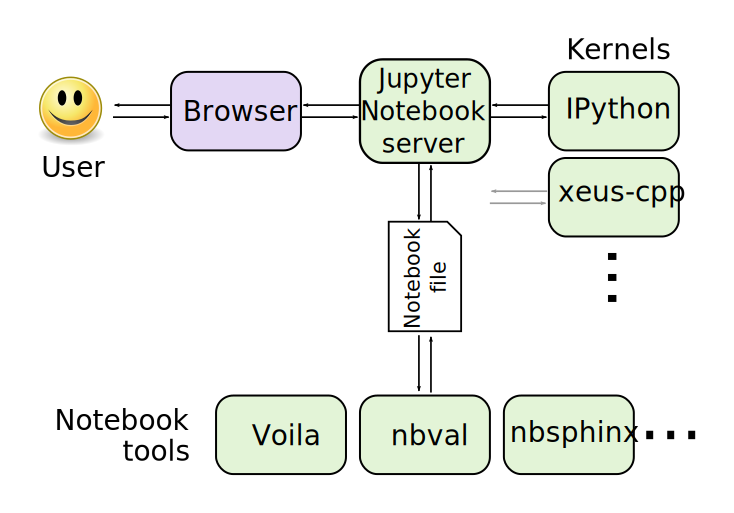
\includegraphics[width=0.6\textwidth]{images/notebook_components.png}
  \caption{The architecture of the Jupyter Notebook, kernels, and tools
        which operate on notebook files}
  \label{fig:notebook-architecture}
\end{figure}


\subsubsection{Methodology}\label{sec:methodology}


\textbf{Proposed improvements of core components of Jupyter (WP2)}

We plan to make technical changes to the Jupyter Notebook software to support
real-time collaboration (\taskref{core}{collaboration}),
so that two or more people in different places can work together
on the same notebook. This would significantly enhance the value of
notebooks for collaborative research.
We will also work on making Jupyter software accessible to as broad a
range of users as possible (\taskref{core}{accessibility}).

Further work to bring the code behind JupyterHub and Binder closer together
(\taskref{core}{jh-bh-conv}) will bring a range of benefits, allowing more
flexible sharing of notebooks along with access to remote computing resources
such as those available through EOSC.

Finally, we are explicitly allocating time in \WPref{core} for maintaining
Jupyter software, as well as new development (\taskref{core}{maintenance}).
Maintenance is crucial to creating reliable, sustainable software,
but its cost is often swept under the rug in funding applications
because of the perceived pressure to focus on novelty.

\textbf{Proposed improvements of the Jupyter ecosystem (WP3)}

We further propose improvements of the wider Jupyter ecosystem for
better scientific workflows. In particular, we have identified
possible improvements to:

\begin{itemize}
  \item Binder and its crucial software component \emph{repo2docker}
    (\taskref{ecosystem}{r2d-and-binder})

  \item Xeus, to better support the C++ programming language in notebooks
    (\taskref{ecosystem}{xeus-cpp})

  \item Interactive widgets, including tools for 3D visualisation to help
    people make sense of large amounts of data (\taskref{ecosystem}{jupyter-widgets})
\end{itemize}

\WPref{ecosystem} also includes work on tooling and guidelines for using
notebooks in education (\taskref{ecosystem}{teaching-tools}),
and for archiving computational environments to allow reproducible research
with a focus on the long term (\taskref{ecosystem}{reproducibility}).
We may create new open source software projects in these tasks,
but we will carefully review existing existing software, both in the
Jupyter ecosystem and beyond, to avoid unnecessary duplication of effort.

\textbf{Beyond the improvement of the Jupyter Project (WP4,
  WP5, WP6)}
Beyond the improvement to the software stack, we plan on
\begin{itemize}
\item Application, demonstration and evaluation of such novel services
  in multiple demonstrators, that cover research fields such as
  health, astrophysics, photon and neutron science, geosciences and
  mathematics, and also interests of participating SMEs (WP4)
\item Operating a \emph{European Binder Service} on the EOSC-Hub and
  enabling provision of Jupyter Services through the EOSC-Hub (WP5).
\item Producing \emph{training and education material} to disseminate
  the ability to do reproducible computational science using the tools
  we develop, among others. (WP6)
\end{itemize}

\medskip
\textbf{The science demonstrators}\label{sec:science-demonstrators-in-concept}


\medskip

\emph{Demonstrator: Astronomy (\taskref{applications}{astro})}\label{sec:concept-demonstrator-astronomy}

  The \href{http://cdsweb.u-strasbg.fr/}{Strasbourg Astronomical Data Center} (CDS) is scientific data
  center hosted by the Observatory of Strasbourg. The CDS plays a unique and
  essential role in astronomy by adding value to published and reference data.
  CDS runs astronomical services that
  provide data for the world-wide astronomy research community. Its three main
  services (SIMBAD, VizieR and Aladin) are heavily used with up to one million
  queries per day.  These services be accessed through web interfaces, mainly
  for human interaction, as well as through programmatic interfaces, including
  the standardized protocols defined by the International Virtual Observatory
  Alliance.

\begin{figure}[ht!]\centering
  \includegraphics[width=0.6\textwidth]{python-astro-citations}
  \caption{Mentions of programming languages in refereed Astronomy papers, extracted from ADS. Python usage has increased dramatically in the recent years.}\label{fig:python-astro-citations}
\end{figure}

  Python and notebooks are rapidly increasing in importance for astronomy
  research. Indeed, Python for Astronomy software ecosystem has known a
  constant steady growth in the latest years, as shown in
  figure~\ref{fig:python-astro-citations}. As Python and notebooks integrate
  well together, the Jupyter notebook as an analysis tool is becoming a hot
  topic in the astronomical world: large surveys like the LSST (Large Synoptic
  Survey Telescope) have endorsed the usage of the Jupyter platform for their
    data access portal \cite{lsst2017scienceplatform}.\\


  We will develop a Jupyter-based framework to efficiently access, explore,
  visualize and analyze reference data that are available through CDS services
  as a real example of using open astronomy data.
  We will provide scientific users with a set of customizable Jupyter notebooks
  for visualization and analysis tasks, providing a new level of
  interoperability with python libraries and notebooks as is highly demanded
  by the astronomy research community.

  The focus is on the two following user stories:
    \begin{compactitem}
        \item analysis of catalogue data results, up to billions of rows.
              Tabular data is the typical output of SIMBAD and VizieR data.
        \item modular dashboard-like interface providing a top level
              interactive view of the available data for a given astronomical
              object and enabling loading and analysis of those data.
    \end{compactitem}


\begin{figure}[ht!]\centering
  \includegraphics[width=1.0\textwidth]{astro-aladin-snapshot}
  \caption{Simbad objects, XMM and Hubble coverages overlaid on Digital Sky Survey imagery in the vicinity of the Horsehead nebula, and visualized in Aladin Desktop software.}\label{fig:astro-aladin-snapshot}
\end{figure}

  Access to the notebooks will be provided as a one-click action option from
  SIMBAD and VizieR results pages.
  Thus, providing with a one-click way of visualizing, filtering and analyzing
these potentially large tables will bridge the gap between access and analysis
of the data, with zero installation for the user.
  For specific science cases, we will explore rendering of notebooks with
  interactive widgets through "Voila", as to allow users not familiar with
  Python to benefit from the Jupyter notebook framework.
  Figure~\ref{fig:astro-aladin-snapshot} depicts typical data objects we want to analyse and interact with in the notebooks: images, catalogue data, datasets coverages.

  These new developments will be highly visible to the large number of astronomers who use the CDS services (50,000 unique visitors per month) and such tools are in high demand by these users.

  The CDS expertise in astronomy data and interfaces will be profitably combined with expertise of BOSSEE partners to ensure the deployment of high quality widgets (Simula, WildTree Tech, QuantStack).

\medskip
\textbf{Demonstrator: enriched teaching with Jupyter (\taskref{applications}{teaching})}\label{sec:concept-demonstrator-teaching}

  As argued in Task~\taskref{ecosystem}{teaching-tools}, the Jupyter
  ecosystem offers a versatile environment which has been widely
  adopted in higher education in the recent years. École
  Polytechnique, Université Paris-Sud and other participants from this
  project have been early adopters (see the description of \site{EP}
  and \site{UPSUD}).

  \begin{figure}[ht!]\centering
  \includegraphics[width=.45\textwidth]{images/teaching-cling}\quad
  \includegraphics[width=.45\textwidth]{images/teaching-graphs}
  \caption{Jupyter based teaching material from Paris Sud. On the
    left: an exercise sheet for the course \emph{introduction to
      programming}; this instructor version showcases interactive C++
    execution and automatic grading configuration menus. On the right:
    interactive slides for a graph theory course.
    course.}\label{fig:teaching-cling}
  \end{figure}

  We learned the hard way that deploying the Jupyter environment at a
  large scale (e.g. for a university) requires specialized expertise
  (DevOps, software development, ...) which impediments its adoption
  by the greatest number of people. High quality hosted solutions
  (e.g. cocalc, gryd) do exist but are not the final solution when it
  is desired to get higher control on private data, integration with
  the local infrastructure (authentication, shared drive, e-learning
  environment, dedicated hardware, ...), or to use local computing
  resources rather than paid services.

  Further improving the Jupyter environment for education, while
  leveraging it to the greatest number, are therefore key motivations
  for the following tasks of this proposal:
  \begin{itemize}
  \item Tasks~\taskref{core}{jh-bh-conv}
    and~\taskref{eosc}{jh-bh-deployment} will greatly ease the
    deployment of Jupyter environments, with tight integration in the
    existing local infrastructure and full customizability by the
    teachers.
  \item Task~\taskref{ecosystem}{teaching-tools} will improve the
    interoperability with existing e-learning systems, and further
    develop teaching aids for, e.g., material sharing,
    (self)-evaluation, and grade management.
  \item Task~\taskref{applications}{math} will support teaching
    in mathematics through better support for real-time interactivity.
  \item Task~\taskref{ecosystem}{xeus-cpp} will support teaching
    in computer-science and scientific programming through
    better C++ integration in the notebook and will allow to first classe students to focus on the
    syntax of the language without distractions such as compiling and
    linking a program.
  \item Task~\taskref{eosc}{eosc} will ease publication and FAIR
    access to course material.
  \end{itemize}

\medskip
\textbf{Demonstrator: Visualisation and control of fluid dynamics in
  Jupyter notebook (\taskref{applications}{application-gpu})}\label{sec:concept-demonstrator-gpu}


In recent years, the lattice Boltzmann method (LBM) emerged as an
interesting alternative to more established methods for fluid flow
simulations. Sailfish-cfd \cite{januszewski2014sailfish} is an open
source implementation of the LBM on General Purpose Graphical Processing
Unit (GPGPU) devices. It is written in Python with real-time
generation of CUDA-C code.  In order to harvest capabilities of GPGPUs
one needs to access the specialized hardware, which usually is
available to researchers as remote HPC resources.  The typical fluid
dynamics research workflow consists of three stages: preparing
boundary conditions, running a simulation, and data analysis. The
first and last stage require capable and responsive user interface for
maniputation and inspection of 3d data.  The Jupyter 3d visualisation
widgets developed in \taskref{ecosystem}{jupyter-widgets} can fulfil
such needs.

Based on previous experience with K3D-jupyter\cite{K3D}
widgets we know that web browser based software can display moderate
dataset during the simulation. As the dataset is becoming larger the
visualisation in the browser turns out to be nontrivial due to
limitations of the browser itself and required large data transfers. It is
an open question how much of data processing should be performed on
server-side and what can be done on the client hardware (i.e. in the
widget in the browser side of the user). Our
experience suggests that there is no clear answer and it depends on
the size of the data and its nature. For example, volume rendering
technique can be very effective on the browser side but infers large data
transfers. One can perform it the server-side, in a distributed way if
the simulation uses many nodes, but the interactivity is limited by
network latency. We will attempt to provide practical
solutions to this issue.
%

\medskip
\textbf{Demonstrator: Geosciences (\taskref{applications}{geoscience})}\label{sec:concept-demonstrators-geo}

The amount of geospatial data from a variety of sources, including satellite observations, 4D simulations and in-situ observations, contributed by volunteers
or state agencies keeps increasing. In many disciplines, managing this large volume
has become a challenge, and the old approach of downloading datasets for a local
analysis has become intractable.

The heterogeneity of the tools used in different institutions to deal with
large geographical datasets makes it difficult for researchers to share the outcome
of their work in a reproducible fashion.

In this context, Jupyter is now emerging as a standard exploration tool for
geospatial analysis, climate science, geology and by data providers in these areas.

To mention a few,
\begin{itemize}
\item
   the \emph{PanGeo} platform \cite{Pangeo2018} (Funded by the NSF, NASA, and the
   Alfred P. Sloan Foundation) is built upon Jupyter, JupyterHub, Binder, and Dask.
\item
   the \emph{Joint Research Centre Earth Observation Data and Processing Platform}
   (JEODPP) \cite{Soille2018} relies on Jupyter, JupyterHub and ipyleaflet as
   its main user interface.
\item
   the \emph{Google Earth Engine} platform also offers a jupyter-based user
   interface allowing the visual exploration of the data with ipyleaflet
   \cite{GEEJupyterLeaflet2017}.
\end{itemize}

In these three cases, deferred processing is used to restrict computation to
the extent of the area displayed in the map viewer, which allowed these
platforms to scale up to petabytes of data. In all examples, interactive
visualization is a key feature of the platform. Beyond tile-based
2-D visualization, the ability to efficiently process and visualize vector
or 3-D  data is also becoming critical.

The BOSSEE team, which comprises the main authors of the technologies upon
which these platforms are built (Jupyter, JupyterHub, Binder, ipyleaflet),
together with the Department of Geosciences of the University of Oslo, are
in a unique position to bring these technologies together in the context of
EOSC.

This demonstrator will focus on tools for two transversal research projects

\begin{itemize}
\item LATICE (Land-Atmosphere Interactions in Cold Environments)
\url{https://www.mn.uio.no/geo/english/research/groups/latice/}
\item EarthFlows (Interface Dynamics in Geophysical Flows)
\url{https://www.mn.uio.no/geo/english/research/groups/earthflows/}
\end{itemize}

The work items for this demonstrator fall in two main categories:
visualization and geographical data processing tools.

\textbf{Teaching geo-sciences with Jupyter}\TODO{Anne - please see my
  comments in email - this looks odd here (Hans)}

Beyond their use in scientific research, these development will be used in
the class room for teaching master's students with best practices in open
science.

\TODO{The transversal research plays into the desired ``services that
  encourate collaborative interdisciplinary work'' that are desired
  by this call; this is good. Can you imagine that some of these
  facilities can be used via the EOSC? That would be a good
  addition. For example, one could use the BinderHub installation
  that we expect on the EOSC. }

\medskip
\textbf{Demonstrator: Nuclear Medicine application (\taskref{applications}{opendose-analysis})}\label{sec:concept-demonstrators-opendose}

  % Scientific description
  Nuclear Medicine is a field of medicine where radioactive material
  (radiopharmaceutical) is used for diagnostic and therapy. Even though the
  majority of Nuclear Medicine procedures (90\% according to successive EANM
  surveys) are diagnostic examinations, therapeutic applications tend to
  develop and drag more and more attention, for example for the treatment of
  neuroendocrine tumours \cite{Bodei2009}.

  The formalism used to objectively characterise the irradiation process is
  similar for both application types: it was introduced in the late 60s by the
  MIRD (Medical Internal Radiation Dose) committee of the American Society of
  Nuclear Medicine (SNM). This formalism \cite{loevinger1991mird} requires two
  independent quantities; the radioisotope cumulated activity ($Bq.s$) in the
  source (tissue/organ) and the mean absorbed dose to a given target
  (tissue/organ) per radioisotope disintegration (S-value,
  $Gy.Bq^{-1}.s^{-1}$). The S-value calculation requires a clear definition of
  the geometry of the patient (or the model) and radioisotope decay
  characteristics, it can be expressed as a linear combination of
  yields/energies ($J$) and Specific Absorbed Fractions (SAF, $g^{-1}$).

  The calculation of SAFs involves radiation transport modelling and energy
  deposition scoring in anthropomorphic models, usually based on Monte Carlo
  simulation. Historically, SAFs were computed from mathematical models -
  simplistic approximations to human geometry. The advent of voxel-based
  computational models requires a new appraisal of dosimetric data. For
  example, the models recently proposed by the International Commission on
  Radiation Protection (ICRP) include 140 possible radiation sources, leading
  to around 20000 source/target combinations \cite{ICRP2009ICRPPhantoms}. The
  production of SAFs for these models for all possible source regions,
  radiation types and energiesimpul represent an important computation time
  (millions of CPU hours).

  The OpenDose project \cite{Chauvin2017} is a collaborative effort to generate
  reference dosimetric data using various Monte Carlo codes across different
  teams. The collaboration includes at the moment 14 research teams over 18
  institutes.  The idea is to trigger the collaborative development of a
  reference database, freely available, proposing dosimetric data applicable in
  a context of nuclear medicine dosimetry (for therapy and diagnostic
  applications). A major aspect of the project is the development of tools
  ensuring traceability and reproducibility of generated results.

  % Technical description
  OpenDose data is produced using the five most represented Monte Carlo
  simulation software in medical applications: Geant4/GATE, MCNP, EGS, PENELOPE
  and Fluka. Each simulation consists of calculating radiation transport in
  anthropomorphic models for specific parameters (source organ, particle type,
  energy, model and number of primaries to simulate). Every simulation produces
  binary (3D matrices) and ASCII files for a total of $\sim$150MB / simulation.
  The 3D matrices contain energy deposited per voxels, and ASCII files contain
  pre-processed data corresponding to energy deposited per regions such as
  organs and tissues. These raw outputs are later processed into dosimetric
  data such as Specific Absorbed Fractions (SAFs) and S-values.

  Producing data for one model (ex. adult female) requires $\sim$30,000
  simulations, with the workload shared between the different teams and
  software.

  The data produced by all the teams is currently centralised at the Cancer
  Research Center of Toulouse (CRCT), processed and fed into a local SQL
  database at CRCT.

  This collaborative effort raises some challenges:
  \begin{compactitem}
  \item Data production: a total of 750,000 hours of CPU time is needed per
    model.
  \item Volume of data: one model represents TB of raw data that can be
    heterogeneous from the different teams.
  \item Data analysis: raw data has to be processed into dosimetric data in a
    robust and reproducible way.
  \item Database: has to be efficient and handle all the data (raw and
    processed).
  \item Visualization: display and compare results from all teams.
  \end{compactitem}

Figure
  \ref{fig:opendose_framework} shows the overall framework of the project and
  how data will be managed.

  \begin{figure}[t!]
    \centering
    \includegraphics[width=1.0\textwidth]{images/opendose_framework.pdf}
    \caption{OpenDose project overall framework including the unified data
    analysis to be developed in this task.}
    \label{fig:opendose_framework}
  \end{figure}

  By building a set of tools to access and process data, this will ensure the
  production of traceable and reproducible dosimetric data for the OpenDose
  project members.

  Another major aspect of the OpenDose collaboration is to provide an open
  access to the generated dosimetric data. For that purpose a website is under
  development to allow data download and simple dosimetry calculations. For
  users who need more advanced calculations, a dedicated Jupyter workspace will
  provide a set of tools to easily access, process and display the OpenDose
  data.

\medskip
\textbf{Demonstrator: Interactive Mathematics with Jupyter Widgets (\taskref{applications}{math})}\label{sec:concept-demonstrator-math}

  \TODO{Ideas to reinforce the ties with EOSC services welcome!}

  Computations have played a long time and ever increasing role for
  research and teaching in (pure) mathematics, to explore, search and
  check for conjectures, or better understand algorithmic ideas. This
  led to the development of a whole ecosystem of mathematical
  software, many of which are open source. Given the huge variety of
  mathematical objects and workflows, the Read-Eval-Print-Loop (REPL)
  paradigm -- on which Jupyter is based -- is particularly suitable:
  the user interacts with the system by typing commands that use its
  library of mathematical features, often combined with personal code.
  In fact, the REPL and notebook paradigms of Jupyter as well as some
  of its interactive features were largely inspired by that of
  computer algebra systems such as Maple, Mathematica, or SageMath.

  One major action of the OpenDreamKit project was to foster the
  convergence between the Jupyter and math software ecosystems:
  nowadays Jupyter can be used as a uniform user interface for most
  major systems: e.g. GAP, OSCAR, Pari/GP, SageMath, Singular, and
  even for C++ libraries. This interface is being widely adopted: for
  example, Jupyter has become the standard user interface for
  SageMath, enabling to phase out its former bespoke notebook; by now,
  thousands of jupyter notebooks for SageMath are publicly shared
  (6000+ on GitHub alone).

  Thanks to this prior art, the mathematical community will
  immediately enjoy all the benefits brought by EOSC-based generic
  Jupyter services, including eased collaboration, sharing, archival,
  and reproducibility.

  The next step to maximize attractivity and impact in the
  mathematical community, and this is the aim of this task, is to go
  beyond the REPL paradigm, and \textbf{leverage the real time
    interactivity and flexibility brought by Jupyter widgets for
    Mathematical purposes}. Think making it easy for a teacher or
  researcher to build and disseminate via the EOSC a mini applications
  or dashboard enabling the graphical exploration of a whole range of
  mathematical inputs, with real-time visualization of the associated
  outputs.

  The unique challenge comes from the huge variety of mathematical
  objects that the user may want to visualize and interact with, and
  the variety of graphical representations. Co-design is central here,
  as building a bespoke interactive visualization entails a
  combination of technology skills (e.g. javascript development) and
  business knowledge (designing the interaction and visualization).
  The role of Research Software Engineers is to leverage the
  technology by encapsulating the technical difficulties into flexible
  and easy to use tool boxes from which mathematicians can build
  mini-applications tailored to their needs.

  Within OpenDreamKit, we conducted experiments to explore this
  venue~\cite{ODK_D4.16}. One specific focus was to enable not only
  \emph{interactive visualization}, but also \emph{interactive
    editing}: being able to graphically modify the mathematical object
  being visualized; this enable the interactive exploration of how the
  modifications affect its properties, or to use the editor as input
  widget for a larger applications or dashboards. The outcome of this
  task are the development of two prototypes in SageMath
  (\software{sage-combinat-widget}, a library of widgets for
  combinatorics, and \software{sage-explorer} a generic dashboard for
  interactive browsing and introspection of mathematical objects), and
  contributions to \software{Francy}, an Interactive Discrete Math
  Framework for \software{GAP} and \software{SageMath}.

\medskip
\textbf{Demonstrator: Reproducible photon science workflows at
  European XFEL (\taskref{applications}{reproducibility-xfel})}\label{sec:concept-demonstrator-photonscience}


  European XFEL is a research facility that provides X-ray Free
  Electron Laser (XFEL) light to image structures at the nanoscale. It
  is currently the world's most brilliant laser, created in a 3.4km
  long tunnel, and supporting user experiments since September
  2017. These imaging capabilities from European XFEL and similar
  services from synchrotron and neutron sources, underpin lots of
  fundamental and applied research, in domains ranging from fundamental
  physics and material science to biochemistry and drug design. Some
  example data is shown in figure \ref{fig:photon-science-example}.

  All of the data recorded at European XFEL will be made freely
  available after an embargo period of three years
  \cite{EuXFEL-datapolicy-2017}. This provides scientific transparency
  and is expected to enable better exploitation of the data, as more
  researchers than those conducting the experiments have access to the
  results. If the analysis steps are not carefully recorded, there is a risk
  that the necessary understanding of the data is lost by the time it
  is made public or subsequently, greatly reducing its scientific
  value.

  We are keen to complement this open data access to the actual data
  with open access to reproducible data analysis, to confirm
  conclusions drawn and to significantly lower the barriers for
  re-analysis with new tools or for new research purposes.

  A task in the EC funded project Photon and Neutron Open Science
  Cloud (PaNOSC) is using the Jupyter Ecosystem tools as they are in
  2019 to provide interactive data analysis services to complement the
  data: through use of Jupyter Notebook and exploitation of the
  mybinder.org service, this activity will reduce the barrier for
  interactively exploring the data, understanding and making use of
  the data, and to do this through a central portal such as EOSC.

  Here, we combine and use the new developments of this
  proposal to enable new qualities of open science services, and to
  demonstrate the potential impact of these improvements for a wide
  set of EOSC services through a demonstrator in Photon Science.

  \medskip

\begin{figure}[tb]
    \centering
    \includegraphics[height=0.27\textheight]{images/photon-science-prototype1.png}
    \includegraphics[height=0.27\textheight]{images/photon-science-prototype2.png}
    \caption{Prototypes for data analysis of 2d x-ray detector images
      in the Jupyter notebook, relating to the
      photon science use case.
      % task reference in caption doesn't work
      % \taskref{applications}{reproducibility-xfel}.
      \emph{(Left)} Data from crystallography
      scattering experiment. \emph{(Right)} Azimuthal integration of detector
      data as one step in the data analysis workflow.}
    \label{fig:photon-science-example}
  \end{figure}


  \textbf{Context}

  The very first experiments at European XFEL
  produced as little as 45 terabytes of data on average, but as the
  facility develops, the amount of data produced per time is expected
  to grow substantially: Given the rate of light pulses, there is the
  potential to produce up to a petabyte of data within the beam time
  of one experiment (typically one week). These significant amounts of
  data need to be complemented by complicated workflows to convert the
  data into insight through data analysis. Derived results of such
  data analysis are typically much smaller in size and useful to
  archive together with the raw data. To explain how they have been
  obtained, the particular workflow of data analysis also needs to be
  archived.

  \medskip
  \textbf{Vision}

  At European XFEL we will use Jupyter notebooks to facilitate
  this workflow: the simplest model would be to use one notebook per
  workflow. Once the data capture from the experiment is completed,
  this notebook can be executed (without being displayed in a web
  browser) to start processing the data. When the notebook has
  completed execution, it is saved, and contains the analysis results
  (it may of course also created files on disk as part of the
  process).

  A particularly useful aspect of the notebooks is that they mix data
  analysis commands with outputs, and that the notebook provides a
  complete (and thus reproducible) summary of the data analysis when
  it succeeds with the execution. Should the execution fail, for
  example half-way through the notebook, then derived results obtained
  prior to the error occurring are preserved and can be inspected. The
  error is embedded in the notebook and appears after the command that
  has triggered the error; which helps with debugging the process.

  This is of particular interest as the data analysis processes at
  European XFEL may fail not because of software errors but due to
  variation in the data that require (manual) expert adjustments of
  parameters. The ``failure'' of such an analysis workflow
  (represented through the Notebook) is thus not exceptional, but a
  common occurrence. The scientist conducting the experiment is
  sufficiently skilled to modify the parameters and wants to either
  re-execute the notebook from the beginning or to continue from the
  point of failure. The notebook caters for both use cases. The
  modified notebook would need to be preserved of course to provide
  reproducibility of the derived results that the notebook has
  computed.

  We are aiming for re-executability of the notebook for the lifetime
  of the data. The life time of the archived data at European XFEL is
  currently guaranteed for 5 years and aimed to be 10 years
  \cite{EuXFEL-datapolicy-2017}. It is possible though, that data used
  for publications will be preserved for longer, and it would be
  highly desirable to keep the data analysis re-executable for the
  same period of time, potentially well exceeding 10 years.


\draftpage
% ---------------------------------------------------------------------------
%  Section 1.4: Ambition
% ---------------------------------------------------------------------------
\TOWRITE{ALL}{Proofread 1.4 Ambition pass 2}

\subsection{Ambition}

\eucommentary{1-2 pages}

\eucommentary{-- Describe the advance your proposal would provide
  beyond the state-of-the-art, and the extent the proposed work is
  ambitious. Your answer could refer to the ground-breaking nature of
  the objectives, concepts
  involved, issues and problems to be addressed, and approaches and methods to be used.\\
  -- Describe the innovation potential which the proposal
  represents. Where relevant, refer to products and services already
  available, e.g. in existing e-Infrastructures.}

BOSSEE's ambition is to improve the global accessibility of scientific
tools, results, ideas, data and data analysis; enabling collaboration among researchers and between researchers and the public.

The world's computational resources are
constantly growing and science is producing ever-more useful and
interesting data.  But how do we enable the European and global
communities to make use of that data?  And not just researchers, but
the public as well?  Open science is a principle of making research
results as broadly accessible and useful as possible.  The first,
minimal step for this is making publications free to access.  The
second step for computational research is to make code and data
publicly accessible, enabling transparency and facilitating
reproducibility and verifiability of results.  But merely making these
resources technically available is not the best we can do.  There can
be many challenges with software, such as environment specifications
and resource requirements, that can be an impediment to the transition
from `technically available' to `practically useful.'  With the tools
of the open source open science community and the resources of the
European Open Science Cloud, we can do better.

The Jupyter ecosystem consists of a large, global community of
developers and researchers producing software focused on interactive
computation and communication, and is widely used by millions of
individuals in numerous scientific fields, ranging from molecular
biology \cite{Wang2016} to materials science \cite{Hughes2014},
astronomy \cite{Baron2017} and climate science
\cite{Laken2015,Laken2015b}.  Jupyter software is permissively
licensed under the Berkeley Software Distribution (BSD) license,
allowing anyone to use Jupyter software for free, and even build
derivative commercial products, as has been done in the cases of
Google Colaboratory, Microsoft Azure Notebooks, IBM Watson Studio, and
others \TOWRITE{cite}.  By contributing to the Jupyter ecosystem,
\TheProject maximises its impact, immediately benefiting the existing
large Jupyter community, and increasing the likelihood that
\TheProject's results will be maintained by the community after the
end of formal funding.

When it comes to Jupyter and Open Science, we aim to improve the
\textit{status quo} by bringing the two together:

\begin{itemize}
\item Improve software in the Jupyter ecosystem to better serve open
  science.
\item Enable researchers and the public to better perform and benefit
  from open science, through software, services, and education.
\end{itemize}

Open Science that truly benefits society must be more than merely
technically accessible.  Individuals must be able to find the
resources they want and interact with them.  Ideally, they should be
able to ask new questions of models and data published by those that
came before.  This is where \TheProject fits in.  Excellent research
is being performed in all scientific fields, but making those results
practically accessible and engaging to others is a challenge.
Jupyter notebooks enable publishing code and data in a form that is
interactive, where readers can see code, run it, and see results.
They can then modify the code and produce new data and charts that the
first authors may not have considered.  Jupyter does not solve the
software installation problem, however, which can be significant for
scientific software.  For a publication to be truly interactive or
reproducible, it must include a computational environment (or a
sufficiently precise description of one such that it can be recreated)
in order to reliably be able to run for another individual.  Services
and tools such as Binder and repo2docker facilitate this.  By
publishing a description of the requirements to run the software,
repo2docker is able to recreate a computational environment with
everything needed to run the software, including a Jupyter
environment for interactively exploring the resource.  Binder wraps
this in a web service, enabling immediate, free sharing of
computational results on the web, with no requirements of readers
other than a web browser.  By deploying Binder or similar services on
EOSC infrastructure, EOSC enables researchers to make their results
available to the public, and enables the public to interact with the
science they are funding.

By cooperating with specific applications from diverse domains in science and education,
we ensure and demonstrate that the work is valuable to a broad community of researchers, students, educators, and the public.

All together, Jupyter and Binder enable the migration of the open
science community from static publication to truly interactive,
reproducible publications.


%%% Local Variables:
%%% mode: latex
%%% TeX-master: "proposal"
%%% End:

%  LocalWords:  eucommentary textsuperscript textregistered textsuperscript specialised
%  LocalWords:  textregistered recomputation textbf textbf rigourous centred flagshsip
%  LocalWords:  subsubsection realisation textit


\draftpage
% ---------------------------------------------------------------------------
%  Section 2: Impact
% ---------------------------------------------------------------------------
% ---------------------------------------------------------------------------
%  Section 2: Impact
% ---------------------------------------------------------------------------


\section{Impact}
\label{sec:impact}
\TOWRITE{ALL}{Describe impact}

\begin{figure}[ht]\centering
  \includegraphics[width=0.9\textwidth]{use-cases-binder-logbook-solution.png}
  \caption{A typical use case for Jupyter notebooks in research.
            Image by Juliette Belin for the OpenDreamKit project, used under
            CC-BY-SA.}\label{fig:use-cases-binder}
\end{figure}


\subsection{Expected Impacts}

\eucommentary{Please be specific, and provide only information that applies
to the proposal and its objectives. Wherever possible, use quantified
indicators and targets.\\
Describe how your project will contribute to:\\
-- the expected impacts set out in the work programme, under the relevant topic
(including key performance indicators/metrics for monitoring results and impacts);\\
-- improving innovation capacity and the integration of new knowledge
(strengthening the competitiveness and growth of companies by developing
innovations meeting the needs of European and global markets; and, where
relevant, by delivering such innovations to the markets;\\
-- any other environmental and socially important impacts (if not already
covered above).\\
Describe any barriers/obstacles, and any framework conditions (such as
regulation and standards), that may determine whether and to what extent
the expected impacts will be achieved. (This should not include any risk
factors concerning implementation, as covered in section 3.2.)}

\begin{center}
\begin{tabular}{|m{.3\textwidth}|m{.7\textwidth}|}\hline
  Expected impact & \\\hline


  Integrating co-design into research and
  development of new services to better support scientific, industrial and
  societal applications benefiting from a strong user orientation &
  The Jupyter tools have always been driven by a close connection to users; since
  the project began as IPython in 2001, many of the developers have been
  scientific researchers using the tools as they developed them. More recently,
  when Jupyter has benefitted from dedicated developer time, developers have
  remained in academic institutions, in the kind of role now referred to as
  'research software engineers', allowing day-to-day interactions with
  researchers using Jupyter in a wide range of fields.

  By supporting developers in various research institutions where the improvements
  will be used as they are developed, \TheProject will continue this invaluable
  collaboration.
  \\\hline

  Supporting the objectives of Open Science by
  improving access to content and resources, and facilitating interdisciplinary
  collaborations &
  We expect the use of notebooks in EOSC to improve access to scientific code,
  and the data which it handles. By combining code and explanation in a convenient
  digital document, notebooks encourage publishing workflows, whereas code in
  scripts or manual interactive workflows are often kept by the researchers who
  performed them. The focus on clarity and reproducibility also helps to ensure
  that data is meaningfully accessible, by preserving essential understanding to
  make sense of the raw data.

  We have already seen a good example of the Jupyter ecosystem facilitating an
  interdisciplinary collaboration: the LIGO scientific collaboration shared
  notebooks detailing the data processing steps which led to the discovery of
  gravitational waves, using the Binder service to allow anyone to re-compute
  the published plots. Scientists with no background in gravitational waves
  studied these notebooks and improved the signal processing.
  In this proposal, we want to provide this ability to a wider audience through
  EOSC, including for disciplines which rely on processing much larger volumes of
  data. \TOWRITE{ALL}{Citation for the LIGO story?}
  \\\hline

  Fostering the innovation potential by opening up
  the EOSC ecosystem of e-infrastructure service providers to new innovative
  actors &
  Jupyter is a collection of open source software built around openly documented
  protocols and formats, along with familiar technologies such as HTML and the
  Python programming language. It's easy for third parties to create new
  tools and services using and integrating Jupyter, as evidenced by the thriving
  ecosystem of tools already in development, both by commercial and non-commercial
  actors. To highlight just one example, the first version of the popular Binder
  service was developed by a group at the Howard Hughes Medical Institute,
  working independently of the core Jupyter maintainers, but building on the
  powerful capabilities provided by Jupyter.
  \\\hline

\end{tabular}
\end{center}



\clearpage

% ---------------------------------------------------------------------------
%  Section 3: Implementation
% ---------------------------------------------------------------------------

\section{Implementation}
\COMMENT{Typical granularity: 5-8 work packages with 3-5 tasks and one
  deliverable per task; 10 milestones}

\subsection{Work Plan --- Work packages, deliverables and milestones}
\label{sect:workplan}

\eucommentary{Please provide the following:\\
\begin{compactitem}
\item
brief presentation of the overall structure of the work plan;
\item
timing of the different work packages and their components (Gantt chart or similar);
\item
detailed work description, i.e.:
\begin{compactitem}
\item
a description of each work package (table 3.1a);
\item
a list of work packages (table 3.1b);
\item
a list of major deliverables (table 3.1c);
\end{compactitem}
\item
graphical presentation of the components showing how they inter-relate (Pert chart or similar).
\end{compactitem}
}

\subsubsection{Overall Structure of the Work Plan}\label{sec:workplan-structure}
\ifgrantagreement
The
\else
As shown in Figure~\ref{fig:wplist}, the
\fi

work plan is broken down into
six work packages:
\WPref{core} about maintaining the core Jupyter software infrastructure,
\WPref{ecosystem} for developing the ecosystem of software surrounding Jupyter,
\WPref{applications} for building applications to demonstrate the efficacy and guide the development
of core infrastructure,
\WPref{eosc} for operating services built on these
components and collaborating with existing EOSC stakeholders,
\WPref{education} for educating the public on Open Science best practices with the project's tools
and fostering diversity in the research and software communities.
This is complemented by
the usual management  work package
(\WPref{management}). The Gantt chart on
Page~\pageref{fig:gantt} illustrates the timeline for the various
tasks for these work packages.
%, including inter-task dependencies.

\ifgrantagreement\else
%\makeatletter\wp@total@RM{management}\makeatother
\wpfigstyle{\footnotesize\def\tabcolsep{3.5pt}}
%\wpfig[pages,type,start,end]
{\wpfig}
\fi

\subsubsection{How the Work Packages will Achieve the Project Objectives}
\label{sssec:how_the_work_packages_will_achieve}

% (Section~\ref{sect:objectives},page~\pageref{sect:objectives})
...


\gantttaskchart[draft,xscale=.33,yscale=.33,milestones]

\ifgrantagreement\else
\newpage
\subsubsection{Deliverables}\label{sec:deliverables}
\inputdelivs{9.3cm}
\fi

\newpage
\subsubsection{Milestones}\label{sec:milestones}
\eucommentary{Milestones means control points in the project that help to chart progress. Milestones may
correspond to the completion of a key deliverable, allowing the next phase of the work to begin.
They may also be needed at intermediary points so that, if problems have arisen, corrective
measures can be taken. A milestone may be a critical decision point in the project where, for
example, the consortium must decide which of several technologies to adopt for further
development.}



\paragraph{General Milestones}

\begin{milestones}
  \milestone[
    id=startup,
    month=12,
    verif={
      Completed all corresponding deliverables
      and preparation for deployment of prototype services is underway
      }
    ]
  {Startup, requirements, and prototype generic Jupyter service}
  {
  By milestone 1, we will have established the infrastructure
  for the project and begun prototyping development and deployment of services,
  engaging with the existing communities,
  coordinating plans for \TheProject with those of the wider Jupyter and open science communities,
  and prototyping operation of a generic Jupyter service
  for Open Science.
  EGI Infrastructure-as-a-Service (IaaS) cloud resources are available with a
  Service Level Agreement (SLA) for \TheProject.
  }

  \milestone[
    id=prototype,
    month=24,
    verif={
      Completed all corresponding deliverables and early users are able to access and test prototype services
    }
    ]
  {Generic Jupyter service and early local demonstrators}
  {
  By milestone 2, we will have deployed a generic Jupyter service for Open Science, and begun to experiment with early-adopter
  users and local demonstrators to guide further development of \TheProject,
  ensuring that development serves the needs of the community.
  An initial \TheProject Service Management System shall be available,
  and \TheProject services are integrated with the EOSC Marketplace,
  and AAI Cloud services.
  }

  \milestone[
    id=community,
    month=36,
    verif={Completed all corresponding deliverables and services
    are operational and ready for public testing}
    ]
  {Demonstrator services and community engagement}
  {
  By milestone 3, demonstrator services should be useful and accessible
  to a broad range of users.
  By this point, we will have training materials and run
  workshops to train users in Open Science,
  making use of operational \TheProject services,
  gathering feedback to guide the further development of \TheProject.
  \TheProject Service Management System is fully compliant with the EOSC Service Management practices.
  }

  \milestone[
    id=final,
    month=48,
    verif={Completed all corresponding deliverables and reported progress at the final project review}
  ]
  {Full EOSC integration, adoption, sustainability, and evaluation}
  {
  By this point, all \TheProject services should be operational, available via EOSC-hub,
  and the generic Jupyter service TRL 8.
  Through community engagement via workshops, conferences, and other media,
  the services should have established groups of users,
  benefiting from these services and improving the Open Science landscape
  on EOSC and beyond.
  At the end of the project,
  we will have engaged with the community to evaluate
  the prototype EOSC services,
  identified which services and tools shall be sustained beyond the life of the project,
  and developed a sustainability plan for
  how this may be achieved under community support and leadership.
  }

\end{milestones}


% ---------------------------------------------------------------------------
% Include Work package descriptions
% ---------------------------------------------------------------------------

\newpage
\subsubsection{Work Package Descriptions}\label{sec:workpackages}
%%% work package style may be broken -- fix this!!

\ifgrantagreement
\begingroup
% Note: in the grant agreement, The workpackage description must not appear.
% Yet we want to compile them to get all the metadata right
% Current hack: compile them anyway, reset the page number
% appropriately, and remove them a posteriori with pdftk. We set the
% color to red to make it more visible in case we forget to remove
% them.
% See grantagreement rule in the Makefile
\newcounter{savepage}
\setcounter{savepage}{\value{page}}
\color{red} % To make sure we indeed remove the pages
\fi

\enlargethispage{1cm}

%% Local WP number counter - should possibly be global and hidden?
\begin{workplan}
\TOWRITE{ALL}{Proofread WP 1 Management pass 1}
\begin{draft}
\TOWRITE{PS (Work Package Lead)}{For WP leaders, please check the following (remove items
once completed)}
\begin{verbatim}
- [ ] have all the tasks in this Work Package a lead institution?
- [ ] have all deliverables in the WP a lead institution?
- [ ] do all tasks list all sites involved in them?
- [ ] does the table of sites and their PM efforts match lists of sites for each task?
      (each site from the table is listed in all relevant tasks, and no site is listed
      only in the table or only at some task)
\end{verbatim}
\end{draft}

\begin{workpackage}[id=management,type=MGT,wphases=0-48!.2,
  title=Project Management,
  short=Management,
  lead=SRL,
  CDSRM=3,
  EGIRM=3,
  EPRM=3,
  INSERMRM=3,
  QSRM=3,
  SILRM=3,
  SRLRM=24,
  UIORM=3,
  UPSUDRM=3,
  WTTRM=3,
  XFELRM=3,
  swsites
]
\begin{wpobjectives}
The main objective of WP1 is to establish and maintain an effective contract, project, and operational management approach ensuring:

 \begin{compactitem}
    \item Timely and successful implementation of the project; including administrative and legal coordination
    \item Technical management and quality assurance
    \item Risk and innovation management of the project as a whole; including data and IPR management
    \item Smooth communication and interaction with the EC and other interested parties

 \end{compactitem}
\end{wpobjectives}

\begin{wpdescription}
The project will be managed by Simula, which has extensive experience in administering and leading EU funded and national projects. The coordinator together with the WP leaders, will be responsible for monitoring WP status, coordination of work plan updates and annual internal progress reports. The project management structure and roles of partners in the consortium are presented in \ref{sect:mgt}.

\end{wpdescription}

\begin{tasklist}

\begin{task}[
  title=Administrative Management,
  id=admin,
  lead=SRL,
  PM=24,
  wphases={0-48},
  partners={CDS,EGI,EP,INSERM,QS,UIO,UPSUD,SIL,WTT,XFEL}
]
The task includes the following activities:
\begin{compactenum}
\item Preparation, distribution and maintenance of all contractual documents (Consortium Agreement, Grant Agreement and all other legal frameworks)
\item Establishment of appropriate communication and collaborative environment for the consortium, as well as the EC and other relevant academic and industry stakeholders (the project website, intranet and communication procedures) to organise transfer of knowledge, present and promote project results (\localdelivref{infrastructure});
\item Organisation of project review and progress meetings;
\item Performing qualitative and quantitative risk analysis, planning risk mitigation and control
\item Progress and Financial Reporting to the EC;
\item Data and IPR Management will be managed in accordance with agreed rules stated in the Consortium Agreement and in accordance with the Data Management Plans (\localdelivref{data-management-plan}, \localdelivref{innovation-management-plan}).
\end{compactenum}
\end{task}

\begin{task}[
  title=Technical Project Management,
  id=project-management,
  lead=SRL,
  PM=24,
  wphases={0-48},
  partners={CDS,EGI,EP,INSERM,QS,UIO,UPSUD,SIL,WTT,XFEL}
]
The project scientific and technical management ensures coherent quality and soundness of the work and results. A quality assurance plan will be developed by \site{SRL}, involving all partners, and will be followed up regularly. It will address the reviews and approval of technical reports and deliverables. In addition, the Project Coordinator with the help of the coordination team will regularly review technological risks and recommend mitigation plans to minimise or remove them. This will be reported on at each Reporting Period in the project's Technical Report.
\end{task}

\begin{task}[
  title=Innovation Management,
  id=innovation-management,
  lead=SRL,
  PM=6,
  wphases={0-48},
  partners={CDS,EGI,EP,INSERM,QS,UIO,UPSUD,SIL,WTT,XFEL}
]
One of the most important criteria for success for the BOSSEE project is to bring the project results into use. Therefore, exploitation routes will be sought whenever possible. In order to create a common understanding within the Consortium of how we can best shepherd an idea all the way from conception to realisation and exploitation, the Coordinator will be responsible for the preparation and realisation of an Innovation Plan. This plan will assure that research activities meet the required milestones and produce outputs fully aligned with the project objectives. All research activities will go through an initial process where the exploitation opportunity is identified along with the main stakeholders for the exploitation opportunity and an IP owner
(\localdelivref{innovation-management-plan}).
\end{task}

\end{tasklist}


\begin{wpdelivs}

% Rationale:
% - Eugenia recommended to have two deliverables about Data Management Plan, one early, and one at the complete end.
% - Having the Data Management Plan draft and Innovation plan at M9
%   gives some material in case we have an informal review at M9. Also
%   those are easy ones with no dependencies on progress; just
%   something to take care of at some point over the course of a few
%   weeks. So this spreads the load.

\begin{wpdeliv}[due=1,miles=startup,id=infrastructure,dissem=PU,nature=DEC,lead=SRL]
  {Basic project infrastructure (websites, wikis, issue trackers, mailing lists, repositories)}
\end{wpdeliv}

\begin{wpdeliv}[due=9,miles=startup,id=data-management-plan-draft,dissem=PU,nature=R,lead=SRL]
  {Data Management Plan draft}
\end{wpdeliv}

\begin{wpdeliv}[due=9,miles=startup,id=innovation-management-plan,dissem=CO,nature=R,lead=SRL]
  {Innovation Management Plan}
\end{wpdeliv}

\begin{wpdeliv}[due=48,miles=final,id=data-management-plan,dissem=PU,nature=R,lead=SRL]
  {Data Management Plan}
\end{wpdeliv}

\end{wpdelivs}
\end{workpackage}
%%% Local Variables:
%%% mode: latex
%%% TeX-master: "../proposal"
%%% End:

%  LocalWords:  workpackage wphases wpobjectives wpdescription pageref wpdelivs wpdeliv
%  LocalWords:  dissem mailinglists swrepository final-mgt-rep compactitem swsites ipr
%  LocalWords:  TOWRITE tasklist delivref

\newpage
\TOWRITE{ALL}{Proofread WP 1 Management pass 1}
\begin{draft}
\TOWRITE{PS (Work Package Lead)}{For WP leaders, please check the following (remove items
once completed)}
\begin{verbatim}
- [ ] have all the tasks in this Work Package a lead institution?
- [ ] have all deliverables in the WP a lead institution?
- [ ] do all tasks list all sites involved in them?
- [ ] does the table of sites and their PM efforts match lists of sites for each task?
      (each site from the table is listed in all relevant tasks, and no site is listed
      only in the table or only at some task)
\end{verbatim}
\end{draft}

\begin{workpackage}[id=core,wphases=0-48,swsites,
  title=Structural improvements to Jupyter,
  short=Core,
  lead=SRL,
  SRLRM=16,
  UPSUDRM=4,
  XFELRM=4,
]
\begin{wpobjectives}
  \begin{compactitem}
    \item to support and maintain core Jupyter infrastructure in order to keep it healthy
         and useful for open science
    \item to develop new features in the core of Jupyter to bring it to a wider community
    \item to develop new features in the core of Jupyter to make it more effective
         in facilitating open science

 \end{compactitem}
\end{wpobjectives}

\begin{wpdescription}

Community-led open source software is critical to a sustainable future for open science.
Commonly used tools make up a shared infrastructure,
where investment in core components benefits the widest user community.
\TheProject is centered around the Jupyter project,
which is a collection of projects for interactive computing and
communicating computational ideas.

This work package is focused on developing and maintaining
the core of Jupyter.
In particular, we will help maintain these projects to meet the needs of the
Jupyter community, with a focus on needs for open science.
In addition, we will develop new features in the core of Jupyter
to bring it to a wider audience,
and to improve its usefulness to those working toward open science practices,
including via collaboration features
and accessibility.


\end{wpdescription}

\begin{tasklist}

\input{tasks/jupyterhub}

% \input{tasks/<name>}

\end{tasklist}


\begin{wpdelivs}
\begin{wpdeliv}[due=1,miles=startup,id=infrastructure,dissem=PU,nature=DEC,lead=SRL]
  {Some Deliverable}
\end{wpdeliv}

\end{wpdelivs}
\end{workpackage}
%%% Local Variables:
%%% mode: latex
%%% TeX-master: "../proposal"
%%% End:

%  LocalWords:  workpackage wphases wpobjectives wpdescription pageref wpdelivs wpdeliv
%  LocalWords:  dissem mailinglists swrepository final-mgt-rep compactitem swsites ipr
%  LocalWords:  TOWRITE tasklist delivref

\newpage
\TOWRITE{ALL}{Proofread WP 1 Management pass 1}
\begin{draft}
\TOWRITE{PS (Work Package Lead)}{For WP leaders, please check the following (remove items
once completed)}
\begin{verbatim}
- [ ] have all the tasks in this Work Package a lead institution?
- [ ] have all deliverables in the WP a lead institution?
- [ ] do all tasks list all sites involved in them?
- [ ] does the table of sites and their PM efforts match lists of sites for each task?
      (each site from the table is listed in all relevant tasks, and no site is listed
      only in the table or only at some task)
\end{verbatim}
\end{draft}

\begin{workpackage}[id=ecosystem,type=MGT,wphases=0-48!.2,swsites,
  title=Developing the Jupyter Ecosystem,short=Ecosystem,
  lead=SR,
  SR=16,
  UPSUD=4,
  XFEL=4,
]
\begin{wpobjectives}
 \begin{compactitem}
   \item objective...
 \end{compactitem}
\end{wpobjectives}

\begin{wpdescription}

Description of the work package
\end{wpdescription}

\begin{tasklist}
\begin{task}[title=Task title,
  id=task-id,lead=PS,PM=1,wphases={0-48!.2},
  partners={Simula,PS,XFEL}]
  The task includes the following activities
  \begin{compactitem}
  \item ...
    (\delivref{workpackage}{deliv-id})
  \end{compactitem}
\end{task}
\end{tasklist}


\begin{wpdelivs}
\begin{wpdeliv}[due=1,miles=startup,id=infrastructure,dissem=PU,nature=DEC,lead=SR]
  {Some Deliverable}
\end{wpdeliv}

\end{wpdelivs}
\end{workpackage}
%%% Local Variables:
%%% mode: latex
%%% TeX-master: "../proposal"
%%% End:

%  LocalWords:  workpackage wphases wpobjectives wpdescription pageref wpdelivs wpdeliv
%  LocalWords:  dissem mailinglists swrepository final-mgt-rep compactitem swsites ipr
%  LocalWords:  TOWRITE tasklist delivref

\newpage
\TOWRITE{ALL}{Proofread WP 1 Management pass 1}
\begin{draft}
\TOWRITE{PS (Work Package Lead)}{For WP leaders, please check the following (remove items
once completed)}
\begin{verbatim}
- [ ] have all the tasks in this Work Package a lead institution?
- [ ] have all deliverables in the WP a lead institution?
- [ ] do all tasks list all sites involved in them?
- [ ] does the table of sites and their PM efforts match lists of sites for each task?
      (each site from the table is listed in all relevant tasks, and no site is listed
      only in the table or only at some task)
\end{verbatim}
\end{draft}

\begin{workpackage}[id=applications,wphases=0-48,swsites,
  title=Science demonstrators,
  short=Demonstrators,
  lead=XFEL,
  EGIRM=7,
  CDSRM=12,
  INSERMRM=24,
  QSRM=6,
  SILRM=12,
  SRLRM=9,
  UIORM=12,
  UPSUDRM=20,
  WTTRM=3,
  XFELRM=36,
  EPRM=3,
]
\begin{wpobjectives}
  The objectives of this work package are
 \begin{compactitem}
   \item to guide the development of core tools by simultaneously
     developing and using applications in diverse fields with active
     scientists from these fields, and
   \item to demonstrate that the tools we develop are valuable to diverse
     fields of science, thus ensuring we develop e-infrastructure and
     services which can cater for a broad customer base of EOSC.
   \end{compactitem}
\end{wpobjectives}

\begin{wpdescription}

  Whilst the components issued from work packages  \WPref{core} and \WPref{ecosystem} will be
  made available as generic building blocks for EOSC services, this
  work package aims at building and deploying bespoke EOSC services
  targeting real-world cases.

  We have selected a number of applications in a variety of domains
  to demonstrate the broad impact of \TheProject, in particular in the
  areas of astronomy
  (\localtaskref{astro}), education
  (\localtaskref{teaching}), fluid dynamics
  (\localtaskref{application-gpu}), geosciences
  (\localtaskref{geoscience}), health
  (\localtaskref{opendose-analysis}), mathematics
  (\localtaskref{math}) and photon science and imaging
  (\localtaskref{reproducibility-xfel}).
  The context and vision for each of the demonstrators is described in
  section \ref{sec:science-demonstrators-in-concept} on page
  \pageref{sec:science-demonstrators-in-concept}.

  Working closely with the core developers of the Jupyter ecosystem will make it possible to
  go way beyond what is normally available "out-of-the-box" and to offer better solutions,
  thereby guiding further development of the core features.

  \medskip
  Our demonstrators will typically undergo two-stages: (i)
  development and testing of the services locally at the developing partner
  site. (ii) Making the service available through the European Open
  Science Cloud (EOSC).

  All demonstrators will deliver base-line services by making the
  relevant notebooks executable in the \emph{European Binder Service} instance that this
  project will deployed on EOSC. This will demonstrate
  the Jupyter service capabilities such as reproducibility, interactive
  widget use and visualisation, and show how these can
  enable new open science on EOSC.

  The particular workflows, data infrastructures and data policies for
  FAIR\footnote{Findable, Accessible, Interoperable and Reusable} sharing of data vary from one community and use-case to
  the other, or may not be fully defined yet. Therefore, this proposal
  does not enforce a specific way of handling data. Instead we
  will explore in the demonstrator tasks how existing data policies,
  infrastructure and workflows can be respected and integrated with
  authentication and authorisation, data management, and
  JupyterHub/Binder services on EOSC. EGI is a partner
  for all the tasks in this work package and will work with us to find the
  best integration solutions in the evolving EOSC
  infrastructure.

  In the EOSC-hub project EGI operates a Jupyter Hub service which is deployed 
  in a scalable mode on EGI IaaS Cloud. This Jupyter Hub is already integrated 
  with the EUDAT B2DROP and OneData data management services of EOSC, and will 
  be integrated, in the next 12 months, with the EUDAT B2SHARE service.
  The integrations enable users to move data between Jupyter notebooks and storage 
  sites of the EGI Federation (with Onedata), between Jupyter and storage sites 
  of the EUDAT federation (B2SHARE), and between Jupyter and their personal cloud 
  storage hosted in EUDAT (B2DROP). The WP4 use cases will evaluate these data management 
  integrations and EGI will bring the respective technology from EOSC-hub into the 
  services operated by \TheProject.

  For some of the demonstrators, authentication and authorization and/or
  data management are being addressed outside \TheProject.
  This is for instance the case for the photon science and astronomy
  demonstrators via \href{https://panosc-eu.github.io/}{PaNOSC} and
  \href{https://www.eso.org/public/announcements/ann18084/}{ESCAPE} projects, respectively.

\end{wpdescription}

\begin{tasklist}
% add tasks from task directory here
% \input{tasks/template}
\input{tasks/codesign-support}
\input{tasks/application-astro}
\input{tasks/teaching}
\input{tasks/application-gpu}
\input{tasks/application-geo}
\input{tasks/opendose-analysis}
\input{tasks/application-math}
\input{tasks/reproducibility-xfel}
\end{tasklist}



\begin{wpdelivs}
%\TODO{update due date and startup!}
%\TODO{update milestone!}

  \begin{wpdeliv}[due=12,miles=startup,id=codesign-support,dissem=PU,nature=R,lead=SRL]
    {Initial requirements for the demonstrators.}
  \end{wpdeliv}

  \begin{wpdeliv}[due=24,miles=prototype,id=local-services,dissem=PU,nature=R,lead=EP]
    {Report on the developments of the demonstrator services deployed locally.}
  \end{wpdeliv}

  \begin{wpdeliv}[due=36,miles=community,id=demonstrators,dissem=PU,nature=DEM,lead=EGI]
    {Demonstrators based on locally developed services made accessible
      through EOSC. Demonstrators may be developed further subsequently.}
  \end{wpdeliv}

  \begin{wpdeliv}[due=48,miles=final,id=applications-report,dissem=PU,nature=R,lead=XFEL]
    {Evaluation of demonstrators and case studies. Report on
      feasibility and user to guide EOSC service design.}
  \end{wpdeliv}

\end{wpdelivs}
\end{workpackage}
%%% Local Variables:
%%% mode: latex
%%% TeX-master: "../proposal"
%%% End:

%  LocalWords:  workpackage wphases wpobjectives wpdescription pageref wpdelivs wpdeliv
%  LocalWords:  dissem mailinglists swrepository final-mgt-rep compactitem swsites ipr
%  LocalWords:  TOWRITE tasklist delivref

\newpage
\TOWRITE{ALL}{Proofread WP 1 Management pass 1}
\begin{draft}
\TOWRITE{PS (Work Package Lead)}{For WP leaders, please check the following (remove items
once completed)}
\begin{verbatim}
- [ ] have all the tasks in this Work Package a lead institution?
- [ ] have all deliverables in the WP a lead institution?
- [ ] do all tasks list all sites involved in them?
- [ ] does the table of sites and their PM efforts match lists of sites for each task?
      (each site from the table is listed in all relevant tasks, and no site is listed
      only in the table or only at some task)
\end{verbatim}
\end{draft}

\begin{workpackage}[id=eosc,wphases=0-48,swsites,
  title=Services and EOSC Integration,
  short=EOSC,
  lead=WTT,
  EGIRM=12,
  EPRM=6,
  % INSERMRM=4,
  % QSRM=6,
  % SILRM=4,
  SRLRM=18,
  % UIORM=12,
  UPSUDRM=0,
  WTTRM=13,
  XFELRM=6,
  EPRM=10,
]
\begin{wpobjectives}
 \begin{compactitem}
   \item to support and develop BinderHub infrastructure based in the EU for
     science and education applications
   \item to scale this service by migrating to EOSC
 \end{compactitem}
\end{wpobjectives}

\begin{wpdescription}

This work package is focussed on developing and operating a publicly accessible
BinderHub service based in the EU.

The team of Project Binder provide a service at https://mybinder.org
which is public infrastructure powered by the software they develop.
mybinder.org is used to launch around 80000 "binders" every week and is
being used by researchers and teachers to make their work reproducible.

Although mybinder.org is very popular, there are currently only two
additional public BinderHubs worldwide. This means that there is a limited
expertise in operating and maintaining such public infrastructure.

In particular, we will help maintain the tools and documentation required
to operate public infrastructure like Binder to meet the needs of the
open-science community in the EU. In addition we will develop new features
for the BinderHub project that will bring it to a wider audience and improve
its usefulness for scientists based in the EU.

\end{wpdescription}

\begin{tasklist}
% add tasks from task directory here
% \input{tasks/template}
\input{tasks/eu-binder}
\input{tasks/eosc}
\input{tasks/deployment}
\end{tasklist}

\begin{wpdelivs}
    \begin{wpdeliv}[due=6,miles=community,id=eosc-annual-report,dissem=PU,nature=R,lead=EGI]
    {A report describing the technical and service provisioning integration activities required to ensure the provisioning of BOSSEE services through EOSC}
  \end{wpdeliv}
    \begin{wpdeliv}[due=18,miles=prototype,id=eosc-annual-report-1,dissem=PU,nature=R,lead=EGI]
    {First report on the technical and service provisioning integration activities and their status}
  \end{wpdeliv}
  \begin{wpdeliv}[due=18,miles=startup,id=openstack-openshift-documentation,dissem=PU,nature=R,lead=EP]
    {Documentation of how to deploy easily JupyterHub and BinderHub on OpenStack and OpenShift}
  \end{wpdeliv}
  \begin{wpdeliv}[due=24,miles=prototype,id=eu-binder-instance,dissem=PU,nature=R,lead=SRL]
    {Documentation and tools of how to easily deploy a public BinderHub on EU
    cloud infrastructure}
  \end{wpdeliv}
  \begin{wpdeliv}[due=36,miles=community,id=eosc-annual-report-2,dissem=PU,nature=R,lead=EGI]
    {Second report on the technical and service provisioning integration activities and their status}
  \end{wpdeliv}
  \begin{wpdeliv}[due=48,miles=final,id=binder-federation,dissem=PU,nature=R,lead=SRL]
    {Documentation on best-practices of operating a federation of BinderHubs}
  \end{wpdeliv}
  \begin{wpdeliv}[due=48,miles=final,id=eosc-annual-report-2,dissem=PU,nature=R,lead=EGI]
    {Final report on the technical and service provisioning integration activities and their status}
  \end{wpdeliv}
\end{wpdelivs}
\end{workpackage}
%%% Local Variables:
%%% mode: latex
%%% TeX-master: "../proposal"
%%% End:

%  LocalWords:  workpackage wphases wpobjectives wpdescription pageref wpdelivs wpdeliv
%  LocalWords:  dissem mailinglists swrepository final-mgt-rep compactitem swsites ipr
%  LocalWords:  TOWRITE tasklist delivref

\newpage
\TOWRITE{ALL}{Proofread WP 1 Management pass 1}
\begin{draft}
\TOWRITE{PS (Work Package Lead)}{For WP leaders, please check the following (remove items
once completed)}
\begin{verbatim}
- [ ] have all the tasks in this Work Package a lead institution?
- [ ] have all deliverables in the WP a lead institution?
- [ ] do all tasks list all sites involved in them?
- [ ] does the table of sites and their PM efforts match lists of sites for each task?
      (each site from the table is listed in all relevant tasks, and no site is listed
      only in the table or only at some task)
\end{verbatim}
\end{draft}

\begin{workpackage}[id=education,wphases=0-48,swsites,
  title=Education and Dissemination,
  short=Education,
  lead=INSERM,
  CDSRM=3,
  % EGIRM=4,
  % EPRM=0,
  INSERMRM=12,
  QSRM=4,
  SILRM=4,
  SRLRM=12,
  UIORM=12,
  UPSUDRM=12,
  WTTRM=4,
  XFELRM=8,
]
\begin{wpobjectives}
 \begin{compactitem}
   \item Train researchers in best practices for open and reproducible science
   \item Educate the community on the value of open science
 \end{compactitem}
\end{wpobjectives}


% Potential sources of inspiration: ODK's WP2 work package about dissemination:
% PDF: p.36 of https://github.com/OpenDreamKit/OpenDreamKit/raw/master/Proposal/proposal-www.pdf
% Sources: https://github.com/OpenDreamKit/OpenDreamKit/blob/master/Proposal/WorkPackages/DisseminationCommunityBuilding.tex

\begin{wpdescription}

Open science is entirely dependent on researchers adopting open practices.
In \TheProject, we are developing tools to facilitate these practices,
but they only work if researchers actually adopt them.
To this end, we will develop materials and run workshops,
training researchers.
Open science is not just of value to researchers, however.
One of the largest benefits of open science is that it makes science accessible to the broader public
who may not be members of the research community.
In addition to training researchers,
we will also train the public in how to make use of the open science research and services facilitated by \TheProject.

\end{wpdescription}

\begin{tasklist}
% add tasks from task directory here
\input{tasks/training}
\input{tasks/online-resources}
\input{tasks/website-general}
\end{tasklist}




\begin{wpdelivs}
\begin{wpdeliv}[due=1,miles=startup,id=infrastructure,dissem=PU,nature=DEC,lead=SRL]
  {Some Deliverable}
\end{wpdeliv}

\end{wpdelivs}
\end{workpackage}
%%% Local Variables:
%%% mode: latex
%%% TeX-master: "../proposal"
%%% End:

%  LocalWords:  workpackage wphases wpobjectives wpdescription pageref wpdelivs wpdeliv
%  LocalWords:  dissem mailinglists swrepository final-mgt-rep compactitem swsites ipr
%  LocalWords:  TOWRITE tasklist delivref

\newpage
\end{workplan}

\ifgrantagreement
\endgroup
\setcounter{page}{\value{savepage}}
\fi

%%% Local Variables:
%%% mode: latex
%%% TeX-master: "../proposal"
%%% End:

%  LocalWords:  newpage workpackages workplan



%%% Local Variables:
%%% mode: latex
%%% TeX-master: "proposal"
%%% End:

\newpage

\subsection{Management Structure and Procedures}
\TOWRITE{ALL}{Proofread 3.3 pass 2}
\label{sect:mgt}

The purpose of the management procedures is maximised support for
individual scientists to achieve the project objectives, progress control
of each WP, coordination of the different project activities,
implementation of quality control mechanisms by defining
appropriate standards, as well as targeted dissemination of knowledge.
Project management activities in \TheProject will comprise a wide array
of activities, including scientific and administrative management,
guidance on decision making, contractual management, financial
management, supervision of and compliance to ethical standards,
management of knowledge and IPR issues, and coordination of
communication activities. Most partners have extensive experience
with EU funded projects, while two SMEs are recent start-ups.
\TheProject management will thus be tailored to varying needs and
requirements of individual partners.

\subsubsection{Management}

The project will be coordinated by Simula (\site{SRL}),
represented by Benjamin Ragan-Kelley (Project Coordinator), who has
experience in successfully managing several research projects on the
main \TheProject topics. \TODO{update}.

The Project Coordinator will be assisted by a part-time (50\%) Project
Manager, Katarina Subakova, who has significant experience with Horizon 2020, both 
as a project manager and as a head of Horizon 2020 Helpdesk.  
Additional feedback and expertise will be brought by Financial, Legal
and European affairs officers from \TODO{...}.

In addition, Hans Fanghor will act as Project Deputy, being constantly
updated by the coordinator and manager on the project evolution in
order to be able to temporarily take over the coordination in case the
coordinator would be incapacitated.

\subsubsection{Organisational structure and decision-making}

\begin{figure}
  \centering
  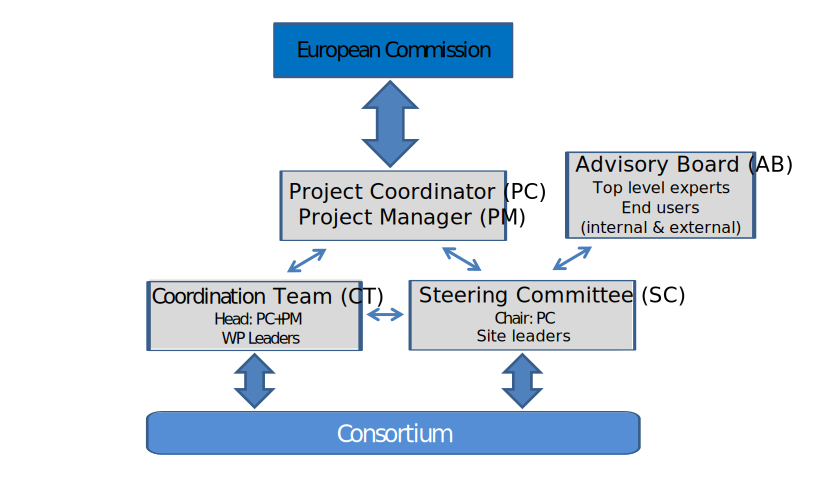
\includegraphics[width=0.75\textwidth]{management_structure.pdf}
  \caption{Management structure}
  \label{figure.management}
\end{figure}

The organisational structure, shown in the Figure~\ref{figure.management}, has been designed
to enable efficient coordination of the project --- \TODO{update}the
development and evaluation of a VRE toolkit
integrating several previously separated tools and software and
involving both academic actors and industrial stakeholders. It is jointly agreed on 
by \TheProject consortium and adapted to its size and composition, 
the tasks and duties of all partners involved. 

We have designed the management structure and procedures to deal in a
flexible manner with the following challenges:
\begin{compactitem}
\item to integrate all consortium members and to mobilise their
  expertise, knowledge and networks at every stage of the project;
\item to give the maximum attention to the end-users needs and
  requirements;
\item to continuously involve expertise and knowledge of relevant
  stakeholders and their networks, and
\item to efficiently coordinate the project implementation in a
  collaborative environment and ensure its sustainability.
\end{compactitem}

The design has been largely adapted from that of OpenDreamKit which
has proved very effective for this type of project, with some
simplification as suggested by past experience.
\begin{itemize}
\item Suppression of the Quality Review Board: its role can
  effectively be subsumed by the steering committee; also the head of
  OpenDreamKit's Quality Review Board, Hans Fanghor, will carry over
  the accumulated experience and best practices.
\item Suppression of the End User Group: as in OpenDreamKit, all
  participants are either end users themselves, or in close contact
  with such end users. To guarantee the effectiveness of this
  simplified structure, we included end users in the advisory board.
\end{itemize}


The coordinator acts as an intermediary between the Partners and
the European Commission. The coordinator will oversee the project
planning, monitor that execution is carried out in time and that
the objectives are achieved and closely interact with the project
officer for project monitoring and delivery of the performance
indicators.  The Project Manager will ensure  efficient day-to-day
management of the project, reporting, feedback to partners on
administrative, financial and legal issues, tracking of  resource
allocation and consumption, and communication inside and outside the
consortium.

The resources of all partners will be mobilised by decentralisation of
responsibilities through the assignment of leadership for work
packages. Clear distribution of tasks, efficient decision making
mechanisms and a sound financial management will safeguard the
achievement of the project's objectives.

\ifgrantagreement\else
\subsubsection{Milestones}
For a description of the milestones and their motivations see
Section~\ref{sec:milestones}; a tabulation of the milestones, which work packages
are involved, and a means of verification can be seen in Table~\ref{tab:milestonetable}.

\milestonetable
\fi

\subsubsection{Project roles}

%Project Coordinator and Project Manager can meet any time and at least
%twice a week.

The following bodies will form the organisational structure of the
\TheProject project : Coordination Team (MT), Steering Committee (SC),
Advisory Board (AB).%, End User Group (EUG) and Quality Review board (QRB).

\begin{description}
\item{\textbf{Coordination Team (CT)}} \nobreak\par
\textbf{Members:} The CT is composed of the Work Package leaders
and headed by the Project Coordinator, assisted by the Project
Manager.

\textbf{Responsibilities:} The CT is an executive body in charge of
the project implementation and monitoring.
It takes operational decisions necessary for the smooth execution of
the project.

\textbf{Tasks:}
\begin{compactenum}
\item Monitoring the timely execution of the tasks and achievement of
  the objectives;
\item Preparation of scientific and financial progress reports;
\item Controlling Work Package progress by assessing it through technical
  reports developed by the partners;
\item Making proposals to the Steering Committee of re-allocation of
  tasks, resources and financial needs for the fulfilment of the work
  plan;
\item Preparing the drafts and validating the project deliverables to
  be submitted to the Commission.
\end{compactenum}

\textbf{Meetings:} They will meet Work-Package leaders every 6 months.
If necessary, extra meetings will be arranged.

\item{\textbf{Steering Committee (SC)}}\nobreak\par

\textbf{Members:} The SC is chaired by the Project Coordinator
and includes one representative from each partner organisation.

\textbf{Responsibilities:} The SC is the decision-making body in
charge of the strategic orientation of the project.  It takes decisions on scientific
directions, re-allocation of resources, consortium
changes and intellectual property rights.

\textbf{Meetings:} Biyearly. If necessary, extra-meetings
will be arranged.  Written minutes of each meeting will be produced,
which shall be the formal record of all decisions taken. A procedure
for comment and acceptance is proposed.

\textbf{Voting procedure:} The SC shall not deliberate until a quorum
of three-fourth (3/4) of all Members are present (possibly through
video-conference) or represented. Each Member shall have one vote. The
SC will work on consensual decisions as much as possible and resort to
voting only if unavoidable. Voting decisions shall be taken by a
majority of two-thirds (2/3) of votes with quorum two-thids (2/3) of
the whole set of members. Exceptional decisions (large changes to the
budget ($\geq$ 100k euros), evolution to the consortium, firing the
coordinator, resolving ambiguity about whether something is a hard
question) shall be taken by a majority of three-fourth (3/4) of votes
with quorum three-fourth (3/4) of the whole set of members. Votes can
be electronic.

\item{\textbf{Advisory board (AB)}} \nobreak\par

  \textbf{Members:} top level experts and end-users from partner and
  external organisations, from a variety of disciplines and both from
  academic and industrial sector. Together, they have a deep
  understanding of both market and technical problems, and an
  awareness of opportunities

  \textbf{Responsibilities:} to give an independent opinion on
  steering, scientific and innovation matters, in order to guaranty
  quality implementation of the project, adequateness to the end-users
  needs, efficient innovation management, and project sustainability.

  % \textbf{Tasks:} to control the project execution from the point of
  % view of the end user needs and requirements, to test the tool and to
  % detect its potential shortcomings at the early stages, to propose
  % adaptation measures.

  \textbf{Meetings:} at the request of the Steering Committee.
\end{description}

\subsubsection{Project management tools and procedures}

Project partners and management bodies will communicate through
a dedicated project web platform, maintained by the Project
Manager. WP leaders will monitor progress of
participants of their WP at least monthly, and participants will inform their WP
leaders when problems are encountered. Major problems will be
discussed in (teleconference) meetings with the Project Coordinator
and Project Manager. Each WP leader will be free to organise
extra meetings with WP partners, if necessary. Scientific and
financial progress reports will be collected, assembled and
transmitted to the Project Coordinator by the WP leaders through the
web platform. On basis of the Progress Reports, the Coordination Team
will monitor progress of the project, identify bottlenecks and find
solutions for these problems. Where needed, adaptations to the project
plan will be made, with the aim of ensuring the delivery of the project
results as agreed with the EC. Major adaptations need to be approved
by the Steering Committee.

The Coordination Team, will ensure efficient innovation management.
They will carefully monitor new opportunities in order to suggest, if
necessary, to new directions to the Steering Committee. For legal
aspects, the latter will have a feedback from legal officers from the
Coordinator’s European Affairs and Technology Transfer office (SAIC),\TODO{Update}
specialised in Intellectual Property.

Our management structure and procedures will ensure that our network
of partners from both academic and industrial sectors is focused at
achieving the promised tasks and deliverables, efficiently managing
the innovation process and largely opening the VRE to its final users.
The partners will sign a Consortium Agreement, in which operational
rules and decision making procedures will be laid down.

\subsubsection{Risks and risk management strategy}\label{sec:risks}

The risk in the project execution as planned is carefully assessed and
managed. We base our plans on long standing experience, and we bring
together the world's experts in the relevant tools and techniques.

A key feature of this project is the involvement of a wide set of
partners from multiple domains. While this ensures complementary
coverage of a wide set of skills and provides robustness in different
ways, we will have to ensure that all partners work as closely knit
team. 

Our open source approach means that all our code and outputs
are open and visible to anybody at sites like Github and bitbucket
throughout the project. In particular, it is common for users of
computational software to use the leading edge versions, thus
beta-testing code in-between major releases. This results in risk
reduction: where our design decision or technical approaches are
controversial, this will be detected early by those users, giving the
consortium useful feedback to consider.

The project coordinator will, with support from the Coordination Team
and Quality Review Board, create a Risk Management Plan
\delivref{management}{ipr} as part of the Management Work Package,
which will be reviewed annually.
\ifgrantagreement\else
An initial risk assessment appears as figure \ref{risk-table}.

\TOWRITE{ALL}{risk about EOSC integration}

\begin{figure}
\begin{center}
\begin{tabular}{|m{.2\textwidth}|m{.12\textwidth}|m{.58\textwidth}|}\hline
  Risk & Level with / without mitigation & Mitigation measures
  \\\hline
  
   \multicolumn{3}{|c|}{
    \textit{General technical / scientific risks}
   }
   \\\hline
  
  Implementing infrastructure that does not match the needs of end users & High/Low &
  Most of the members of the consortium are themselves end-users with
  a diverse range of needs and points of views; hence the design of
  the proposal and the governance of the project is naturally steered
  by demand; besides, because we provide a toolkit, users have the
  flexibility to adapt the infrastructure to their needs.\\\hline
  
  Lack of predictability for tasks that are pursued jointly with
  the community & Medium/Low &
  The PI's have a strong experience managing community-developed
  projects where the execution of tasks depends on the availability of
  partners. Some tasks may end up requiring more manpower from
  \TheProject to be completed on time, while others may be entirely
  taken care of by the community. Reallocating tasks and redefining
  work plans is common practice needed to cater for a
  fast evolving context. Such random factors will be averaged out over
  the large number of independent tasks.\\\hline
  
  Reliance on external software components & Medium/Low & The non trivial
  software components \TheProject relies on are open source. Most are
  very mature
  and supported by an active community, which offers strong long run
  guarantees.  The critical emerging software component Jupyter
  builds on \IPython which has been around for a decade and is very
  mature. The other components could be replaced by alternatives, or
  worst comes to worst, taken over by the participants.
  \\\hline

  \multicolumn{3}{|c|}{
    \textit{Use-case risks}
  }
  \\\hline

  & & \TOWRITE{WP4}{Risks related to use-cases in WP4}
  \\\hline

  \multicolumn{3}{|c|}{
    \textit{Management risks}
  }
  \\\hline

  Recruitment of highly qualified staff & High/Medium &
  Great care was taken identifying pool of candidates to hire from,
  and coordinating with currently running projects to rehire personnel
  with strong track record. Typically, we will rehire European
  postdocs that are currently funded by the Sloan grant to work on
  Jupyter in California and wish to come back to Europe.\\\hline

  Different groups not forming effective team & Medium/Low & Long
  track record of working collaboratively on code across multiple
  sites; Aggressive planning of project meetings, work-shops and
  one-to-one partner visits to facilitate most effective teamwork,
  combining face-to-face time at one site with remote
  collaboration.\\\hline 
  % this also justifies our generous travel budget.

  Partner leaves the consortium & Low/High & If the GA requires a replacement
  in order to achieve the project's objectives, the consortium will invite a new 
  relevant partner in. If a replacement is not necessary, the resources and tasks 
  of the departing partner will be reallocated to the alternative ones within the 
  consortium.
  \\\hline

  \multicolumn{3}{|c|}{
    \textit{Dissemination risks}
  }
  \\\hline

  Impact of dissemination activities is lower than planned. & Low/Medium & 
  Partners in the consortium have a proven track record of publishing in top-level 
  scientific venues with the highest impact, which reduces the risk. The Project Coordinator 
  will monitor impact of all dissemination activities. If a deficiency is identified, the consortium 
  will propose relevant corrective actions.\\\hline

  \end{tabular}
\end{center}
\caption{\label{risk-table}Initial Risk Assessment}
\end{figure}
\fi
%\TOWRITE{NT/Eugenia}{Impredictability}

%\includegraphics[width=.94\textwidth]{Pictures/Impact-img1.png}

%   But: since Open Source softwares are freely accessible, security
%   and privacy issues are a concern. Anytime a resource is shared,
%   there is greater risk of unauthorised access and contaminated data.
%   Providers must demonstrate security solutions, which should include
%   physical security controlling access to the facility and protection
%   of user data from corruption and cyber attacks.}


\TOWRITE{ALL}{
  Add a paragraph about data management plan. What data will we produce, which data is available from the start, how do we handle it...
}

%  LocalWords:  mgt Paris-Sud UPSud Thiery Sage-Combinat decentralisation textwidth hline
%  LocalWords:  textwidth Jupyter slmhnlnhfnhs hsfhs ghshsh includegraphics unauthorised

%%% Local Variables:
%%% mode: latex
%%% TeX-master: "proposal"
%%% End:
%  LocalWords:  TOWRITE subsubsection organisational compactenum ipr Impredictability
%  LocalWords:  textbf nobreak smallbreak


\draftpage
\subsection{Consortium as a Whole}
%\TO WRITE{ALL}{Proofread 3.4 consortium pass 2 [Done by Hans]}
%remove this, as we have more pressing things left.

\eucommentary{\begin{compactitem}
\item
Describe the consortium. How will it match the project's objectives?
How do the members complement one another (and cover the value chain,
where appropriate)? In what way does each of them contribute to the
project? How will they be able to work effectively together?
\item
If applicable, describe the industrial/commercial involvement in the
project to ensure exploitation of the results and explain why this is
consistent with and will help to achieve the specific measures which
are proposed for exploitation of the results of the project (see section 2.3).
\item
Other countries: If one or more of the participants requesting EU funding
is based in a country that is not automatically eligible for such funding
(entities from Member States of the EU, from Associated Countries and
from one of the countries in the exhaustive list included in General
Annex A of the work programme are automatically eligible for EU funding),
 explain why the participation of the entity in question is essential to carrying out the project
\end{compactitem}
}

\TOWRITE{All}{Convert site names to standard abbreviations}

The BOSSEE consortium spans the broad spectrum of actors required for successfully developing an apt and easy-to-navigate sustainable service accessible through the EOSC hub catering to the needs of the European scientific community. The consortium brings in:
\begin{itemize}
\item A set of use cases that cover several application domains and users, and that impose very diverse requirements on EOSC infrastructure (XFEL, CDS ASTRO); 
\item Lead developers in of the Jupyter Ecosystem, including IPython, the Jupyter Notebook, JupyterLab, JupyterHub, Binder, MyBinder.org, IPyWidgets (name??) located at Simula, European XFEL, QuantStack and WildTreeTech [import here to have the section on "what is the Jupyter ecosystem? somewhere, so we can make reference to it ?...; 
\item Experts and major ?promoters? of the JUPYTER collaborative user interfaces for interactive and exploratory computing in a variety of scientific domains (European XFEL, QuantStack, Paris-Sued, Ecole Polytechnique, Simula, Silesia, [others?]). 
\item A long experience and proven track record of success with large and complex collaborative projects, including projects focused on large-scale infrastructures and large experimental services (EGI, XFEL?) as well as experience in running large scale open source projects (Jupyter project) 
\item A comprehensive range of skill sets and competencies in several relevant domains, from applied research to standardisation to business
analysis.
\end{itemize}

\end{compactenum}

\TOWRITE{ALL}{description of collaborations}

\TOWRITE{ALL}{Add previous collaborations}

% joint software/database development
% Jupyter Project software?

% Binder
\jointsoft{SRL,WTT}

% k3d
\jointsoft{SIL,SRL}
\jointsoft{SIL,XFEL}
\jointsoft{SRL,XFEL}

% nbval
\jointsoft{XFEL,SRL}

%% joint projects

% OpenDreamKit: UPSUD, SIL, XFEL, SRL
\jointproj{XFEL,UPSUD} joint project
\jointproj{XFEL,SRL} joint project
\jointproj{XFEL,SIL} joint project

\jointproj{UPSUD,SRL} joint project
\jointproj{UPSUD,SIL} joint project

\jointproj{SRL,SIL} joint project


% panosc
\jointproj{XFEL,EGI} joint project

% Jupyter project publication ? XXX TIM
\TODO{Add colloboration from joint Jupyter project publication (lead
  by Kluyver) ? Tim, thomas K?}
\jointpub{A,B} % some publication

%joint supervision
% \jointsup{A,B} %

%joint organization
% \jointorga{A,B} % some org
\jointorga{SA,UJF} % PASCO'15

% joint publications
% \jointpub{A,B} % some publication
\coherencetable[swsites]

%%% Local Variables:
%%% mode: latex
%%% TeX-master: "proposal"
%%% End:

%%% Local Variables:
%%% mode: latex
%%% TeX-master: "proposal"
%%% End:

\draftpage

\subsection{Resources to be Committed}\label{sec:resources}
\TOWRITE{ALL}{Proofread 3.4 pass 2 (especially first paragraph Staff efforts)}

\eucommentary{Please provide the following:
\begin{compactitem}
\item
a table showing number of person/months required (table 3.4a)
\item
a table showing 'other direct costs' (table 3.4b) for participants where
those costs exceed 15\% of the personnel costs (according to the budget
table in section 3 of the administrative proposal forms)
\end{compactitem}}

\subsubsection{Management Level Description of Resources and Budget}
\label{sect:budget-details}

\paragraph{Staff efforts}

\eucommentary{Please indicate the number of person/months over the whole
duration of the planned work, for each work package, for each participant.
Identify the work-package leader for each WP by showing the relevant
person-month figure in bold.}


\ifgrantagreement.\else{} %
displayed in the following table.
\wpfig[label=fig:staffeffort,caption=Summary of Staff Efforts]
\fi

\paragraph{Travel, dissemination, and outreach}

...

\subparagraph{Guidelines for travel and dissemination}
\label{sect:budget-details-travel}

...

\subparagraph{Guidelines for outreach costs}
\label{sect:budget-outreach-publication-charges}
...
\bigskip

\subsubsection{Resource summaries for consortium member sites}
\label{resources.summary}

%%%%%%%%%%%%%%%%%%%%%%%%%%%%%%%%%%%%%%%%%%%%%%%%%%%%%%%%%%%%%%%%
%
% Guidelines for completion of partner specific resource summary:
%
%
% Please explain how many person months for each person are
% requested. Say who is the local lead. Say anything that helps to
% understand why people are recruited as you plan, in particular if
% this deviates from having one research for 48 months.  We can also
% use this bit of the proposal (and the table, see below) to address
% any other unusual arrangements.
%
%
% The table should contain all non-staff costs (the EU requests that
% this table must be present if the non-staff costs exceed
% 15% of the total cost, but it is good practice and will show
% openness and transparency that we show the data for all partners).
%
% Link back from the table to the work packages and tasks for which
% the expenses are required. Add information that makes it easier to
% understand why the expenses are justified.
%
%     To refer to a task in a work package, use "\taskref{WP-ID}{TASK-ID}" where
%     WP-ID is the ID of the work package:
%        WP#: WP-ID - full title
%        ----------------------
%        WP1: 'management' - Management
%        WP2: 'community' - Community Building and Engagement
%        WP3: 'component-architecture' - Component Architecture
%        WP4: 'UI' - User interfaces
%        WP5: 'hpc' - High Performance Computing
%        WP6: 'dksbases' - Data/Knowledge/Software-Bases
%        WP7: 'social-aspects' - Social Aspects
%        WP8: 'dissem' - Dissemination
%
%
%     and "TASK-ID" is the ID of the task. You can set this using
%
%       \begin{task}[id=TASK-ID,title=Math Search Engine,lead=JU,PM=10,lead=JU]
%
%     To refer to deliverables, use "\delivref{WP-ID}{DELIV-ID}" where DELIV-ID is
%     the ID of the deliverable that can be set like this:
%
%       \begin{wpdeliv}[due=36,id=DELIV-ID,dissem=PU,nature=DEM]
%           {Exploratory support for semantic-aware interactive widgets providing views on objects
%           represented and or in databases}
%       \end{wpdeliv}
%
%
% The table is pre-populated with entries most sites are likely
% to need. If a line does not apply to you, just delete it. If you need
% an extra line, then add it. Use common sense: the number of rows should not
% be very big, but at the same time it is useful to give some breakdown/explanation
% of costs.
%
%
% Eventually, try to create you entry similar in style to the others.
% (The Southampton entry is fully populated, so use this as guidance
% if in doubt.)
%
%
%%%%%%%%%%%%%%%%%%%%%%%%%%%%%%%%%%%%%%%%%%%%%%%%%%%%%%%%%%%%%%%%

In this section we briefly describe the requested resources. See the
participant descriptions in the description of the consortium for the
specific role of each member.

%%%%%%%%%%%%%%%%%%%%%%%%%%%%%%%%%%%%%%%%%%%%%%%%%%%%%%%%%%%%%%%%%%%%%%%%%%%%%%
\paragraph{Resources Simula Research Laboratory}

\site{SR} requests X person months for the project coordinator, Y person months ...


\bigskip
\begin{table}[H]
\begin{tabular}{|r|r|p{8.5cm}|}
\hline
\textbf{2: \site{SR}} & \textbf{Cost (\euro)} & \textbf{Justification} \\\hline
\textbf{Travel}
  &  XXX & Travel (see the guidelines \ref{sect:budget-details-travel})\\\hline
\textbf{Publication charges}
  &   XXX & Open access publication charges (see \ref{sect:budget-outreach-publication-charges})\\\hline
%%\textbf{Equipment}
%%  &   0 &  \\\hline    %\taskref{WP-ID}{TASK-ID}
\textbf{Other goods and services}
  & XXX &
 \\\hline   %\taskref{WP-ID}{TASK-ID} \delivref{WP-ID}{DELIV-ID}
\textbf{Total}
 & XXX\\\cline{1-2}
\end{tabular}
\caption{Overview: Non-staff resources to be committed at CNRS (all in \texteuro)}\vspace*{-1em}
\end{table}

%%%%%%%%%%%%%%%%%%%%%%%%%%%%%%%%%%%%%%%%%%%%%%%%%%%%%%%%%%%%%%%%%%%%%%%%%%%%%%
\paragraph{Resources Facility}

\site{...} requests
X person months for

\taskref{wpid}{taskid}


\bigskip
\begin{table}[H]
\begin{tabular}{|r|r|p{8.5cm}|}
\hline
\textbf{2: \site{SR}} & \textbf{Cost (\euro)} & \textbf{Justification} \\\hline
\textbf{Travel}
  &  XXX & Travel (see the guidelines \ref{sect:budget-details-travel})\\\hline
\textbf{Publication charges}
  &   XXX & Open access publication charges (see \ref{sect:budget-outreach-publication-charges})\\\hline
%%\textbf{Equipment}
%%  &   0 &  \\\hline    %\taskref{WP-ID}{TASK-ID}
\textbf{Other goods and services}
  & XXX &
 \\\hline   %\taskref{WP-ID}{TASK-ID} \delivref{WP-ID}{DELIV-ID}
\textbf{Total}
 & XXX\\\cline{1-2}
\end{tabular}
\caption{Overview: Non-staff resources to be committed at CNRS (all in \texteuro)}\vspace*{-1em}
\end{table}


% ---------------------------------------------------------------------------
%  Section 4: Members of the Consortium
% ---------------------------------------------------------------------------

\newpage

\eucommentary{This section is not covered by the page limit.\\
The information provided here will be used to judge the operational capacity.}

\section{Members of the Consortium}
\TOWRITE{ALL}{Proofread 4. Members of the consortium pass 2}

\subsection{Participants}

\eucommentary{Please provide, for each participant, the following (if available):\\
\begin{compactitem}
\item
a description of the legal entity and its main tasks,
with an explanation of how its profile matches the tasks in the proposal;
\item
a curriculum vitae or description of the profile of the persons,
including their gender, who will be primarily responsible for carrying
out the proposed research and/or innovation activities;
%
this includes a description of the profile of the to-be-recruited personnel
\item
a list of up to 5 relevant publications, and/or products, services
(including widely-used datasets or software), or other achievements
relevant to the call content;
\item
a list of up to 5 relevant previous projects or activities, connected
to the subject of this proposal;
\item
a description of any significant infrastructure and/or any major items
of technical equipment, relevant to the proposed work;
\item
any other supporting documents specified in the work programme for this call.
\end{compactitem}}

\begin{sitedescription}{SRL}

Dedicated to tackling scientific challenges with long-term impact and of genuine importance to real life, Simula Research Laboratory (Simula) offers an environment that emphasises and promotes basic research. At the same time, we are deeply involved in research education and application-driven innovation and commercialisation.

Simula was established as a non-profit, limited company in 2001, and is fully owned by the Norwegian Ministry of Education and Research. Its research is funded through competitive grants from national funding agencies and the EC, research contracts with industry, and a basic allowance from the state.  Simula's operations are conducted in a seamless integration with the two subsidiaries Simula School of Research and Innovation and Simula Innovation.

At its outset, the laboratory was given the mandate of becoming an internationally leading research institution within select fields in information and communications technology. These fields are (i) communication systems, including cyber-security; (ii) scientific computing, aiming at fast and reliable solutions of mathematical models in biomedicine, geoscience, and renewable energy; and (iii) software engineering, focusing on testing and verification of mission-critical software systems, and on planning and cost estimation of large software development projects. Recent evaluations state that Simula has met its challenge and is an acknowledged contributor to top-level research in its focus areas. Specifically, in the 2012 national evaluation of ICT research organised by the Research Council of Norway and conducted by an international expert panel, Simula received the highest average score (4.67) on a 1-5 scale among all evaluated institutions.  In comparison, the national average was 3.38. Only five of the 62 research groups evaluated were awarded the top grade (5), and two of these five groups are located at Simula.

Simula has hosted one Norwegian Centre of Excellence, Centre for Biomedical Computing (2007-2017), and one Norwegian Centre for Research-based Innovation, Certus (2011-2018). In addition, we participate as research partner in another Centre for Research-based Innovation, Centre for Cardiological Innovation (2011-2018), hosted by Oslo University Hospital. These two centre-oriented schemes are the most prestigious funding instruments offered by the Research Council of Norway.

\subsubsection*{Curriculum vitae}

% Curriculum of the personnel at this institution

\begin{participant}[type=PI,PM=28,gender=male]{Benjamin Ragan-Kelley}
  % PM=YYY:
  % A fair evaluation of the number of months you will be
  % spending on this specific project along the four years.
  % Typical numbers:
  % - full time hired personnel: 48 months
  % - lead PI or proposal coordinator: 8-12 months
  % - PI: 4-5 months
  % - participant: 2-6 months

  % salary=ZZZ:
  % Approximate monthly gross salary (in term of total cost for the
  % employer). This is optional. If you are uncomfortable having this
  % information in a public file, you can alternatively send the
  % information to Eugenia Shadlova, or to your institution
  % leader/manager if he is willing to fill in himself the budget
  % forms on the eu portal.

Benjamin Ragan-Kelley is one of the core maintainers and developers
of the Jupyter and IPython projects, and currently leads the JupyterHub
and BinderHub development teams.
He has been a contributor to these projects since 2006,
prior to the establishment of Jupyter as a separate project from IPython.
He is an expert in all levels of Jupyter development,
especially the aspects of deploying Jupyter-based services,
which is the focus of this proposal.
Benjamin will lead \TheProject.

Beyond Jupyter, Benjamin has contributed widely to open source software,
especially in the scientific Python community.
He is a maintainer of numerous scientific packages
in the conda-forge package management system,
building packages used widely in education and research,
such as PETSc, MPICH, and FEniCS.

Benjamin is a Research Engineer in the department of Scientific Computing and Numerical Analysis
at Simula Research Laboratory in Oslo, Norway,
where his primary responsibility is developing and maintaining the Jupyter software ecosystem,
as well as supporting research scientists in diverse fields,
including biomedical computing.

Prior to his current position at Simula,
Benjamin received his Bachelor's degree \textit{Magne cum Laude} in Engineering Physics in 2007
from Santa Clara University and his PhD in Applied Science and Technology
from the University of California, Berkeley in 2013.
He worked as a postdoctoral fellow at Simula Research Laboratory prior
to becoming a permanent Research Engineer.
He was honored along with the rest of the Jupyter steering council
with the 2017 ACM Software System Award for Jupyter.


\end{participant}

%%% Local Variables:
%%% mode: latex
%%% TeX-master: "../proposal"
%%% End:

% \input{CVs/Simula-not-known.tex}
% \input{CVs/First.Last.tex}

\subsubsection*{Publications, products, achievements}

\begin{compactenum}
\item 2017 ACM Software System Award for Jupyter
\item M. Bussonier, J. Forde, J. Freeman, B. Granger, T. Head, C. Holdgraf, K. Kelley, G. Nalvarte, A. Osheroff, M. Pacer et al. Binder 2.0 - Reproducible, interactive, sharable environments for science at scale In Python in Science ConferenceProceedings of the 17th Python in Science Conference. Austin, Texas: SciPy, 2018.
\item J. Forde, T. Head, C. Holdgraf, Y. Panda, G. Nalvarte, M. Pacer, F. Perez, B. Ragan-Kelley and E. Sundell. Reproducible Research Environments with Repo2Docker In ICML 2018 Reproducible Machine Learning. ICML, 2018.
\item T. Kluyver, B. Ragan-Kelley, F. Perez, B. Granger, M. Bussonier, J. Frederic, K. Kelley, J. Hamrick, J. Grout, S. Corlay et al. Jupyter Notebooks: a publishing format for reproducible computational workflows In 20th International Conference on Electronic Publishing. IOS Press, 2016.

\end{compactenum}

\subsubsection*{Previous projects or activities}

\begin{compactenum}
\item OpenDreamKit -
\item Jupyter - collaboration with UC Berkeley, Cal Poly, funded by Gordon \& Betty Moore Foundation,
      Alfred P. Sloan Foundation, and Helmsley Trust
\item Binder - collaboration with UC Berkeley, funded by Gordon \& Betty Moore Foundation
\end{compactenum}

\subsubsection*{Significant infrastructure}

The fully owned Simula subsidiary Simula Innovation handles pre-commercial innovation projects, creation and follow-up of company spin-offs, and general support for entrepreneurs.

\end{sitedescription}



%KEY-MORE-TODOS


%%% Local Variables:
%%% mode: latex
%%% TeX-master: "../proposal"
%%% End:

%  LocalWords:  sitedescription Simula Simula commercialisation Certus subsubsection Logg
%  LocalWords:  Mardal Funke Rognes Sci Comput Langtangen FEniCS Aln ae lgaard vspace
%  LocalWords:  TOWRITE emphasises organised

\clearpage
\begin{sitedescription}{XFEL}
  \label{sitedescription:euxfel}

% PIC:
% see: http://ec.europa.eu/research/participants/portal/desktop/en/orga

% See ../proposal.tex, section Members of the Consortium for a
% complete description of what should go there

  European X-Ray Free-Electron Laser Facility GmbH is a limited
  liability company under German law. At present, 12 countries are
  participating in the project: Denmark, France, Germany, Hungary,
  Italy, Poland, Russia, Slovakia, Spain, Sweden, Switzerland, and the
  United Kingdom.  The company is in charge of the operation and
  construction of the European XFEL, a 3.4 km long X-ray free-electron
  laser facility extending from Hamburg to the neighbouring town of
  Schenefeld in the German federal state of Schleswig-Holstein. Civil
  construction started in early 2009, and the user operation in
  September 2017. With its repetition rate of 27,000 pulses per second
  and a peak brilliance a billion times higher than that of the best
  synchrotron X-ray radiation sources, the European XFEL will allow
  the investigation of still open scientific problems in a variety of
  disciplines (physics, structural biology, chemistry, planetary
  science, study of matter under extreme conditions and many others).


\subsubsection*{Curriculum vitae}

% Curriculum of the personnel at this institution
%
\begin{participant}[type=leadPI,PM=4,gender=male]{Hans Fangohr}
  % type is one of:
  % - leadPI: leader of the participating institution
  % - PI: Principal Investigator
  % - R: researcher?
  % Who is the coordinator is specified elsewhere

  % PM=YYY:
  % A fair evaluation of the number of months you will be
  % spending on this specific project along the four years.
  % Typical numbers:
  % - full time hired personnel: 48 months
  % - lead PI or proposal coordinator: 8-12 months
  % - PI: 4-5 months
  % - participant: 2-6 months

  % salary=ZZZ:
  % Approximate monthly gross salary (in term of total cost for the
  % employer). This is optional. If you are uncomfortable having this
  % information in a public file, you can alternatively send the
  % information to Eugenia Shadlova, or to your institution
  % leader/manager if he is willing to fill in himself the budget
  % forms on the eu portal.

  % The above information is used to fill in various tables in the
  % proposal file, and to evaluate the cost of the project for the
  % institutions.

  % You may remove all those comments.

  % About half a page of free text; for whatever it's worth, you may see
  % Nicolas.Thiery.tex for an example.



  \medskip Hans Fangohr is an academic at the University
  of Southampton in the United Kingdom since 2002 (full professor
  since 2010), and leading the data analysis services at European XFEL
  in Germany since 2017.

  He has been a long term proponent of Open Science, and in particular
  involved with the the use and further development of the Jupyter
  Notebook to enable this. He has hosted Thomas Kluyver at the
  University of Southampton since 2015 from where he contributed as a
  core developer of the Jupyter team. As a PI in the EC-funded e-INFRA
  OpenDreamKit project (2015-2019), he has pushed forward the use of
  Jupyter Notebooks for reproducible computational science, and
  started the notebook validation tool (NBVAL). He made use of the
  Jupyter Ecosystem for research and education at graduate and
  postgraduate level at the University of Southampton, and shared
  resources widely, including a text book provided through Jupyter
  Notebooks, which can be executed interactively online [1].

  Since 2017, he is designing data analysis services and
  infrastructure at the European XFEL research facility. European XFEL
  is using IPython and the Jupyter Notebook as core utilities in their
  large scale experiment control, data capture and data
  analysis. Within the e-INFRA project PaNOSC (Photon and Neutron
  Science Open Cloud, 2018-2021), he is leader of the Work Package 4,
  which is focused on data analysis services for the EOSC Hub, and the
  use of the Jupyter notebook with its existing features on the EOSC
  hub.

  In this project (BOSSEE), where new capabilities for the Jupyter
  notebook and ecosystem are being designed, Hans' wide experience and
  interaction with different science groups will be beneficial to
  ensure the outcome is of value to open science in many domains. This
  includes him chairing the interdisciplinary computational modelling
  group at the University of Southampton (200 academics, 2008-2017),
  chairing the national EPSRC scientific advisory committee on High
  Performance Computing in the UK (2014-2017) and interacting with a
  large variety of science users at European XFEL in his role
  to lead the data analysis service provision.
\end{participant}

%%% Local Variables:
%%% mode: latex
%%% TeX-master: "../proposal"
%%% End:

\begin{participant}[type=PI,PM=1,gender=male]{Sandor Brockhauser}
  % type is one of:
  % - leadPI: leader of the participating institution
  % - PI: Principal Investigator
  % - R: researcher?
  % Who is the coordinator is specified elsewhere

  % PM=YYY:
  % A fair evaluation of the number of months you will be
  % spending on this specific project along the four years.
  % Typical numbers:
  % - full time hired personnel: 48 months
  % - lead PI or proposal coordinator: 8-12 months
  % - PI: 4-5 months
  % - participant: 2-6 months

  % salary=ZZZ:
  % Approximate monthly gross salary (in term of total cost for the
  % employer). This is optional. If you are uncomfortable having this
  % information in a public file, you can alternatively send the
  % information to Eugenia Shadlova, or to your institution
  % leader/manager if he is willing to fill in himself the budget
  % forms on the eu portal.

  % The above information is used to fill in various tables in the
  % proposal file, and to evaluate the cost of the project for the
  % institutions.

  % You may remove all those comments.

  % About half a page of free text; for whatever it's worth, you may see
  % Nicolas.Thiery.tex for an example.


  \medskip

  Sandor Brockhauser is the head of the Control and Analysis Software
  Group at the European XFEL. He received his M.Sc. in Informatics
  from Technical University of Budapest, Hungary, earned a Ph.D. from
  University of Leoben, Austria, and received his HDR degree in
  physics at the University of Joseph Fourier, Grenoble in
  France.

  Since 2004, when he joined the European Molecular Biology
  Laboratory (EMBL) in Grenoble, France, he worked in Macromolecular
  Crystallography and became the scientist in charge of the Multi-
  Wavelength Anomalous Dispersion Beamline ID14-4 at European
  Synchrotron Radiation Facility (ESRF), France. Between 2013-15, he
  moved to Szeged, Hungary where he joined the Extreme Light
  Infrastructure, ELI-ALPS, and has established and built up its
  Scientific Engineering Division. In the same time, he also
  established the X-ray Crystallography Laboratory at a European
  Center of Excellence, the Biological Research Center, Szeged of the
  Hungarian Academy of Sciences. Moving to the European XFEL in 2016,
  he became responsible for the full control system of the beamlines
  and scientific instruments, Karabo, that enables the integration of
  Experiment Control, Data Acquisition and Analysis. During the last
  two years, Karabo has been deployed, photon beamlines were
  successfully commissioned and two of the initial scientific
  instruments have been put in operation producing 0,5PT of data in 5
  weeks of experiments. Jupyter tools are embedded in the Karabo
  system and European XFEL analysis activities.

\end{participant}

%%% Local Variables:
%%% mode: latex
%%% TeX-master: "../proposal"
%%% End:

\begin{participant}[type=leadPI,PM=1,gender=male]{Krzysztof Wrona}
  % type is one of:
  % - leadPI: leader of the participating institution
  % - PI: Principal Investigator
  % - R: researcher?
  % Who is the coordinator is specified elsewhere

  % PM=YYY:
  % A fair evaluation of the number of months you will be
  % spending on this specific project along the four years.
  % Typical numbers:
  % - full time hired personnel: 48 months
  % - lead PI or proposal coordinator: 8-12 months
  % - PI: 4-5 months
  % - participant: 2-6 months

  % salary=ZZZ:
  % Approximate monthly gross salary (in term of total cost for the
  % employer). This is optional. If you are uncomfortable having this
  % information in a public file, you can alternatively send the
  % information to Eugenia Shadlova, or to your institution
  % leader/manager if he is willing to fill in himself the budget
  % forms on the eu portal.

  % The above information is used to fill in various tables in the
  % proposal file, and to evaluate the cost of the project for the
  % institutions.

  % You may remove all those comments.

  % About half a page of free text; for whatever it's worth, you may see
  % Nicolas.Thiery.tex for an example.



  \medskip Krzysztof Wrona has a background in computer physics. As
  the group leader of IT and Data Management at European XFEL, he is
  in charge of the management of scientific data in the frame of the
  user program of the European XFEL facility. He has more than 15
  years of experience in data storage, processing, and in general IT
  issues.
\end{participant}

%%% Local Variables:
%%% mode: latex
%%% TeX-master: "../proposal"
%%% End:

\begin{participant}[type=R,PM=48,gender=male]{Thomas Kluyver}
  % PM=YYY:
  % A fair evaluation of the number of months you will be
  % spending on this specific project along the four years.
  % Typical numbers:
  % - full time hired personnel: 48 months
  % - lead PI or proposal coordinator: 8-12 months
  % - PI: 4-5 months
  % - participant: 2-6 months

  % salary=ZZZ:
  % Approximate monthly gross salary (in term of total cost for the
  % employer). This is optional. If you are uncomfortable having this
  % information in a public file, you can alternatively send the
  % information to Eugenia Shadlova, or to your institution
  % leader/manager if he is willing to fill in himself the budget
  % forms on the eu portal.
  Thomas Kluyver is one of the core maintainers of the Jupyter and IPython
  projects, which form a central part of this proposal.
  He has been part of the core IPython development team since 2011,
  before Jupyter was split out as a separate project.
  He is closely familiar with key parts of the code, and was one of
  15 core developers to receive the 2017 ACM Software System Award.

  Besides Jupyter, Thomas has contributed to a wide range of open source
  software projects in the Python ecosystem, ranging from other scientific
  computing tools such as h5py to packaging utilities such as Flit, as well
  as improvements in the Python standard library.

  Thomas is part of the Data Analysis team at European XFEL.
  He has a specific remit to facilitate the use of Jupyter by internal groups
  and visiting researchers,
  but he also contributes to the general software engineering effort working to
  allow convenient, reproducible analysis of data collected at European XFEL.

  Before working as a software engineer, Thomas studied plant biology, gaining
  a PhD from the University of Sheffield in 2013. His work since then has
  continued in close connection with research, at the University of California,
  Berkeley, and the University of Southampton, before joining European
  XFEL.
\end{participant}

%%% Local Variables:
%%% mode: latex
%%% TeX-master: "../proposal"
%%% End:

%


\begin{participant}[PM=68, type=R]{NN}

We will hire two postdoctoral-level research software engineers (for 68 person
months in total) to carry out the required work for this projet at
European XFEL. They will work under supervision of Hans Fangohr, with
support from Sandor Brockhauser and Krzysztof Wrona for particular
aspects. The employees will either have a scientific background and
significant software engineering expertise, or an education in
computer science and an aptitude to work with scientists on
computational science and data science problems.
\end{participant}

\subsubsection*{Publications, products, achievements}

\begin{compactenum}
\item H.Fangohr, Python for Computational Science and Engineering
  (2018) DOI: 10.5281/zenodo.1411868 \newline
  https://github.com/fangohr/introduction-to-python-for-computational-science-and-engineering
\item H.Fangohr et al., “Data Analysis support in Karabo at European
  XFEL”, Proceedings of International Conference on Accelerator and
  Large Experimental Physics Control Systems 2017, ISBN 978-3-95450-
  193-9, Data Analytics, Barcelona, Spain, TUCPA01 (2017) DOI: 10.18429/JACoW-ICALEPCS2017-TUCPA01
\item H.Fangohr.
\emph{A Comparison of \software{C}, \Matlab and \Python as Teaching Languages in Engineering}
Lecture Notes on Computational Science \textbf{3039}, 1210-1217 (2004)
\item T. Kluyver, B. Ragan-Kelley, F. Perez, B. Granger, M. Bussonier, J. Frederic, K. Kelley, J. Hamrick, J. Grout, S. Corlay et al. Jupyter
\emph{Notebooks: a publishing format for reproducible computational workflows} In 20th International Conference on Electronic Publishing. IOS Press, 2016.
\end{compactenum}

\subsubsection*{Previous projects or activities}

\begin{compactenum}
\item OpenDreamKit (GA No. 676541) Open Digital Research Environment
  Toolkit for the Advancement of Mathematics, participant
\item EOSCpilot (GA No. 739563) The European Open Science Cloud for
  Research Pilot Project, participant
\item PaNOSC (GA No. 823852) Photon and Neutron Open Science Cloud, participant
\end{compactenum}

\end{sitedescription}



%KEY-MORE-TODOS



%%% Local Variables:
%%% mode: latex
%%% TeX-master: "../proposal"
%%% End:

%  LocalWords:  sitedescription Programme organisations programmes Centres subsubsection
%  LocalWords:  micromagnetic Nmag Fischbacher Franchin Bordignon Fangohr emph textbf
%  LocalWords:  Multiphysics summarised Iridis TFlops Modelling

\clearpage
\begin{sitedescription}{UPSUD} \label{desc:ParisSud}

Université Paris-Sud is among the 40 top universities worldwide in the
2013 Shanghai ranking, and is one of the top two French research
universities. With about 27000 students, 1800 permanent faculty
and 1300 permanent research scientists from national research
organisations (CNRS, Inserm, INRA, Inria), it is the largest campus in
France. Since 2006, scientists from the University were awarded two
Fields medals, one Nobel Prize and a number of other national and international prizes
(European Inventor Award 2013, Wolf Prize 2010, Holweck Prize 2009,
Japan prize 2007).  Université Paris-Sud offers a
wide range of qualifications, from the exact sciences to life and health
sciences (including medical practice), legal sciences and economics. 
Research at Université Paris-Sud is an essential part of academic understanding 
and includes research activities with high commercial potential. 
Research contracts and partnership with companies make
Université Paris-Sud a key actor and a major player in French
research.  The University is located partly on the Plateau de Saclay,
the largest cluster of public and private R\&D institutions in France
(with ca. 16000 research staff), and is one of the core members of 
University Paris-Saclay – a world-class university and a
world-renowned research and innovation hub.

In the context of this project, Université Paris-Sud is the
home of one of the largest group of \Sage developers worldwide.
It is a member of the Open Source Thematic Group of the Systematic
Paris Region Systems and ICT Cluster. 
The University also hosts a major research group in Human-Centered Computing
and manages the Digiscope network of high-end visualisation platforms,
which will provide critical assets to the project.

\subsubsection*{Curriculum vitae of the investigators}

\begin{participant}[type=PI,PM=2,gender=male]{Michel Beaudouin-Lafon}

Michel Beaudouin-Lafon (PhD, Université Paris-Sud) is a Professor of Computer Science, classe exceptionnelle, 
at Université Paris-Sud and a senior fellow of Institut Universitaire de France. 
His research interests include fundamental aspects of interaction, novel interaction techniques, 
computer-supported cooperative work and engineering of interactive systems. 
He has published over 180 papers and is a member of the ACM SIGCHI Academy. 
He is the laureate of an ERC Advanced Grant exploring instrumental interaction and information substrates. 
Michel was director of LRI, the laboratory for computer science joint between Université Paris-Sud and CNRS. 
He now heads the Human-Centered Computing lab at LRI and chairs the Computer Science department at Université Paris-Saclay. 
He was Technical Program Co-chair for CHI 2013 (3500 participants), sits on the editorial boards of ACM Books and ACM TOCHI, 
and has served on many ACM committees. He received the ACM SIGCHI Lifetime Service Award in 2015.

\end{participant}

%%% Local Variables:
%%% mode: latex
%%% TeX-master: "../proposal"
%%% End:

\begin{participant}[type=PI,PM=2,gender=female]{Viviane Pons}
  Maître de Conférences at the Laboratoire de Recherche en Informatique, Viviane Pons is a
  young researcher in Algebraic Combinatorics. She defended her thesis in 2013 and has 4
  papers in international journals and 6 communications in international
  conferences, including a talk at PyCon US 2015. She was also invited as a keynote speaker
  at Pycon FR 2018. Since January 2019, she is in the editorial board of the Journal of Open Source Software.
  Before starting her research career,
  she worked for two years in industry as a Java and web developer.

  She discovered \Sage during her first \Sage Days in 2010 and has since been an active user
  and contributor with 10 (co)authored tickets improving the support of combinatorial
  objects in \Sage. She is heavily involved in the promotion of \Sage, participating in
  \Sage Days and running \Sage introduction tutorials or \Sage presentations at various
  conferences. She has also been involved in devloping the project \software{FindStat}
  dedicated to databases in combinatorics.

  Viviane is leading the very successful Community Building and
  Dissemination work package of the European Research Infrastructures
  project OpenDreamKit (2015-2019), in which 66 events (development
  workshops, training sessions, ...) were organized or coorganized,
  with more than a thousand trainees. Viviane herself organized or
  coorganized several of them, including two week-long workshops
  dedicated to women (one in 2017 and one to come in spring 2019).
\end{participant}
%%% Local Variables:
%%% mode: latex
%%% TeX-master: "../proposal"
%%% End:

\begin{participant}[type=leadPI,PM=4,gender=male]{Nicolas M. Thiéry}
  Professor at the Laboratoire de Recherche en Informatique, Nicolas M. Thiéry is a senior
  researcher in Algebraic Combinatorics with 18 papers published in international
  journals. Among other things, he is a member of the permanent committee of FPSAC, the
  main international conference of the domain, and has collaborators
  in the US and Canada where he cumulatively spent more than three
  years (Colorado School of Mines, UC Davis, Providence, Montréal),
  and India. He also
  co-organised fourteen international workshops, in particular \Sage Days, and the semester
  long program on ``Automorphic Forms, Combinatorial Representation Theory and Multiple
  Dirichlet Series'' hosted in Providence (RI, USA) by the Institute for Computational and
  Experimental Research in Mathematics.

  Algebraic combinatorics is a field at the frontier between mathematics and computer
  science, with heavy needs for computer exploration. Pioneer in community-developed open
  source software for research in this field, Thiéry founded in 2000 the \SageCombinat
  software project (incarnated as \MuPADCombinat until 2008); with 50 researchers
  in Europe and abroad, this project has grown under
  his leadership to be one of the largest organised community of Sage developers, gaining
  a leading position in its field, and making a major impact on one hundred
  publications\footnote{\url{http://sagemath.org/library-publications-combinat.html},
    \url{http://sagemath.org/library-publications-mupad.html}}. Along the way,
%this occasion
%Thiéry gained a strong community building experience, and
  he coauthored part of the proposal for NSF \SageCombinat grant
  OCI-1147247, and co-organised or taught at a dozen training and
  dissemination actions (workshops, summer schools, etc.), in
  America, Africa, Europe, and India.

  With 150 tickets (co)authored and as many refereed, Thiéry is himself a core \Sage
  developer, with contributions including key components of the \Sage infrastructure
  (e.g. categories), specialised research libraries (e.g. root systems), thematic
  tutorials, and two chapters of the book ``Calcul Mathématique avec \Sage''
  and its English translation.

  Based on this experience, and to tackle the pressing funding needs
  in the ecosystem of open source mathematical software, Thiéry
  initiated and lead the European Research Infrastructures project
  OpenDreamKit \#676541 (2015-2019, 15 sites, 50 participants, 8M€),
  engaging the Jupyter project on board. This in turn increased his
  involvement in using, promoting, and contributing to Jupyter, for
  use in mathematics and education.
\end{participant}
%%% Local Variables:
%%% mode: latex
%%% TeX-master: "../proposal"
%%% End:


\begin{participant}[type=res,PM=21]{NN}
  We will hire a full time experienced software developer to work on
  task~\taskref{math-widgets} and~\taskref{helpdesk} %longtaskref
  under the leadership of Nicolas M. Thiéry.

  The fellow will have a strong software engineering and web
  development experience, ideally in the Python, Javascript, and/or
  Jupyter ecosystem. We further require good communication and team
  working skills, in particular to work in tight collaboration with
  international open-source developer communities.
\end{participant}

\begin{participant}[type=res,PM=12]{NN}
  We will hire a full time experienced software developer to work
  on task~\taskref{collaboration} %longtaskref
  under the leadership of Michel Beaudouin-Lafon.

  The fellow will have a strong software engineering and web
  development experience (HTML/CSS/Javascript), and ideally 
  good knowledge of the Python/Jupyter ecosystems
  and/or collaboration technologies. 
  We further require good communication and team
  working skills, in particular to work in tight collaboration with
  international open-source developer communities.
\end{participant}

% Participation:
% NT: Project Management: 4PM, Component Architecture: 4PM,
%     Training/Dissemination: 2PM, User Interfaces: 2PM
% Dev 1: Component Architecture: 48PM
% Dev 2: User Interface: 24PM, CA: 10PM, HPC: 2PM
% Florent: HPC: 4PM, User Interface: 2PM (Sphinx & co)
% Viviane: Training/Dissemination: 6PM
% Loic: Training/Dissemination: 3PM, User Interfaces: 2PM
% Sam: Training/Dissemination: 6PM
% Project manager: Project management: 24PM
% PHD: ???
% Total:

\subsubsection*{Publications, achievements}

\begin{compactenum}
\item Leadership of the \SageCombinat software project.
\item Coauthoring of the open source book ``Calcul Mathématique avec
  Sage'' and its English translation , the first of its kind
  comprehensive introduction to computational mathematics in \Sage for
  education.
\item Contribution of more than 500 tickets to \Sage.
\item
Michel Beaudouin-Lafon, Olivier Chapuis, James Eagan, Tony Gjerlufsen, Stéphane Huot, Clemens Klokmose, Wendy Mackay, Mathieu Nancel, Emmanuel Pietriga, Clément Pillias, Romain Primet, Julie Wagner (2012). Multi-surface Interaction in the WILD Room, \emph{IEEE Computer}, 45(4):48–56. IEEE Computer Society.
\item
Klokmose, C.N., Eagan J.R., Baader, S., Mackay, M. and Beaudouin-Lafon, M. (2015) Webstrates: Shareable Dynamic Media. In \emph{Proceedings of the 28th annual ACM symposium on User interface software and technology (UIST ’15)}. ACM.
\end{compactenum}

\subsubsection*{Relevant projects or activities}

\begin{compactenum}
\item OpenDreamKit (GA No. 676541) Open Digital Research Environment
  Toolkit for the Advancement of Mathematics, \textbf{coordination}.
\item Hosting or coorganisation of dozens of Sage Days (week-long training and development workshops).
\item \TODO{This is not a ``previous'' project''}
Ongoing ERC Advanced Grant ONE ``Unified Principles of Interaction'' (PI: Michel Beaudouin-Lafon) that develops new user interface concepts, in particular for multi-user, multi-device environments.
\end{compactenum}

\subsubsection*{Significant infrastructure}

\site{UPSUD} hosts a local OpenStack based cloud infrastructure
\software{Cloud@VD} (400 cores) for its personnel. The participants
are regular users of this infrastructure, and in close contact with
its maintainers. As a continuation of the existing deployment of a
JupyterHub service on this infrastructure, \software{Cloud@VD} will be
available to the participants as test bed for deploying Jupyter based
services (see e.g. \taskref{eosc}{jh-bh-deployment}).

\site{UPSUD} also manages the Digiscope (\url{http://digiscope.fr}) network of high-end visualisation platforms and hosts the \software{WILD} and \software{WILDER} platforms, two ultra-high resolution wall-sized displays with motion capture and touch input for conducting research on collaborative human-computer interaction and visualisation of
large datasets.

\end{sitedescription}



\begin{draft}
\vspace{1cm}\TOWRITE{VP}{Complete check list below -- delete completed items if you wish}

\begin{verbatim}
- [ ] checked that sum of person months put into finance request is
  the same as sum of person months associated with the Work Packages
  (in proposal.tex, as defined as part of the \begin{workpackage}"
  command.

  Take into account person months associated with work package 1, time
  of all staff to be hired and work on the project (including
  investigators). Figure 5 helps with a quick check of the sums over
  different work packages.

- [X] completed site specific resource summary in resources.tex,
  including table of non-staff costs. This is compulsory (EU
  regulations) if the non-staff cost exceed 15% of the total cost, and
  is likely to be the case for most of the partners. We ask everybody
  to do it, to be consistent and show transparently how we have
  planned our total budget.

- [X] Have all our tasks a designated lead institution? Check in the
  Work Packages that all the tasks you are involved in have a
  dedicated lead party. If the lead party is "USO", then use:
  \begin{task}[lead=USO]

- [ ] Have all our deliverables a designated lead institution [using
  the 'lead=' key]?

- [X] In the "Members of the consortium section", have we addressed "a
  description of the legal entity and its main tasks, with an
  explanation of how its profile matches the tasks in the
  proposal"? See Entry for Paris-Sud and Southampton as examples.

- [X] In the Members of the consortium section, have we given
  descriptions of all the people we intend to hire (even if we don't
  know who that is yet).

- [ ] Do all our tasks include us in the list of sites involved?
\end{verbatim}
\end{draft}

%KEY-MORE-TODOS


%%% Local Variables:
%%% mode: latex
%%% TeX-master: "../proposal"
%%% End:

%  LocalWords:  sitedescription Paris-Sud organisations Inserm Inria Holweck valorisation
%  LocalWords:  Saclay subsubsection faut formel des projets antérieurs Acronyme titre
%  LocalWords:  agence financement durée Pareil les publi année SageCombinat Calcul avec
%  LocalWords:  Mathématique Logilab Sud texttt Stratuslab Chapuis

\clearpage
\begin{sitedescription}{QS}

\par QuantStack was founded in 2016 by a team of developers and maintainers of key packages of the open-source scientific computing stack. QuantStack provides support and custom development services in the Jupyter and Scientific Python ecosystems. Clients and partners of QuantStack range from financial software companies to robotics startups and public research institutions. The team comprises several core developers of Jupyter subprojects and authors of popular scientific computing and visualization software used in both academic and industrial contexts.

\par Beyond Project Jupyter, projects developed at QuantStack include data visualization packages for Jupyter such as bqplot, ipyvolume, ipyleaflet, and ipysheet, as well as Jupyter language kernels such as xeus-cling and xeus-python, and JupyterLab extensions like te draw.io and sidecar. QuantStack is also behind the development of the xtensor framework, a high-level array computing library and C++ dataframe.

\subsubsection*{Curriculum vitae of the investigators}

\begin{participant}[type=leadPI,PM=6,gender=male]{Sylvain Corlay}
  % PM=YYY:
  % A fair evaluation of the number of months you will be
  % spending on this specific project along the four years.
  % Typical numbers:
  % - full time hired personnel: 48 months
  % - lead PI or proposal coordinator: 8-12 months
  % - PI: 4-5 months
  % - participant: 2-6 months

  % salary=ZZZ:
  % Approximate monthly gross salary (in term of total cost for the
  % employer). This is optional. If you are uncomfortable having this
  % information in a public file, you can alternatively send the
  % information to Eugenia Shadlova, or to your institution
  % leader/manager if he is willing to fill in himself the budget
  % forms on the eu portal.
  Sylvain Corlay is the founder and CEO of QuantStack. He holds a PhD in applied mathematics from University Paris VI.

  As an open source developer, Sylvain contributes to Project Jupyter in the area of interactive widgets for the notebook, and is steering committee member of the Project. He also serves as a member of the board of directors for the NumFOCUS foundation, and co-organizes the PyData Paris Meetup, a regular seminar series on open-source scientific computing.

  Sylvain was one of the 15 core Jupyter developers to receive the 2017 ACM Software System Award.

  Besides Jupyter, Sylvain authors and contributes to a number of scientific computing open-source projects such as bqplot, xtensor and ipyleaflet.

  Prior to founding QuantStack, Sylvain was a quant researcher at Bloomberg and an adjunct faculty member at the Courant Institute and Columbia University.
\end{participant}

%%% Local Variables:
%%% mode: latex
%%% TeX-master: "../proposal"
%%% End:

\begin{participant}[type=R,PM=0,gender=male]{Johan Mabille}
  % PM=YYY:
  % A fair evaluation of the number of months you will be
  % spending on this specific project along the four years.
  % Typical numbers:
  % - full time hired personnel: 48 months
  % - lead PI or proposal coordinator: 8-12 months
  % - PI: 4-5 months
  % - participant: 2-6 months

  % salary=ZZZ:
  % Approximate monthly gross salary (in term of total cost for the
  % employer). This is optional. If you are uncomfortable having this
  % information in a public file, you can alternatively send the
  % information to Eugenia Shadlova, or to your institution
  % leader/manager if he is willing to fill in himself the budget
  % forms on the eu portal.

  \par Johan Mabille is a scientific software developer at QuantStack specializing in high-performance computing in C++. He holds master's degree in computer science from Centrale-Supelec.

  \par As an open source developer, Johan coauthored xtensor and xeus , and is the main author of xsimd. Prior to joining QuantStack, Johan was a quant developer at HSBC.

\end{participant}

%%% Local Variables:
%%% mode: latex
%%% TeX-master: "../proposal"
%%% End:

\begin{participant}[type=R,PM=0,gender=male]{Martin Renou}
  % PM=YYY:
  % A fair evaluation of the number of months you will be
  % spending on this specific project along the four years.
  % Typical numbers:
  % - full time hired personnel: 48 months
  % - lead PI or proposal coordinator: 8-12 months
  % - PI: 4-5 months
  % - participant: 2-6 months

  % salary=ZZZ:
  % Approximate monthly gross salary (in term of total cost for the
  % employer). This is optional. If you are uncomfortable having this
  % information in a public file, you can alternatively send the
  % information to Eugenia Shadlova, or to your institution
  % leader/manager if he is willing to fill in himself the budget
  % forms on the eu portal.
  Martin Renou is a Scientific Software Developer at QuantStack. Prior to joining QuantStack, Martin also worked as a Software developer at Enthought. He studied at the French Aerospace Engineering School ISAE-Supaero, with major in autonomous systems and programming.

  As an open source developer, Martin has worked on a variety of projects, such as SciviJS (a JavaScript 3-D mesh visualization library) and simphony-remote (a web-service allowing to run desktop applications like Mayavi on the browser).

  Passionate about 3-D rendering, Martin has also developed an open source 3-D Chess GUI based on OpenGL during his spare time.

  Martin is the main author of xeus-python, and xleaflet. He is also a maintainer of ipyleaflet.
\end{participant}

%%% Local Variables:
%%% mode: latex
%%% TeX-master: "../proposal"
%%% End:

\begin{participant}[type=R,PM=0,gender=male]{Wolf Vollprecht}
  % PM=YYY:
  % A fair evaluation of the number of months you will be
  % spending on this specific project along the four years.
  % Typical numbers:
  % - full time hired personnel: 48 months
  % - lead PI or proposal coordinator: 8-12 months
  % - PI: 4-5 months
  % - participant: 2-6 months

  % salary=ZZZ:
  % Approximate monthly gross salary (in term of total cost for the
  % employer). This is optional. If you are uncomfortable having this
  % information in a public file, you can alternatively send the
  % information to Eugenia Shadlova, or to your institution
  % leader/manager if he is willing to fill in himself the budget
  % forms on the eu portal.

  \par Wolf Vollprecht is a scientific scientific software developer at QuantStack. He finished his Master in Robotics, Systems and Controls at ETH Zurich in 2017 with a specialization in AI and Deep Learning.

  \par During his thesis work at Stanford University he was involved in developing fast machine learning algorithms on Tensorflow to anticipate human driver behavior.

  \par His current work focuses on making xtensor faster, and more useful in the context of robotics and machine learning.

\end{participant}

%%% Local Variables:
%%% mode: latex
%%% TeX-master: "../proposal"
%%% End:


% For other to-be-hired person, please include here something like:
\begin{participant}[type=res,PM=41,salary=7000]{NN} %% Salary: standard SME cost
  We will hire a software engineer with experience working in large open-source
  projects. They will benefit from the mentoring of the other Jupyter contributors
  of the QuantStack team.
\end{participant}

\subsubsection*{Publications, products, achievements}

\begin{compactenum}

\item QuantStack developers participate in the continuous development of \emph{Project Jupyter}. The team is especially active in the area of interactive widgets, as well as JupyterLab and the Jupyter Server.

\item QuantStack is the main driving force behind the \emph{xtensor} project, a C++ tensor expression system for high-performance computing. Xtensor comes along with language bindings for Python, R, and Julia, as well as interfaces to BLAS, FFTW, and means to input and output a large number of standard file formats.

\item QuantStack also develops the \emph{xeus} project, a framework for creating Jupyter language kernels. Xeus is used as a foundation for the C++ Jupyter kernel "xeus-cling", built upon the Cling C++ interpreter from CERN. Xeus was also adopted in Kitware's \emph{Slicer} medical imaging software for its Jupyter integration.

\item The QuantStack team includes the authors and maintainers of some of the most popular Jupyter interactive widgets packages, including \emph{bqplot}, a 2-D interactive plotting system, \emph{ipyvolume}, a 3-D volume rendering package, \emph{ipyleaflet}, a maps visualization toolkit.

\item QuantStack contributes extensively to the \emph{conda-forge} project, a community-maintained collection of packages for scientific computing. Nearly a hundred "recipes" for conda-forge are maintained by QuantStack.

\item QuantStack developers are also behind the \emph{vaex} data decimation engine for interactive visualization of large datasets.

\end{compactenum}

\subsubsection*{Previous projects or activities}

\par Beyond open-source scientific computing development, QuantStack promotes scientific open source software development through the organization of events and by volunteering in non-profit organizations promoting the ecosystem.

\begin{compactenum}

\item QuantStack team members co-organize the regular \emph{PyData Paris Meetup}, a free event series taking place every two to three months. After a year, the group counts over two thousand members in Paris.

\item We also support the \emph{NumFOCUS Fondation} as volunteers as a member of the team is a member of the board of directors of the foundation.

\end{compactenum}

% \subsubsection*{Significant infrastructure}

\end{sitedescription}

%%% Local Variables:
%%% mode: latex
%%% TeX-master: "../proposal"
%%% End:

\clearpage
\begin{sitedescription}{INSERM}

\begin{center}
\includegraphics[height=3cm]{Participants/Logos/Inserm.png}
\end{center}

Inserm, the French National Institute of Health \& Medical Research is the only
public sector research institution in France exclusively dedicated to human
health. Under the dual aegis of the Ministries of Health and Research, Inserm
has a budget of 900 M euros and employs 15,000 scientists, engineers and
technicians all with one shared objective, namely to promote health - by
advancing knowledge about living organisms and their diseases, developing
innovative treatment modalities and conducting research on public health.

Inserm is represented within the \TheProject consortium through the Cancer Research
Centre of Toulouse (CRCT) and Inserm’s Computing Department (D\'epartement du
Système D’Information, DSI).

CRCT gathers academic, scientific, medical, clinical, technological and
pharmaceutical research on cancer on a 220-hectares site next to Toulouse,
France. Its missions are to improve fundamental knowledge on all aspects of
cancer biology and to provide patients with rapid access to innovative and
individualized treatments. On these premises, CRCT comprises 21 teams
affiliated to Inserm, the University of Toulouse and the CNRS (National Centre
for Scientific Research). Team 15 of CRCT led by M. Bardi\`es aggregates
Medical Physics resources available in Toulouse around a common research theme:
the optimization of radiotherapy through the development of innovative
dosimetric approaches at various scales (cell, tissue, patient).

Inserm's IT department (DSI) defines and coordinates IT and information systems
aspects across the whole institution. It designs and operates Inserm's
information system to support research activities of the institute, and
provides counselling and support to research units on information technologies.
It also plays a strong role in coordinating IT security and risk management
policies for the French health science community.

% PIC:
% see: http://ec.europa.eu/research/participants/portal/desktop/en/organisations/
%
% See ../proposal.tex, section Members of the Consortium for a
% complete description of what should go there

\subsubsection*{Curriculum vitae}
% Curriculum of the personnel at this institution. This includes
% to-be-hired people for which there is a tentative candidate.
\begin{participant}[type=leadPI,PM=3,gender=male]{Manuel Bardi\`es}
  % type is one of:
  % - leadPI: leader of the participating institution
  % - PI: Principal Investigator
  % - R: researcher?
  % Who is the coordinator is specified elsewhere

  % PM=YYY:
  % A fair evaluation of the number of months you will be
  % spending on this specific project along the four years.
  % Typical numbers:
  % - full time hired personnel: 48 months
  % - lead PI or proposal coordinator: 8-12 months
  % - PI: 4-5 months
  % - participant: 2-6 months

  % salary=ZZZ:
  % Approximate monthly gross salary (in term of total cost for the
  % employer). This is optional. If you are uncomfortable having this
  % information in a public file, you can alternatively send the
  % information to Eugenia Shadlova, or to your institution
  % leader/manager if he is willing to fill in himself the budget
  % forms on the eu portal.

  % The above information is used to fill in various tables in the
  % proposal file, and to evaluate the cost of the project for the
  % institutions.

  % You may remove all those comments.

  % About half a page of free text; for whatever it's worth, you may see
  % Nicolas.Thiery.tex for an example.

  Manuel Bardi\`es, PhD, obtained his doctorate on radiopharmaceutical
  dosimetry from Paul Sabatier University (Toulouse III) in 1991. He has been
  developing his research in radiopharmaceutical dosimetry within INSERM
  (National Institute of Health and Medical Research), since 1992, in Nantes
  then in Toulouse (2011) within the Cancer Research Centre of Toulouse (CRCT).
  He is the responsible of CRCT Team 15 entitled "Multi- resolution dosimetry
  for radiotherapy optimization".
  
  Dr. Bardi\`es has been appointed to several international positions. He was
  one of the founders of the EANM Dosimetry Committee (member from 2001 to
  2013, chair 2009-2011). He also chaired of EFOMP Science Committee
  (2014-2016).
  
  Dr. Bardi\`es is also involved in education and is currently member of the
  Board of the European School for Medical Physics Expert (ESMPE) and member of
  the European School of Multimodality Imaging and Therapy (ESMIT).
  
  The team led by Manuel Bardi\`es in Toulouse (CRCT Team 15) is primarily
  involved in radiopharmaceutical dosimetry, at various scales (cell, tissue,
  organs). This requires the ability to assess radiopharmaceutical
  pharmacokinetics in vivo, through quantitative SPECT or PET small-animal
  imaging. An important part of research activity is related to Monte Carlo
  modelling of radiation transport through biological structures of interest,
  in order to give account of energy deposition within tumour targets - or
  critical non-tumour tissues/organs. The objective is to improve molecular
  radiotherapy by allowing patient-specific treatments, as an important
  application of personalized medicine.

\end{participant}

%%% Local Variables:
%%% mode: latex
%%% TeX-master: "../proposal"
%%% End:

\begin{participant}[type=R,PM=24,gender=male]{Maxime Chauvin}
  % type is one of:
  % - leadPI: leader of the participating institution
  % - PI: Principal Investigator
  % - R: researcher?
  % Who is the coordinator is specified elsewhere

  % PM=YYY:
  % A fair evaluation of the number of months you will be
  % spending on this specific project along the four years.
  % Typical numbers:
  % - full time hired personnel: 48 months
  % - lead PI or proposal coordinator: 8-12 months
  % - PI: 4-5 months
  % - participant: 2-6 months

  % salary=ZZZ:
  % Approximate monthly gross salary (in term of total cost for the
  % employer). This is optional. If you are uncomfortable having this
  % information in a public file, you can alternatively send the
  % information to Eugenia Shadlova, or to your institution
  % leader/manager if he is willing to fill in himself the budget
  % forms on the eu portal.

  % The above information is used to fill in various tables in the
  % proposal file, and to evaluate the cost of the project for the
  % institutions.

  % You may remove all those comments.

  % About half a page of free text; for whatever it's worth, you may see
  % Nicolas.Thiery.tex for an example.

  Maxime Chauvin, PhD, obtained his doctorate in astrophysics from Paul
  Sabatier University (Toulouse III) in 2011. He has been working in the field
  of astrophysics and particle physics from 2007 to 2016. He was involved in
  several instrument development and their data analysis. Dr.  Chauvin made
  breakthrough discoveries in the observation of polarised X-rays from neutron
  stars and black holes.
  
  Since 2017 he applies his expertise in numerical simulation and data analysis
  to optimise radiotherapy in the CRCT team of Manuel Bardi\`es at Inserm. He
  initiated the OpenDose project and he is the principal coordinator of the
  collaboration.

\end{participant}

%%% Local Variables:
%%% mode: latex
%%% TeX-master: "../proposal"
%%% End:

\begin{participant}[type=R,PM=0,gender=female]{Isabelle Perseil}
  % type is one of:
  % - leadPI: leader of the participating institution
  % - PI: Principal Investigator
  % - R: researcher?
  % Who is the coordinator is specified elsewhere

  % PM=YYY:
  % A fair evaluation of the number of months you will be
  % spending on this specific project along the four years.
  % Typical numbers:
  % - full time hired personnel: 48 months
  % - lead PI or proposal coordinator: 8-12 months
  % - PI: 4-5 months
  % - participant: 2-6 months

  % salary=ZZZ:
  % Approximate monthly gross salary (in term of total cost for the
  % employer). This is optional. If you are uncomfortable having this
  % information in a public file, you can alternatively send the
  % information to Eugenia Shadlova, or to your institution
  % leader/manager if he is willing to fill in himself the budget
  % forms on the eu portal.

  % The above information is used to fill in various tables in the
  % proposal file, and to evaluate the cost of the project for the
  % institutions.

  % You may remove all those comments.

  % About half a page of free text; for whatever it's worth, you may see
  % Nicolas.Thiery.tex for an example.

  Isabelle Perseil, PhD, is the Head of the Computational Science Coordination
  and e-infrastructures of Inserm. Dr. Perseil manages a group of 3 experts
  which provides the best practices in software engineering, Data Management,
  Big data, deep learning, HPC, Grids, Cloud Computing, parallel computing to
  300 research units (1200 research teams).
  
  The Computational Science Coordination is working with 13 regional
  administrations and 23 regional Mesocenters to pool the computational
  resources (grids and HPC) and train more than 1000 engineers and researchers
  to HPC (OpenMP, MPI and now ORWL) and Big data (MapReduce, Hadoop, Spark,
  Flink, Storm).

\end{participant}

%%% Local Variables:
%%% mode: latex
%%% TeX-master: "../proposal"
%%% End:

\begin{participant}[type=R,PM=6,gender=male]{Gilles Mathieu}
  % type is one of:
  % - leadPI: leader of the participating institution
  % - PI: Principal Investigator
  % - R: researcher?
  % Who is the coordinator is specified elsewhere

  % PM=YYY:
  % A fair evaluation of the number of months you will be
  % spending on this specific project along the four years.
  % Typical numbers:
  % - full time hired personnel: 48 months
  % - lead PI or proposal coordinator: 8-12 months
  % - PI: 4-5 months
  % - participant: 2-6 months

  % salary=ZZZ:
  % Approximate monthly gross salary (in term of total cost for the
  % employer). This is optional. If you are uncomfortable having this
  % information in a public file, you can alternatively send the
  % information to Eugenia Shadlova, or to your institution
  % leader/manager if he is willing to fill in himself the budget
  % forms on the eu portal.

  % The above information is used to fill in various tables in the
  % proposal file, and to evaluate the cost of the project for the
  % institutions.

  % You may remove all those comments.

  % About half a page of free text; for whatever it's worth, you may see
  % Nicolas.Thiery.tex for an example.

  Gilles Mathieu is a research engineer, specialist in distributed
  architectures, grid and cloud computing.  Within Inserm IT department, Gilles
  gained a strong experience in providing trainings and promoting technical
  solutions to the Health Science communities.
  
  Before joining Inserm-DSI in June 2014, Gilles was Technical Director of the
  French National Grid Initiative (France Grilles) at CNRS.
  
  He has been involved in large European projects since 2004 (EGEE I, II and
  III, EGI-InSPIRE) and has a strong experience in communication, dissemination
  and outreach within different scientific communities, including the so-called
  "long tail of science".

\end{participant}

%%% Local Variables:
%%% mode: latex
%%% TeX-master: "../proposal"
%%% End:


% For other to-be-hired person, please include here something like:
% \begin{participant}[type=res,PM=3,salary=5900]{NN}
%  <a _short_ description of the qualifications of whom you want to hire>
% \end{participant}

\subsubsection*{Publications, products, achievements}
\begin{compactenum}
\item A. Albeyatti et al. “Towards a European health research and innovation
  cloud (HRIC)”. In: 2019 accepted in Genome Medicine.
\item M. Chauvin et al. “OpenDose: Generating reference data for Nuclear
  Medicine dosimetry”. In: European Journal of Nuclear Medicine and Molecular
  Imaging 44.S2 (Sept. 2017), pp. 119--956. DOI: 10.1007/s00259-017-3822-1.
\item D. Salas et al. “Resource-Centered Distributed Processing of Large
  Histopathology Images”. In: 2016 IEEE Intl Conference on Computational
  Science and Engineering (CSE) and IEEE Intl Conference on Embedded and
  Ubiquitous Computing (EUC) and 15th Intl Symposium on Distributed Computing
  and Applications for Business Engineering (DCABES). Aug. 2016, pp. 367--370.
  DOI: 10.1109/CSE-EUC-DCABES.2016.210.
\item S. Marcatili et al. “Model-based versus specific dosimetry in diagnostic
  context: Comparison of three dosimetric approaches”. In: Medical Physics 42.3
  (2015), pp. 1288--1296. DOI: 10.1118/1.4907957.
\item D. Sarrut et al. “A review of the use and potential of the GATE Monte
  Carlo simulation code for radiation therapy and dosimetry applications”. In:
  Medical Physics 41.6 Part1 (2014), p. 064301. DOI: 10.1118/1.4871617.
\item I. Perseil et al. “An Efficient Modeling and Execution Framework for
  Complex Systems Development”. In: 2011 16th IEEE International Conference on
  Engineering of Complex Computer Systems. Apr. 2011, pp. 317--331. DOI:
  10.1109/ICECCS.2011.38.
\item  A. Divoli et al. “Effect of Patient Morphology on Dosimetric
  Calculations for Internal Irradiation as Assessed by Comparisons of Monte
  Carlo Versus Conventional Methodologies”. In: Journal of Nuclear Medicine
  50.2 (2009), pp. 316--323. DOI: 10.2967/jnumed.108.056705.
\item I. Perseil and L. Pautet. “Foundations of a new software engineering
  method for real-time systems”. In: Innovations in Systems and Software
  Engineering 4.3 (Oct. 2008), pp. 195--202. ISSN: 1614-5054. DOI:
  10.1007/s11334-008-0067-y
\end{compactenum}

\subsubsection*{Relevant projects or activities}
Inserm is the leading academic biomedical research institution in Europe with
more than 13,000 publications a year; and second in the world (behind the
American National Institutes of Health).

Inserm has 24 international cooperation agreements, 33 associated European
laboratories (AELs) and associated international laboratories (AILs), and 183
Horizon 2020 contracts since 2014 - of which 45 were signed in 2017. 67 ERC
winners have been hosted at Inserm since 2012, 13 of whom in 2017.  Inserm is
involved in many ESFRIs:
\begin{compactenum}
\item ERINHA2 (H2020)
\item ERINHA (FP7)
\item ADOPT BBMRI-ERIC (H2020)
\item BioMedBridges (FP7)
\item MRTdosimetry EMPIR (H2020)
\item MetroMRT (REG)
\end{compactenum}
Inserm is also one of the funding partners of the French NGI, integrated within
EGI.

\subsubsection*{Significant infrastructure}
Inserm has more than 350 research units spread across France and
internationally. These are supported by 13 Regional Commissions for local
oversight. Scientific activities are organized around 9 “Inserm Thematic
Institutes”, corresponding to the main fields of biomedical and health
research.

\end{sitedescription}
%%% Local Variables:
%%% mode: latex
%%% TeX-master: "../proposal"
%%% End:

\clearpage
\begin{sitedescription}{EGI}


The EGI Foundation (also known as Stichting EGI and abbreviated as EGI.eu) 
is a not-for-profit foundation established under the Dutch law to coordinate 
the EGI Federation (abbreviated as EGI), an international collaboration that 
federates the digital capabilities, resources and expertise of national and 
international research communities in Europe and worldwide. 
The main goal is to empower researchers from all disciplines to collaborate 
and to carry out data- and compute-intensive science and innovation. 
The EGI Foundation coordinates areas such as overseeing infrastructure operations, 
user community support, contact with technology providers, strategy and policy 
development, flagship events and dissemination of news and achievements. 
As part of its mandate, the EGI Foundation actively represents the EGI federation 
at European level with policy makers and funding agencies, it provides expert 
advice to shape policies and funding programs and also support the implementation 
of the policy priorities. 
The EGI Foundation holds certifications in both ISO/IEC 9000 “Quality Management” 
and ISO/IEC 20000 “IT Service Management”. 

% PIC:
% see: http://ec.europa.eu/research/participants/portal/desktop/en/organisations/
%
% See ../proposal.tex, section Members of the Consortium for a
% complete description of what should go there

\subsubsection*{Curriculum vitae}
\TODO{AK - rules say "CV or description of the profile of the persons"
  can we name it "Track record" instead of CV?}

% Curriculum of the personnel at this institution. This includes
% to-be-hired people for which there is a tentative candidate.

%\input{CVs/First.Last.tex}
%\input{CVs/First.Last.tex}
%\input{CVs/First.Last.tex}

% For other to-be-hired person, please include here something like:
% \begin{participant}[type=res,PM=3,salary=5900]{NN}
%  <a _short_ description of the qualifications of whom you want to hire>
% \end{participant}

\subsubsection*{Publications, products, achievements}

\begin{compactenum}
\item David, M.; Borges, G.; Pina, J. et al., "Validation of Grid Middleware for the European Grid Infrastructure", (2014) DOI: 10.1007/s10723-014-9301-z 
\item Ferrari, T.; Gaido, L., "Resources and Services of the EGEE Production Infrastructure", Journal of Grid Computing, June 2011, Volume 9, Issue 2, pp 119-133, DOI: 10.1007/s10723-011-9184-1, June 2011. 
\item Matti Heikkurinen, Sandra Cohen, Fotis Karagiannis, Kashif Iqbal, Sergio Andreozzi, Michele Michelotto, "Answering the Cost Assessment Scaling Challenge: Modelling the Annual Cost of European Computing Services for Research", Journal of Grid Computing, May 2014, DOI:10.1007/s10723-014-9302-y 
\item Sy Holsinger, Sergio Andreozzi, "EGI: Implementing service management in a large-scale e-Infrastructure", Proceedings of the IEEE Network Operations and Management Symposium (NOMS) Conference, 2014, Krakow, Poland, DOI: 10.1109/NOMS.2014.6838371
\item Sergio Andreozzi, Sy Holsinger, Damir Marinovic, Steven Newhouse, "EGI: an Open e-Infrastructure Ecosystem for the Digital European Research Area", Proceedings of eChallenges e-2012 Conference, Lisbon, Portugal, ISBN: 978-1-905824-35-91 
\item Ohmann, C.; Canham, S.; Danielyan, E.; Robertshaw, S.; Legr\'e, Y.; Clivio, L. & Demotes, J., "Cloud computing and clinical trials: report from an ECRIN workshop", Commentary Trials, Springer, December 2015, 16:318, DOI: /10.1186/s13063-015-0835-6 \newline
\item Wallom, D.C.H.; Turilli, M., Drescher, M.; Scardaci, D. & Newhouse, S., "Federating Infrastructure as a Service Cloud Computing Systems to Creates a Uniform EInfrastructure for Research", IEEE 11th International Conference on e-Science 2015, DOI:10.1109/eScience.2015.51
\item Cloud, Fernandez, E.; Sipos, G.; Scardaci, D.; Wallom, D.C.H.& Chen, Y., "The user support programme and the training infrastructure of the EGI Federated Cloud", International Conference on High Performance Computing & Simulation (HPCS) 2015, DOI: 10.1109/HPCSim.2015.7237016 
\item Sergio Andreozzi, Owen Appleton, Sara Coelho, Tiziana Ferrari, Sy Holsinger, Yannick Legr\'e, "Open Science Commons", Jan 2015, http://go.egi.eu/oscwp
\item Kimmo Koski, Kristiina Hormia-Poutanen, Prof. Mike Chatzopoulos, Yannick Legré, Bob Day, "European Open Science Cloud for Research", Oct 2015, https://zenodo.org/record/32915
\end{compactenum}

\subsubsection*{Previous projects or activities}

\begin{compactenum}
\item EGI-Engage: Engaging the Research Community towards an Open Science Commons
\item EGI-InSPIRE: Integrated Sustainable Pan-European Infrastructure for Researchers in Europe, Project Coordinator, RI-261323
\item AARC (from May 2015)
\item BioMedBridges (Nr 284209)
\item BioVeL (Nr 283359)
\item Civic Epistemologies: Development of a Roadmap for Citizen Researchers in the Digital Culture, RI-632694
\item CloudWATCH: A European cloud observatory supporting cloud policies, standard profiles and services, RI-610994
\item DCH-RP (Nr 312274)
\item e-Fiscal: Financial Study for Sustainable Computing e-Infrastructures, RI-283449
\item EDISON: Creating the Data Science Profession (Nr 675419)
\item ENVRI (Nr 283465)
\item ENVRIplus (Nr 654182)
\item ER-Flow (Nr 312579)
\item eScienceTalk: Supporting grid and high performance computing reporting across Europe, Project Coordinator, RI-260733
\item FedSM: Implementing Service Management in Federated e-Infrastructures, RI-312851
\item Helix Nebula Science Cloud Project, the (from January 2016)
\item HelixNebula: Big science teams up with big business, RI-312301
\item INDIGO-DataCloud (from May 2015)
\end{compactenum}

\subsubsection*{Significant infrastructure}

\TOWRITE{XXX}{...}
\end{sitedescription}
%%% Local Variables:
%%% mode: latex
%%% TeX-master: "../proposal"
%%% End:

\clearpage
\begin{sitedescription}{SIL}\label{desc:SIL}

The University of Silesia in Katowice was established in 1968. Now,
with 12 faculties and several interdisciplinary schools and centres,
over 30000 students and over 2000 academic staff the University is one
of the largest in Poland. Students are educated at three educational
levels: Bachelor, Master and Doctoral and their achievement are
accumulated using European Credit Transfer and Accumulation System
(ECTS). Located in the heart of Upper Silesia, Poland's old industrial
region with distinct history and cultural identity, the university
attracts many scientists and students.

The origins of the {\em Faculty of Mathematics, Fhysics and Chemistry} date
back to the academic year 1968/1969 and coincide with the
establishment of the University of Silesia. One of the largest
university units, the faculty incorporates, as its name indicates,
three separate departments: mathematics, physics and chemistry, each
with several divisions and subdivisions carrying out the research and
educational activities. There are over 1900 students, both full-time
and part-time, educated at three educational levels: Bachelor`s,
Master`s and Doctoral. The Faculty is entitled to grant doctoral
degrees in the natural sciences. The Faculty staff consists of 243
academics who are both teachers and researchers.


In the context of this project, University of Silesia has started offering notebook based resources for teaching and research since 2011, based on \Sage system. Now it offers courses in science and programming based on Jupyter notebook as well as collaborates with local high schools in this matter. 


\subsubsection*{Curriculum vitae of the investigators}

\begin{participant}[type=leadPI,PM=3,gender=male]{Marcin Kostur}
is an assistant Professor at the Institute of Physics. He is the author of over 50
publication cited over 2000 times in the field of statistical physics,
solid state physics (Josephson Junction dynamics), microfluidics and
biophysics. He is experienced in application of GPU architecture to
numerical simulations of stochastic processed in physics. His recent
computational interests are focused at the Open Source project
\software{Sailfish} -- HPC implementation of Lattice Boltzmann Method on GPU.
He is leader few projects including  computations in the science education and e-infrastructure:
\begin{compactitem}
\item Infrastructure for cloud-based system education: scalable implementation of Jupyter notebook system for scientific explorations, project funded by Erasmus+, Key Action 2 - ``Strategic Partnership'', (budget: \euro{160}k, 2017-2019)
\item Computing in high school science education - iCSE4schools,
  project funded by Erasmus+, Key Action 2 - ``Strategic Partnerships'',
  (budget: \euro{263}k, 2014-2017)
\item ``Computers in Science Education: iCSE'' http://icse.us.edu.pl
  (budget: \euro{1}m, funded by EFS, 2011-2014)
  
  \item  PAAD (Platform for Analysis and Archiving of Data) project funded by POIG program for 2014-2015 with a total budget
  of \euro{4}m. The task coordinator``Interactive HPC services for science''. 
\end{compactitem}
\end{participant}
\input{CVs/Jerzy.Luczka.tex}

\begin{participant}[type=R,PM=16,salary=2500]{Research Engineer}
    We will hire a part time researcher with strong programming skills to work on task~\taskref{applications}{application-gpu} under leadership of Marcin Kostur. 
The fellow will have a strong knowledge of GPU comuting as well as 3d data visualisation. 
We further require good communication and team working skills, in particular to work in tight collaboration with international open-source developer communities.
\end{participant}

\subsubsection*{Publications, products, achievements}

\begin{compactenum}
\item Leadership on development K3D-jupyter project which is an 3d visualisation Juypyter widget, (\url{https://github.com/K3D-tools/K3D-jupyter})
\item Leadership on development Sailfish-cfd which is an GPU implementation of the lattice Boltzmann method. (\url{https://github.com/sailfish-team/sailfish})\cite{januszewski2014sailfish}
\item Marcin Kostur has received the Award of the Minister of Science and Higher Education for implementing "Computers in Science Education" programme.
\item The project  Computing in high school science education - iCSE4schools, has received an award of Foundation for the Development of the Education System.


\end{compactenum}

\subsubsection*{Relevant projects or activities}

\begin{compactenum}
\item OpenDreamKit (GA No. 676541) Open Digital Research Environment
  Toolkit for the Advancement of Mathematics, (site leader)
  \item Infrastructure for cloud-based system education: scalable 
  implementation of Jupyter notebook system for scientific explorations, project funded by Erasmus+, Key Action 2 - ``Strategic Partnership'', (budget: \euro{160}k, 2017-2019)
  \item Computing in high school science education - iCSE4schools,
    project funded by Erasmus+, Key Action 2 - ``Strategic Partnerships'',
    (budget: \euro{263}k, 2014-2017)
  \item ``Computers in Science Education: iCSE'' http://icse.us.edu.pl
    (budget: \euro{1}m, funded by EFS, 2011-2014)
  \item 2011-2014 - iCSE (innovative Computing in Science Education) -
      \euro 1m grant from European Social Fund, incorporating
      computational perspective in teaching of mathematics, physics and
      chemistry using cloud based \Sage system and \Python language.
    \item 2014-30.11.2015 PAAD (Platform for data analysis and archiving) 
    \euro 3.8m, funded is mostly HPC centre for research with
      interactive access based on web based notebook UI.
    \item 2014-30.11.2015 CNS: Centre of Applied Science - 2nd stage,
      Infrastructure grant includes \euro 0.5m funding for small HPC and
      cloud infrastructure for education. 

\end{compactenum}

\subsubsection*{Significant infrastructure}

The University of Silesia has finished or currently implements ESF grants
totalling to about \euro 120m for infrastructure, laboratories and
computing centres. New HPC centres created as a part of PAAD and
CNS projects provide necessary hardware for development
and implementation of cloud based research and teaching. In particular 
\site{SIL} hosts a local cloud infrastructure for education avaiable to student of the Faculty of Mathematics, Physics and Chemistry. It contains 320 cores system containing 8 GPU. Moreover there is small heteregenous HPC cluster dedicated to research, containing GPU, high-memory and Xeon Phi nodes. It is now available via Jupyterhub interface. 


\end{sitedescription}
%%% Local Variables:
%%% mode: latex
%%% TeX-master: "../proposal"
%%% End:

\clearpage
\begin{sitedescription}{UIO} \label{desc:UIO}

\begin{center}
\includegraphics[height=3cm]{Participants/Logos/UiO.png}
\end{center}

The University of Oslo (UiO) is Norway's oldest institution for research and higher education, with 28,000 students and 6,000 employees. UiO has 8 faculties, 2 museums and several centres. In addition, UiO has 10 Norwegian Centres of Excellence,  is ranked as the world's 62nd university, and has had 5 Nobel prize laureates. UiO aims to become an international hub for the research-based integration of computing into science education and has financed a university-wide hosting service for Jupyter notebooks through JupyterHub  to introduce a computational aspect to all curriculum programs in all science disciplines from bachelor to postdoctoral studies.

The University of Oslo is a Silver Partner to \href{https://carpentries.org}{The Carpentries}, an international successful community driven project with Instructors, Trainers, Maintainers, helpers, and supporters who share a mission to teach foundational computational and data science skills to researchers.

The Department of Geosciences of the Faculty of Mathematics and Natural Sciences is the broadest geoscience research-based teaching environment in Norway, and covers a wide range of disciplines from deep mantle processes to atmospheric sciences. It is organised in five sections and an administrative unit and supports two main strategic research initiatives:

- Land-Atmosphere Interactions in Cold Environments (\href{https://www.mn.uio.no/geo/english/research/groups/latice/}{LATICE})

- Interface Dynamics in Geophysical Flows (\href{https://www.mn.uio.no/geo/english/research/groups/earthflows/}{EarthFlows})


 The geosciences department has several large research projects financed by \href{https://www.forskningsradet.no/en/Home_page/1177315753906}{The Research Council of Norway}, EU and Norwegian companies.

 The University of Oslo aims to manage research data according to international standards, such as the \href{https://www.uio.no/for-ansatte/arbeidsstotte/fa/forskningsdata/fair-data/index.html}{FAIR principles}\footnote{Findable, Accessible, Interoperable and Reusable}, and thereby support the development of a global research community in which research data is widely shared.
 Since November 2017, UiO’s policy follows the "open as standard" principle in respect of access to research data \cite{datapolicy-uio}.

\subsubsection*{Curriculum vitae}

% Curriculum of the personnel at this institution. This includes
% to-be-hired people for which there is a tentative candidate.

\begin{participant}[type=R,PM=24,gender=female]{Anne Fouilloux}
  % type is one of:
  % - leadPI: leader of the participating institution
  % - PI: Principal Investigator
  % - R: researcher?
  % Who is the coordinator is specified elsewhere

  % PM=YYY:
  % A fair evaluation of the number of months you will be
  % spending on this specific project along the four years.
  % Typical numbers:
  % - full time hired personnel: 48 months
  % - lead PI or proposal coordinator: 8-12 months
  % - PI: 4-5 months
  % - participant: 2-6 months

  % salary=ZZZ:
  % Approximate monthly gross salary (in term of total cost for the
  % employer). This is optional. If you are uncomfortable having this
  % information in a public file, you can alternatively send the
  % information to Eugenia Shadlova, or to your institution
  % leader/manager if he is willing to fill in himself the budget
  % forms on the eu portal.

  % The above information is used to fill in various tables in the
  % proposal file, and to evaluate the cost of the project for the
  % institutions.

  % You may remove all those comments.

  % About half a page of free text; for whatever it's worth, you may see
  % Nicolas.Thiery.tex for an example.

  \medskip PhD, is a highly experienced Research Software Engineer dedicated to supporting
  researchers towards the adoption of Open Science best practices.

  With a solid background in Computer Sciences, she worked in various application fields, including environmental sciences, Intelligent Transport Systems, High-Performance computing, bio-informatics, meteorology and Geosciences.

  She is currently working in the IT group of the department of Geosciences at the \href{https://www.mn.uio.no/geo/english}{University of Oslo} and holds a 25\% at the \href{https://neic.no}{Nordic e-Infrastructure Collaboration} (NeIC) where she is involved on the \href{https://neic.no/nicest/}{Nordic Collaboration on e-Infrastructures for Earth System Modeling} (NICEST) and \href{https://coderefinery.org}{CodeRefinery}\ref{desc:coderefinery} projects on Training and e-Infrastructure for Research Software Development. 

   Since 2015, Anne Fouilloux has been very active with \href{https://carpentries.org}{The Carpentries}, a diverse and global community of volunteers and she teaches foundational coding and data science skills to students and young researchers. She is a certified \href{https://carpentries.org/instructors/}{Carpentries instructor}, \href{https://carpentries.org/trainers/}{instructor trainer} and \href{https://carpentries.org/maintainers/}{maintainer}. She has volunteered to help build \href{http://www.carpentrycon.org/}{CarpentryCon 2020} a biannual conference for members of the global Carpentries community and people with similar interests. 

  She is a member of the core team of the \href{https://www.uio.no/english/for-employees/support/research/research-data/training/carpentry/}{Carpentry@UiO} and is leading the \href{https://uio-carpentry.github.io/studyGroup/}{studyGroup@UiO} where students and researchers at the University of Oslo are committed to sharing skills, experiences, and ideas around open science, open source, code, and community in research.
\end{participant}

%%% Local Variables:
%%% mode: latex
%%% TeX-master: "../proposal"
%%% End:


%\input{CVs/First.Last.tex}
%\input{CVs/First.Last.tex}
%\input{CVs/First.Last.tex}

% For other to-be-hired person, please include here something like:
% \begin{participant}[type=res,PM=3,salary=5900]{NN}
%  <a _short_ description of the qualifications of whom you want to hire>
% \end{participant}

\subsubsection*{Publications, products, achievements}

\begin{compactenum}
\item \href{https://annefou.github.io/jupyter_publish/}{Publication ready scientific reports and presentations with Jupyter notebooks}, Anne Fouilloux, Research Bazaar 2019, \href{https://zenodo.org/badge/latestdoi/163517733}{DOI 10.5281/zenodo.2548936}

\item \href{https://annefou.github.io/jupyter_dashboards/}{Reproducible Research with Interactive Jupyter Dashboards}, 2018, Ana Costa Conrado, Gladys Nalvarte, Benjamin Ragan-Kelley and Anne Fouilloux, Research Bazaar 2018, \href{https://zenodo.org/badge/latestdoi/114125668}{DOI 10.5281/zenodo.1168721}

\item \href{https://annefou.github.io/metos_python/}{Working with Spatio-temporal data in Python}, 2017, Anne Fouilloux, \href{https://zenodo.org/badge/latestdoi/96184802}{DOI 10.5281/zenodo.1165281}
\end{compactenum}

\subsubsection*{Relevant projects or activities}

\begin{compactenum}
\item \href{https://coderefinery.org}{CodeRefinery} \label{desc:coderefinery} (2016-2021): 


The goal of this project is to provide students and researchers with infrastructure and training in the necessary tools and techniques to create sustainable, modular, reusable, and reproducible software.
This is a project within the Nordic e-Infrastructure Collaboration (\href{https://neic.no}{NeIC}), an organisational unit under \href{https://www.nordforsk.org/en}{NordForsk}.
NeIC is a Platinium Partner to \href{https://carpentries.org}{The Carpentries}.

The result of this project is a set of software development e-infrastructure solutions, coupled with necessary technical expertise and extensive training and on-boarding activities, training material and best practices guides which together form a Nordic platform for research groups and institutes to develop a better collaboration on software and thereby to catalyze reproducible research and collaboration.
\newline
CodeRefinery training material is licensed under \href{https://creativecommons.org/licenses/by-sa/4.0/}{CC BY-SA 4.0} and code examples are \href{https://opensource.org/}{OSI}-approved \href{https://opensource.org/licenses/mit-license.html}{MIT license}.

The University of Olso is a CodeRefinery partner and will ensure the complementarity of the two projects thus avoiding potential fragmentation. \TheProject will benefit from all this experience as well as the estbalished network in the Nordic Countries and beyond to fully realize the potential of \TheProject EOSC services. 
\newline


\item Nordic Collaboration on e-Infrastructures for Earth System Modeling (\href{https://neic.no/nicest}{NICEST}, 2017-2019) \label{desc:nicest}:

This project aims at networking, intensifying existing collaboration, and facilitating 
joint work on very specific topics helping, for example, building up knowledge and
competency, and harmonising certain procedures concerning e-Infrastructure topics.

\item \href{https://uiohive.github.io/Hive/}{UiOHive} (2018-2019) \label{desc:uiohive}: 

UiOHive provides a vital and novel competence at the Union of Internet of Things (IoT), Microcontroller / Hardware development, Artificial Intelligence (AI) and Machine Learning, and Data Science to enhance and strengthen collaboration between domains at the application of the aforementioned technologies. and the disciplines with competence to further develop technologies.
The purpose of GEOHive is to establish a central knowledge hub, centered around individuals interested in utilizing IoT technologies, applying Artificial Intelligence and Machine Learning to data challenges, and sharing knowledge across relevant interdisciplinary domains.

\item \href{https://www.mn.uio.no/geo/english/research/groups/latice/}{LATICE} (Land-ATmosphere Interactions in Cold Environments, 2015-2022): 
LATICE aims to advance the knowledge base concerning land atmosphere interactions and their role in controlling climate variability and climate change at high northern latitudes.

\item \href{https://www.mn.uio.no/geo/english/research/groups/earthflows/}{EarthFlows} (Interface Dynamics in Geophysical Flows, 2015-2022): 
The dynamics of interface processes during flows on Earth, including the geosphere, the hydrosphere, the cryosphere, and the atmosphere, including the behavior of the complex interfaces separating ‘Fluid Earth’ from ‘Solid Earth’.

The goal for the EarthFlows project is to provide fundamentally new understanding of the dynamics of fluid-solid interfaces for a number of important geophysical systems.

\end{compactenum}

\subsubsection*{Significant infrastructure}

\begin{compactenum}

\item \href{http://www.uh-iaas.no/}{Infrastructure as a Service}: the University of Oslo is part of the Norwegian Cloud Infrastructure for Research and Education and provide researchers with compute and storage medium-size resources. These include multi-GPUs clusters for big data analysis. The department of Geosciences is heavily relying on this services both for teaching and research work.

\item \href{https://sigma2.no}{UNINETT Sigma-2}: UNINETT Sigma2 manages the national infrastructure for computational science in Norway and offers services in High Performance Computing (HPC) and Data Storage and data analysis (Research Platform as a Cloud Service). The services are organized into infrastructural activities, financed by the Research Council of Norway and the Sigma2 consortium partners, which are the universities in Oslo, Bergen, Trondheim and Tromsø.

Services are freely available to individuals and groups involved in  research and education at Norwegian universities and colleges, and other organizations and project funded with public money. Cost efficient development, procurement, coordination and operation of the national e-infrastructure for research and education is the main focus for Sigma2.

The Department of Geosciences (University of Oslo) has been granted access to over 2 petabytes and several millions of CPU hours on the Norwegian High-Performance computers.
\end{compactenum}

\end{sitedescription}
%%% Local Variables:
%%% mode: latex
%%% TeX-master: "../proposal"
%%% End:

\clearpage
\begin{sitedescription}{WTT}
\label{sitedescription:euxfel}

Wild Tree Tech GmbH is a limited liability company under Swiss law established
in 2017. Its business is built on three pillars: custom data driven software products,
hosted JupyterHub services and training courses in machine-learning techniques.

Clients include NGOs, companies, hospitals, universities and UN organisations
from Switzerland, France and the USA.

Wild Tree Tech employees co-create, co-lead and contribute to international
open-source projects used by thousands people who use computers for teaching
and data-science. The Binder Project creates, advances, and promotes
open technology that makes it easy for people to connect their data
science communications, educational materials, and scientific work with
computational environments where their work can be run and shared with others.
The Binder project operates a public infrastructure at https://mybinder.org.
Wild Tree Tech contributes resources for operation and maintenance of this
free public service.



\subsubsection*{Curriculum vitae}

% Curriculum of the personnel at this institution. This includes
% to-be-hired people for which there is a tentative candidate.

\begin{participant}[type=leadPI,PM=12,gender=male]{Tim Head}
  % salary=9583 (in Swiss Francs)

  % About half a page of free text; for whatever it's worth, you may see
  % Nicolas.Thiery.tex for an example.

  Tim Head is the founder and CEO of Wild Tree Tech GmbH. He holds a PhD in
  High Energy Particle Physics from The University of Manchester.

  He is a project lead on the Binder Project which forms a central part of
  this proposal. Tim sets the direction of the project, works on sustainability
  and governance issues, and growing the community. He is closely familiar
  with key parts of the code and is part of the team that operates mybinder.org
  a public infrastructure serving over 2.5million reproducible research
  environments to users from around the world in 2018.

  As an open-source developer he created the scikit-optimize library implementing
  algorithms to tune hyper-parameters of artificial intelligence algorithms.

  He created and organises the PyData meetup in Zurich, Swizterland,
  a regular seminar series on open-source scientific computing.

  Before founding Wild Tree Tech he worked as a CERN research fellow on the
  LHCb experiment, one of the four major experiments at the Large Hadron
  Collider. He also worked at the Ecole Polytechnique Fédérale de Lausanne as
  a research associate.
\end{participant}

%%% Local Variables:
%%% mode: latex
%%% TeX-master: "../proposal"
%%% End:


% For other to-be-hired person, please include here something like:
\begin{participant}[type=res,PM=24,salary=9580]{NN} %% salary in CHF
  We will hire a software engineer with experience working in distributed teams
  and open-source projects. They will have experience in using Kubernetes and
  Jupyter.
\end{participant}

\subsubsection*{Publications, products, achievements}

\begin{compactenum}
\item Hub Hero, JupyterHubs for workshops, lecture courses and institutions. Harness the power of Jupyter notebooks for classes allowing teachers to teach interactively without needing tech support.
\end{compactenum}

\subsubsection*{Previous projects or activities}

\begin{compactenum}
\item Binder
\end{compactenum}

\subsubsection*{Significant infrastructure}
\begin{compactenum}
\item mybinder.org, Wild Tree Tech helps operate a BinderHub available to the public that allows anyone to turn a Git repository into a collection of interactive Jupyter notebooks. This service is available for free and was used to launch over 2.5million notebooks in 2018 alone.
\end{compactenum}

\end{sitedescription}
%%% Local Variables:
%%% mode: latex
%%% TeX-master: "../proposal"
%%% End:

\clearpage
\begin{sitedescription}{CDS}

The Observatoire Astronomique de Strasbourg (ObAS) is a Joint Research Unit
(UMR7550) of the CNRS and of the Université de Strasbourg. ObAS hosts the 
Centre de Données astronomiques de Strasbourg (Strasbourg astronomical Data 
Centre CDS, http://cds.unistra.fr). Since its creation in 1972, the CDS has 
been providing reference services which are widely used by the world-wide 
astronomical community with more than 1 million queries/day on average in 
2017. The CDS is labelled as a Research Infrastructure in the French national
Research Infrastructure Roadmap. Since 2006 CDS has been the coordinator,
on behalf of the CNRS, of all the projects funded by the European Commission
to support the implementation of European Virtual Observatory. 

Strasbourg astronomical Data Center (CDS) is dedicated to the collection and
worldwide distribution of astronomical data and related information.

The CDS hosts the SIMBAD astronomical database, the world reference database for the identification of astronomical objects; VizieR, the catalogue service for the CDS reference collection of astronomical catalogues and tables published in academic journals; and the Aladin interactive software sky atlas for access, visualization and analysis of astronomical images, surveys, catalogues, databases and related data.

The CDS mission is to:

\begin{itemize}
  \item collect useful information concerning astronomical objects that is available in computerized form;
  \item upgrade these data by critical evaluations and comparisons;
  \item distribute the results to the astronomical community;
  \item conduct research, using these data.
\end{itemize}

% PIC:
% see: http://ec.europa.eu/research/participants/portal/desktop/en/organisations/
%
% See ../proposal.tex, section Members of the Consortium for a
% complete description of what should go there

\subsubsection*{Curriculum vitae}

% Curriculum of the personnel at this institution. This includes
% to-be-hired people for which there is a tentative candidate.

%\input{CVs/First.Last.tex}
%\input{CVs/First.Last.tex}

\begin{participant}[type=leadPI,PM=0,gender=male]{Mark Allen}
  % type is one of:
  % - leadPI: leader of the participating institution
  % - PI: Principal Investigator
  % - R: researcher?
  % Who is the coordinator is specified elsewhere

  % PM=YYY:
  % A fair evaluation of the number of months you will be
  % spending on this specific project along the four years.
  % Typical numbers:
  % - full time hired personnel: 48 months
  % - lead PI or proposal coordinator: 8-12 months
  % - PI: 4-5 months
  % - participant: 2-6 months

  % salary=ZZZ:
  % Approximate monthly gross salary (in term of total cost for the
  % employer). This is optional. If you are uncomfortable having this
  % information in a public file, you can alternatively send the
  % information to Eugenia Shadlova, or to your institution
  % leader/manager if he is willing to fill in himself the budget
  % forms on the eu portal.

  % The above information is used to fill in various tables in the
  % proposal file, and to evaluate the cost of the project for the
  % institutions.

  \par Mark Allen is the Director of the Centre de Données astronomiques de 
       Strasbourg (Strasbourg astronomical Data Centre CDS, 
       http://cds.unistra.fr).
    
  \par He is a CNRS director of research at the Observatoire Astronomique de
       Strasbourg,  He has 17 years experience implementing e-Science projects
       in Astronomy within the CDS and EC funded European Virtual Observatory
       (Euro- VO) projects. He is the Chair of the IVOA Executive Board, and 
       has served as the chair of the IVOA Committee for Science Priorities, 
       the chair of the IVOA  Applications Working Group and as IVOA Executive 
       Secretary. As Euro-VO project scientist he has engaged and coordinated 
       astronomical data centres, software developers and scientists in the 
       development and use of the Virtual Observatory framework including 
       support to the astronomy community via leading schools and workshops at 
       the national and European levels. His astronomical interests include 
       active galactic nuclei and comparison of theoretical plasma models to 
       multi-wavelength observations.




\end{participant}

%%% Local Variables:
%%% mode: latex
%%% TeX-master: "../proposal"
%%% End:

\begin{participant}[type=R,PM=2,gender=male]{Thomas Boch}
  % type is one of:
  % - leadPI: leader of the participating institution
  % - PI: Principal Investigator
  % - R: researcher?
  % Who is the coordinator is specified elsewhere

  % PM=YYY:
  % A fair evaluation of the number of months you will be
  % spending on this specific project along the four years.
  % Typical numbers:
  % - full time hired personnel: 48 months
  % - lead PI or proposal coordinator: 8-12 months
  % - PI: 4-5 months
  % - participant: 2-6 months

  % salary=ZZZ:
  % Approximate monthly gross salary (in term of total cost for the
  % employer). This is optional. If you are uncomfortable having this
  % information in a public file, you can alternatively send the
  % information to Eugenia Shadlova, or to your institution
  % leader/manager if he is willing to fill in himself the budget
  % forms on the eu portal.

  % The above information is used to fill in various tables in the
  % proposal file, and to evaluate the cost of the project for the
  % institutions.

  \par Thomas Boch is a Research Engineer in charge of service integration at CDS.

  \par He is the developer of Aladin Lite, an interactive sky atlas running in the browser, used and deployed by more than 50 professional astronomy sites, including large agencies (ESA - European Space Agency, ESO - European Southern Observatory).

  \par He developed the CDS portal which provides with a single entry point to CDS services. He is also co-author of several Virtual Observatory standards, including HiPS and MOC.

  \par He is actively developing and supervising the development of several Python packages to allow for access and visualisation of astronomical data: mocpy, hipspy, astroquery.cds, ipyaladin (Jupyter widget enabling Aladin Lite in the Jupyter notebook).

  \TODO{add a sentence about Gaia, large catalogs?}

\end{participant}

%%% Local Variables:
%%% mode: latex
%%% TeX-master: "../proposal"
%%% End:

\begin{participant}[type=R,PM=2,gender=male]{S\'ebastien Derriere}
  % type is one of:
  % - leadPI: leader of the participating institution
  % - PI: Principal Investigator
  % - R: researcher?
  % Who is the coordinator is specified elsewhere

  % PM=YYY:
  % A fair evaluation of the number of months you will be
  % spending on this specific project along the four years.
  % Typical numbers:
  % - full time hired personnel: 48 months
  % - lead PI or proposal coordinator: 8-12 months
  % - PI: 4-5 months
  % - participant: 2-6 months

  % salary=ZZZ:
  % Approximate monthly gross salary (in term of total cost for the
  % employer). This is optional. If you are uncomfortable having this
  % information in a public file, you can alternatively send the
  % information to Eugenia Shadlova, or to your institution
  % leader/manager if he is willing to fill in himself the budget
  % forms on the eu portal.

  % The above information is used to fill in various tables in the
  % proposal file, and to evaluate the cost of the project for the
  % institutions.

  \par S\'ebastien Derriere works as Astronome Adjoint for the CDS.

  \par He has a long experience in the management of astronomical metadata, and the cross-­‐identification and statistical classification of astronomical sources. He has also been involved in the Virtual Observatory (VO) project, for the definition of standardized vocabularies, and implementation of the Registry for CDS services.

  \par He has contributed to defining and developing some astronomy portals based on widgets, at CDS, or for the ASTRODEEP FP7 project (Grant Agreement n.312725).

  \par He has participated in many technical workshops, VO schools and training events, to disseminate the usage of VO tools to the community. For example, in 2018, he led a tutorial during the ADASS conference, including the usage of a Python notebook (http://cds.unistra.fr/adass2018/), and contributed to the 4th ASTERICS (Horizon 2020,  Grant Agreement n.653477) School. He also created a number of YouTube video tutorials on the usage of CDS services.

\end{participant}

%%% Local Variables:
%%% mode: latex
%%% TeX-master: "../proposal"
%%% End:


% For other to-be-hired person, please include here something like:
% \begin{participant}[type=res,PM=3,salary=5900]{NN}
%  <a _short_ description of the qualifications of whom you want to hire>
% \end{participant}

\subsubsection*{Publications, products, achievements}

\begin{compactenum}

  \item ipyaladin, mocpy, astroquery.cds

  \item VO schools, ADASS tutorial

\item \TOWRITE{XXX}{...}
\end{compactenum}

\subsubsection*{Previous projects or activities}

\begin{compactenum}
  
\item \TOWRITE{XXX}{...}
\end{compactenum}

\subsubsection*{Significant infrastructure}

\TOWRITE{XXX}{...}
\end{sitedescription}
%%% Local Variables:
%%% mode: latex
%%% TeX-master: "../pro%%% End:

\clearpage
\begin{sitedescription}{EP}

\'Ecole Polytechnique (l'X), is the leading member of Grandes \'Ecoles in France
for science and technology according to all French rankings last year, ranked
2nd best small university in the world by Times Higher Education in 2018, and
16th best European university by QS World University Rankings in 2018. With
fewer than 3000 Bachelor, Masters, and PhD students enrolled at any time, the
institution has produced 4 Fields Medalists, 4 Nobel prize winners, and 3 French
presidents, ranking it 6th worldwide in terms of number of Nobel prize
recipients. L'X is composed of 22 laboratories supporting research in physics,
engineering, mathematics, biology, and chemistry (among others) and is connected
to several French national research institutions such as CNRS, CEA, and INRIA.
L'X prides itself on promoting multidisciplinary research through collaboration
between its many labs and with external, national and international partners and
a strong connection with industry and start-up.

The Mathematics department at Ecole polytechnique has started a reform of their
various teaching offer based on Jupyter for two years and several courses of the
Bachelor program, 2nd and 3rd year of Engineering school and Master program have
already begun relying on a strong use of Jupyter notebooks /
JupyterHub\footnote{\url{http://www.cmap.polytechnique.fr/~massot/Personal_web_page_of_Marc_Massot/MAP551}} and this will continue with a strong support of the Dean of
undergraduate studies and of graduate studies. Besides several software and
research engineers in applied mathematics have been recruited and participate in
this effort, as well as a administration engineer in order to help in terms of
building an infrastructure dedicated to Jupyter with the support of the head of
the Ecole polytechnique in order to disseminate the effort into various other
departments (Physics, Mechanical Engineering, Biology...), where already some
courses are starting based in Jupyter. The link with the computer science club
of students of Ecole polytechnique (Binet R\'eseau) has also been created with
the project and a community is emerging.

\subsubsection*{Curriculum vitae}
% Curriculum of the personnel at this institution. This includes
% to-be-hired people for which there is a tentative candidate.

\begin{participant}[type=leadPI,PM=8,gender=male]{Loic Gouarin}

  Loic Gouarin is Research Engineer in scientific computing at CMAP (Centre de
  Mathématiques Appliquées) at \'Ecole polytechnique. He works on several
  scientific computing open-source projects in different fields such as
  Lattice-Boltzmann methods, Stokes solvers for fluid particles interaction,
  adaptive mesh refinement, ...

  He is also director of the ``GdR Calcul'' where his role is to animate the
  scientific and high performance computing community in France, in particular
  by organising conferences, meetings, and seminars. In this context, he
  organises himself 3 to 4 training and development workshops per year, and
  promotes the use of Python and c++ for teaching and research in France.
  
  For several years, he has been very involved in promoting the Jupyter project
  and its use for teaching and research in the French community. He is one of
  the core developers of xeus-cling and he is working on the possibility of
  easily deploying a JupyterHub or BinderHub on academic clouds. He also
  believes that reproducible research is an essential part of promoting new
  computation codes, new numerical methods, ... introduced in related
  publications and therefore he uses Jupyter as a first approach to achieve this.
  
  \end{participant}
  
  %%% Local Variables:
  %%% mode: latex
  %%% TeX-master: "../proposal"
  %%% End:
  
\begin{participant}[type=R,PM=4,gender=male]{David Delavennat}

    David Delavennat is Research Engineer in scientific infrastructures at CMLS
    (Centre de Mathématiques Laurent Schwartz) which is a Joint Research Unit
    (UMR7640) of the CNRS and \'Ecole polytechnique. He
    works on several french scientific infrastructures projects using
    microservices, virtualization, container and cloud technologies.

    He is coordinator of ARGOS, the Paris-South business network targeted to the
    academic System and Network Administrators. He animates this community,
    organising conferences and meetings He represents ARGOS at RESINFO, the
    french business network of regional SNA business networks. In this context,
    he participate each year to the organization of National Teaching Actions.

    For several years, he has been very involved in promoting the DevOps
    paradigm and Continuous Integration for deploying production infrastructures
    on academic Openstack and Kubernetes environment for the French Mathematical
    community. He is working on simplifying the deployment of a JupyterHub or
    BinderHub onto academic PaaS and Iaas. He also believes that reproducible
    infrastructures is an essential part of reproducible science.

\end{participant}
\begin{participant}[type=R,PM=2,gender=male]{Marc Massot}

    Marc Massot obtained his PhD in Applied Mathematics from Ecole Polytechnique, 
    France, in 1996. After a
    year at Yale University, Department of Mechanical Engineering, he obtained a
    CNRS position in the Applied Mathematics Laboratory of the University of Lyon,
    France, where he stayed until 2005. He was offered an Associate Professor
    position at Ecole Centrale Paris when he installed a mathematics team in the
    EM2C mechanical engineering laboratory. From 2008 to 2010, he had the responsibility of 
    structuring scientific computing at INSMI (French National Mathematics Institute of CNRS) 
    at a national level in the French Mathematical Community. He was Visiting Professor 
    for one year at the Center for Turbulence Research, Stanford University, in 2011-2012 
    and created and chaired the Fédération de Mathématiques de l’Ecole Centrale Paris
    between 2013 and 2016. He initiated the Computing Center (Mésocentre) of Ecole
    Centrale Paris in 2010, of which he was the deputy director until 2016 and he
    is scientific adviser at ONERA DMPE and scientific collaborator at Maison de la
    Simulation since 2013. Full Professor since 2011, he has been recruited on a
    full Professor position at Ecole Polytechnique, Centre de Mathématiques
    Appliquées in 2017 and co-chairs the Initiative HPC@Maths, which foster the interaction of mathematics, 
    scientific computing and HPC with industry and in particular SMEs. 
    
    His main fields of
    research are mathematical modeling and numerical analysis, analysis of PDEs and
    dynamical systems for multi-scale systems, scientific computing and high
    performance computing with applications in combustion, two-phase flows, plasma
    physics and biomedical engineering. 
    
    Since his arrival at Ecole polytechnique, he has been very involved 
    in promoting the Jupyter project, creating courses entirely relying on 
    Jupyter notebooks (such as "Dynamical systems for the modeling and simulation 
    of multi-scale reacting media" MAP551) and making the link with the various departments
    and students of Ecole polytechnique, as well as Paris-Saclay community. 
    One of the leaders of the new Computing Center
    in the process of being created, he is also involved with the direction of Ecole polytechnique
    for the project of building an infrastructure for Jupyter at the level of the school, for its use in 
    both research and teaching.

\end{participant}
\begin{participant}[type=R,PM=2,gender=male]{Laurent Series}

    Laurent Series is Research Engineer in scientific computing at CMAP (Centre 
    de Mathématiques Appliquées) which is a Joint Research Unit
    (UMR7641) of the CNRS and \'Ecole polytechnique. He works on several
    scientific computing open-source projects in different fields like
    finite element method for solid mechanics, multiresolution for 
    reaction-diffusion equations modeling multi-scale reaction wave ...
  
    He was technical responsible of Computing Center (M\'esocentre) of Ecole
    CentraleSup\'elec from 2009 to 2018. In this context, he organises and 
    participates in the user support team (assistance in porting codes, 
    parallelization, vectorisation, optimisation). Since his arrival at \'Ecole 
    Polytechnique, he is involved in the process of creation of a new Computing 
    Center.
    
    For several years, he has been very involved in promoting the Jupyter project
    by writing Jupyter notebooks for course (such as "Dynamical systems for the 
    modeling and simulation of multi-scale reacting media" MAP551) and by promoting, 
    among researchers, its use to share their work. He is also involved with the 
    direction of \'Ecole polytechnique for the project of building an infrastructure 
    for Jupyter at the level of the school, for its use in both research and teaching.
  
\end{participant}

% For other to-be-hired person, please include here something like:
\begin{participant}[type=res,PM=18,salary=5500]{DevOps Engineer}
  We intend to hire a DevOps engineer for 18 months during the project to be supervised at \'Ecole polytechnique to work on developments defined in Tasks \taskref{core}{jh-bh-conv} and \taskref{eosc}{jh-bh-deployment}.
\end{participant}

\begin{participant}[type=res,PM=18,salary=5500]{Software Engineer}
  We intend to hire a DevOps engineer for 18 months during the project to be supervised at \'Ecole polytechnique to work on developments defined in Task \taskref{ecosystem}{teaching-tools}.
\end{participant}

\subsubsection*{Publications, products, achievements}

\begin{compactenum}
\item D. Delavennat, L. Gouarin, G. Philippon, \emph{Deploying JupyterHub with Kubernetes on OpenStack} \newline
\url{https://blog.jupyter.org/how-to-deploy-jupyterhub-with-kubernetes-on-openstack-f8f6120d4b1}
\item JupyterDay at \'Ecole polytechnique in 2018 \newline
\url{http://www.cmap.polytechnique.fr/~massot/Personal_web_page_of_Marc_Massot/JupyterX.html}
\item L. Gouarin, \emph{C++ course using xeus-cling} \newline
\url{https://github.com/gouarin/cours_cpp_moderne}
\item M.Massot, L. Series, \emph{Systèmes dynamiques pour la modélisation et la simulation des "milieux réactifs" multi-échelles} \newline
\url{http://www.cmap.polytechnique.fr/~massot/Personal_web_page_of_Marc_Massot/MAP551}
\end{compactenum}

\subsubsection*{Previous projects or activities}

\begin{compactenum}
\item OpenDreamKit (GA No. 676541) Open Digital Research Environment
Toolkit for the Advancement of Mathematics, participant
\end{compactenum}

\subsubsection*{Significant infrastructure}

\site{UPSUD} hosts a local OpenStack based cloud infrastructure
\software{Cloud@VD}. \site{EP} invested last year in the purchase of 100 cores for this infrastructure in order to study how to deploy JupyterHub and BinderHub and start to offer to researchers and students this kind of service.
In 2019, \site{EP} will have a new infrastructure based on OpenShift with 200-300 cores dedicated to teaching using Jupyter.

\end{sitedescription}
%%% Local Variables:
%%% mode: latex
%%% TeX-master: "../proposal"
%%% End:

\clearpage
% FIXME: remove template
% template for a task
% each task should be added to exactly one workpackage
% in the workpackage task list
\begin{task}[
  title=Task title,
  id=task-id,
  lead=XXX,
  PM=1,
  wphases={0-48},
  % don't include lead here
  partners={SRL,XFEL}
]
  The task includes the following activities
  \begin{compactitem}
  \item ...
     % deliverable will be defined in the appropriate WorkPackage.tex
    (\localdelivref{deliv-id})
  \end{compactitem}
\end{task}

\clearpage
% ...

\paragraph{Other participants}\

There is no subcontracting costs for other participants.

%No third parties involved.

%\TODO{Or Seattle? See https://www.iprhelpdesk.eu/node/2549}

%%% Local Variables:
%%% mode: latex
%%% TeX-master: "proposal"
%%% End:


% ---------------------------------------------------------------------------
%  Section 5: Ethics and Security
% ---------------------------------------------------------------------------

\newpage

\section{Ethics and Security}
\subsection{Ethics}

\subsubsection{5.1.1. Ethics framework and relevant legislation}

All activities of the BOSSEE project will conform to National, EC and International legislation as listed and described below:
\begin{compactitem}
\item The Charter of Fundamental Rights of the EU.
\item The European Convention for the Protection of Human Rights and Fundamental Freedoms.
\item The European Charter for Researchers and the Code of Conduct for the Recruitment of Researchers
\item The Data Protection Directive (95/46/EC) of the European Parliament and of the Council of 24 October 1995 on the protection of individuals with regard to the processing of personal data and on the free movement of such data.
\item The European General Data Protection Regulation (GDPR)
\item The Directive on Privacy and Electronic Communications (2002/58/EC) as well as the new ePrivacy directive.
\end{compactitem}

\subsubsection{5.1.2. Protection of personal data}

The aim of BOSSEE is to improve the accessibility, interactivity, and reproducibility of computational research in the EOSC. The handling and protection of personal data must therefore be carefully considered. For this reason, the following activities are foreseen:
\begin{compactitem}
\item Appointment of a Data Protection Officer (DPO) for the project. The DPO will be responsible for overseeing data protection strategy and implementation to ensure compliance with ethics and legal requirements, particularly focusing on GDPR provisions.
\item For organisations that must appoint a DPO under the GDPR: Involvement of the data protection officer (DPO).
\item For all other organisations: Details of the data protection policy for the project (i.e. project-specific, not general). 
\item Elaboration of a Data Management Plan (D1.2, D1.4), which will include, but will not be limited to, details of procedures for data collection, anonymisation, storage, protection, retention, destruction, and re-use.
\item Providing details of the security measures to prevent unauthorised access to personal data.
\item Anonymisation/Pseudoanonymisation in case network traffic needs to be stored for processing. This will include not only replacement of IP addresses, but also replacement of HTTP requests, since these also may contain data which can be associated with individuals.
\item Informing about details of the data transfers (type of data transferred and country to which it is transferred ? for both EU and non-EU countries). 
\end{compactitem}

\subsection{Security}

The BOSSE project does NOT involve any of the following:

\begin{compactitem}
\item activities or results raising security issues: NO
\item 'EU-classified information' as background or results: NO
\end{compactitem}

%%% Local Variables:
%%% mode: latex
%%% TeX-master: "proposal"
%%% End:

\end{proposal}
\TOWRITE{ALL}{Search through final.pdf ('make final') and look for questions marks ?? and XX and YY and XYZ as place holders where people intended to later add a link, or where a link is broken.}
\end{document}

%%% Local Variables:
%%% mode: latex
%%% TeX-master: t
%%% End:

%  LocalWords:  sud logilab urich Simula thiery acrolong igital esearch nvironments pn wp
%  LocalWords:  athematics pnlong callname callid challengeid objectiveid outcomeid emph
%  LocalWords:  compactht newcommand tableofcontents Linbox IPython textbf eucommentary
%  LocalWords:  vre TOWRITE citability Cython Laboratoire Recherche Informatique devs WPs
%  LocalWords:  clearpage draftpage programme workplan subsubsection pdatacount wplist sc
%  LocalWords:  WPref dissem pageref newpage sssec hline ganttchart xscale makeatletter
%  LocalWords:  makeatother wpfigstyle footnotesize tabcolsep wpfig inputdelivs mgt smc
%  LocalWords:  mathsoftware mathdb mathknowledge jupyter silesia pythran Pythran ldots
%  LocalWords:  Simulagora stigmatisation compactenum planetmath.org Univ botupPM Gnuplot
%  LocalWords:  boxedminipage textwidth compactitem fangohr providecommand classoptions
%  LocalWords:  ifsubmit setcounter tocdepth neighbouring incentivesed Gowers analyse hpc
%  LocalWords:  incentivised Ebay taskref structdocs taskref minimising parallelisation
%  LocalWords:  dksbases decisionmaking oommf-nb-evaluation gantttaskchart yscale Belabas
%  LocalWords:  Boussicault endeavours github isocial-decisionmaking enlargethispage
